\documentclass[11pt]{report}
\usepackage[a4paper,left=2cm,right=2cm,top=1.8cm,bottom=1.8cm,marginparwidth=2cm]{geometry}
\usepackage[T1]{fontenc}
\usepackage[style=apa, backend = biber]{biblatex}
\addbibresource{biblio.bib}
\usepackage[french]{babel}
\usepackage{
    setspace,
    amsthm,
    graphicx,
    array,
    enumitem,
    tabularx,
    titlesec
}

\usepackage{wrapfig}
\usepackage[colorlinks=true,linkcolor=blue,citecolor=blue,urlcolor=blue]{hyperref}
\usepackage{svg}
\usepackage{amsmath}
\usepackage{subcaption} 

\usepackage{bm}

\usepackage{placeins}

\usepackage{tcolorbox}

\usepackage{subcaption}
\renewcommand\thesubfigure{\Alph{subfigure}}

\usepackage[percent]{overpic}

\usepackage{multicol}

% Configuration des chemins
\graphicspath{{figures/}}

% Configuration des tableaux
\usepackage{array} 
\usepackage{tabularx}

% Configuration des titres
\titleformat{\chapter}[hang]
    {\normalfont\huge\bfseries}
    {\thechapter}
    {0.5em}
    {}

\titlespacing*{\chapter}{0pt}{0.5cm}{10pt}

\titleformat{\paragraph}
    {\normalfont\normalsize\itshape}
    {\theparagraph}
    {1em}
    {}

\titlespacing*{\paragraph}
    {0pt}
    {3.25ex plus 1ex minus .2ex}
    {1.5ex plus .2ex}

% Configuration de la table des matières
\setcounter{tocdepth}{3}

\AtBeginBibliography{\thispagestyle{empty}}

%%%%%%%%%%%%%%%%%%%%%%%%%%%%%%%%%%%%%%%%%%%%%%%%%%%%%%

\begin{document}
	
	% Cache numéro de page
	\pagenumbering{gobble}
	
	\begin{titlepage}
		\centering
		% En-tête avec logos
		
\includegraphics[height=0.22\textwidth]{images/ens.pdf}
		\hspace{5pt}
		\raisebox{0.5\height}{\vrule width 1pt height 50pt}
		\hspace{5pt}
		
\includegraphics[height=0.22\textwidth]{images/R1.pdf}
		\vspace{1cm}
		
		% Informations institutionnelles
		\Large
		{\textbf{École normale supérieure de Rennes\\
				Département Sciences du sport et éducation physique}}
		\vspace{0.5cm}
		
		{\textbf{Diplôme de l'ENS -- 2\textsuperscript{e} année\\
				Année universitaire 2025-2026\\
				Discipline : STAPS}}
		\vspace{1cm}
		
		{\textit{Mémoire en Sciences de la Vie et de la Santé}}
		\vspace{1cm}
		
		% Titre du mémoire
		\rule{\linewidth}{0.5mm} \\[0.5cm]
		\huge \textbf{Effet de l'environnement systémique de volontaires exposés à la microgravité simulée sur le phénotype contractile et métabolique de myotubes murins} \\[0.5cm]
		{Approche in vitro} \\[0.5cm]
		\rule{\linewidth}{0.5mm} \\[1cm]
		
		% Auteur et encadrant
		\Large
		\textbf{Présenté par :}\\
		Léonine ROUANET
		\vspace{1cm}
		
		\textbf{Encadrant :}\\
		Frédéric DERBRE (Université Rennes 2) 
	\end{titlepage}
	
	\onehalfspacing
	\newpage
	\null
	\newpage

% Remerciements
\chapter*{Remerciements}

Je remercie sincèrement mon tuteur, Frédéric DERBRE, pour son accompagnement tout au long de l'année, ses conseils et sa grande disponibilité.

\medskip Je remercie également Luz, Brice, Maëlys et Amélie pour leur aide lors des expérimentations. Merci aussi à Romain pour son aide dans l'implémentation des modèles bayésiens et la vérification de la convergence des chaînes.

\medskip Enfin, merci à l'ensemble des doctorants et stagiaires du M2S pour avoir contribué à créer un environnement de stage accueillant et agréable.

\newpage

% Attestation sur l'honneur
\chapter*{Attestation sur l'honneur}
Je, Léonine ROUANET, atteste sur l'honneur que ce mémoire de recherche est le résultat d'un travail personnel. Des outils d'intelligence artificielle générative (modèles GPT-5.2 et Claude 4.5 Sonnet) ont été utilisés à des fins d'assistance mineure, exclusivement pour la rédaction, la correction linguistique et l'aide au code, sans contribution au contenu scientifique.

\newpage

% Sommaire
\tableofcontents
\newpage

% Liste des abréviations
\chapter*{Liste des abréviations}

\vspace{0.5cm}

{\setlength{\parindent}{0pt}
	\noindent
	\begin{minipage}[t]{0.45\textwidth}
		
		\textbf{AGBRESA} : \textit{Artificial Gravity Bed Rest Study}
		
		\textbf{Akt} : Protéine kinase B
		
		\textbf{AMP} : Adénosine monophosphate
		
		\textbf{AMPK} : \textit{AMP-activated protein Kinase}
		
		\textbf{aRED} : \textit{Advanced Resistive Exercise Device}
		
		\textbf{ARNm} : ARN messager
		
		\textbf{ATP} : Adénosine triphosphate
		
		\bigskip
		
		\textbf{BDC-X} : Xième jour précédant le début d'un protocole d'alitement à -6°
		
		\textbf{BSA} : Albumine sérique bovine
		
		\bigskip
		
		\textbf{Ca$^{2+}$} : Calcium
		
		\textbf{CNES} : Centre national d'études spatiales
		
		\textbf{CO$_2$} : Dioxyde de carbone
		
		\textbf{Cox IV} : \textit{Cytochrome c oxidase subunit IV}
		
		\textbf{CRP} : Protéine C-réactive
		
		\textbf{CSA} : Surface de section transversale
		
		\textbf{Cyt c} : Cytochrome c
		
		\bigskip
		
		\textbf{DLR} : Centre allemand aérospatial
		
		\textbf{DMEM} : \textit{Dulbecco's Modified Eagle's Medium}
		
		\bigskip
		
		\textbf{EDTA} : Acide éthylènediaminétraacétique
		
		\textbf{ESA} : Agence spatiale européenne
		
		\bigskip
		
		\textbf{FAK} : \textit{Focal Adhesion Kinase}
		
		\textbf{FOXO} : \textit{Forkhead box}
		
		\bigskip
		
		\textbf{HDTX} : Xième jour d'un protocole d'alitement à -6°
		
		\bigskip
		
		\textbf{IGF1R} : Récepteur IGF-1
		
		\textbf{IGF-1} : \textit{Insulin-like Growth Factor 1}
		
		\textbf{IL} : Interleukine
		
		\textbf{IRM} : Imagerie par résonance magnétique
		
		\textbf{IRS1} : Substrat du récepteur à l'insuline 1
		
		\bigskip
		
		\textbf{LPL} : Lipoprotéine lipase

		
	\end{minipage}
	\hspace{1.8cm}
	\begin{minipage}[t]{0.45\textwidth}
			
		\textbf{MAFbx} : \textit{Muscle Atrophy F-box protein}
		
		\textbf{MEDES} : \textit{Institut de Médecine et Physiologie Spatiales}
		
		\textbf{MHC} : Chaînes lourdes de myosine
		
		\textbf{mTOR} : \textit{Mechanistic Target Of Rapamycin}
		
		\textbf{MuRF1} : \textit{Muscle RING-Finger protein-1}
		
		\bigskip
		
		\textbf{NaCl} : Chlorure de sodium
		
		\textbf{NaF} : Fluorure de sodium
		
		\textbf{NASA} : \textit{National Aeronautics and Space Administration}
		
		\bigskip
		
		\textbf{O$_2$} : Dioxygène
		
		\bigskip
		
		\textbf{p70S6K} : Kinase S6 ribosomale
		
		\textbf{PBS} : \textit{Phosphate Buffered Saline}
		
		\textbf{PDK1} : Kinase dépendante des phosphoinositides
		
		\textbf{PGC1-$\alpha$} : \textit{Peroxisome proliferator-activated receptor gamma coactivator 1-$\alpha$}
		
		\textbf{PI3K} : Phosphoinositide 3-kinase
		
		\textbf{Pi} : Phosphate inorganique
		
		\textbf{PIP} : Phosphatidylinositol
		
		\bigskip
		
		\textbf{R+X} : Xième jour de la phase de récupération d'un protocole d'alitement à -6°
		
		\textbf{Rheb} : \textit{Ras homolog enriched in brain}
		
		\textbf{ROPE} : Région d'équivalence pratique
		
		\bigskip
		
		\textbf{Ser473} : Sérine 473
		
		\bigskip
		
		\textbf{T3} : Triiodothyronine
		
		\textbf{T4} : Thyroxine
		
		\textbf{TGF} : Facteur de croissance transformant
		
		\textbf{Thr308} : Thréonine 308
		
		\textbf{TNF} : Facteur de nécrose tumoral
		
		\bigskip
		
		\textbf{WAMBS} : \textit{When to worry, and how to Avoid the Misuse of Bayesian Statistics}
		
		\bigskip
		
		\textbf{4EBP1} : Protéine de liaison eIF4E1
		
	\end{minipage}
}

\newpage

\listoffigures
\begingroup
\let\clearpage\relax
\listoftables
\endgroup

\chapter*{Table des annexes}
\begin{itemize}[label={},leftmargin=1.5em]
	\item \hyperref[annexeA]{{Annexe A :} Recherche bibliographique systématique}
    \item \hyperref[annexeB]{{Annexe B :} Voie Akt/mTOR}
    \item \hyperref[annexeC]{{Annexe C :} Système des calpaines}
    \item \hyperref[annexeD]{{Annexe D :} Système ubiquitine-protéasome}
    \item \hyperref[annexeE]{{Annexe E :} Voie autophagie-lysosome}
    \item \hyperref[annexeF]{{Annexe F :} Critères d'inclusion et d'exclusion de l'étude AGBRESA}
    \item \hyperref[annexeG]{{Annexe G :} Protéines d'intérêt et anticorps primaires utilisés}
   	\item \hyperref[annexeH]{{Annexe H :} Caractéristiques cliniques et paramètres systémiques des participants}
    \item \hyperref[annexeI]{{Annexe I :} Cinétique des caractéristiques cliniques des sujets au cours du protocole}
    \item \hyperref[annexeJ]{{Annexe J :} Résultats des Western Blot}
\end{itemize}
\newpage

\pagenumbering{gobble}
% Introduction
\chapter{Introduction}
\pagestyle{plain}
\pagenumbering{arabic}
\setcounter{page}{1}
Sophie Adenot, deuxième astronaute française 25 ans après Claudie Haigneré, a pris son envol pour la Station spatiale internationale (ISS) le 13 février 2026 pour une mission de neuf mois \parencite{cnes_epsilon_2026}. En moyenne, les séjours humains dans l'espace à bord de l'ISS durent cinq à sept mois \parencite{NASA2024}. Dans les années à venir, le programme \textit{Artemis} vise à établir une présence humaine permanente sur la Lune, dans le but de préparer le lancement de missions habitées vers Mars \parencite{drake_human_2014}. Les futurs voyages martiens pourraient durer jusqu'à 910 jours selon le scénario retenu \parencite{NASA_ArtemisPlan2020}. De ce fait, l'être humain sera certainement amené à effectuer des séjours prolongés en situation de microgravité et de gravité partielle dans les prochaines décennies. Or, la microgravité affecte l'ensemble des systèmes physiologiques du corps humain, entraînant un déconditionnement physique délétère à la santé et aux performances de l'équipage \parencite{scott_effects_2023}.

\medskip La microgravité correspond à l'état d'un corps pour lequel la résultante des seules forces gravitationnelles auxquelles il est soumis est très faible, de l'ordre de 10$^{-3}$\,g à 10$^{-6}$\,g \parencite{Herranz2013Jan}, tandis que la micropesanteur désigne une situation où la somme des forces gravitationnelles \textit{et} inertielles est presque nulle \parencite{Rouquette2023}. Dans la littérature, le terme de microgravité est souvent utilisé indifféremment de ces deux états car leurs conséquences expérimentales, une accélération résiduelle quasi nulle, sont similaires. La gravité partielle, quant à elle, désigne un environnement où l'accélération gravitationnelle effective est inférieure à 1\,g mais supérieure aux accélérations résiduelles observées en microgravité \parencite{Richter2017Aug}. Elle est d'environ 0,165\,g sur la Lune, et 0,38\,g sur Mars, soit respectivement 6,0 et 2,6 fois moins que sur Terre.

Le système musculosquelettique est particulièrement affecté par la microgravité, alors qu'il conditionne l'autonomie fonctionnelle des astronautes en mission et à leur retour sur Terre \parencite{devirgiliis_spaceflight_2025}. La NASA considère par exemple l'atrophie musculaire comme l'un des cinq risques majeurs pour la santé humaine lors d'une mission vers Mars \parencite{Patel2020Nov}. Cette problématique dépasse le cadre de l'exploration spatiale car le capital musculaire est reconnu dans la population générale comme un indicateur robuste de santé \parencite{beaudart_health_2025}. Une faible masse musculaire est notamment associée à une diminution de la qualité de vie, à un risque accru de chutes et de fractures, et, en fin de compte, à une augmentation significative de la mortalité \parencite{beaudart_health_2025}. 

Les modèles de microgravité constituent donc des outils utiles pour la recherche biomédicale puisque les adaptations musculaires observées chez les astronautes présentent de nombreuses similitudes avec celles induites par l'immobilisation chez les patients hospitalisés \parencite{hardy_time_2022}. De même, la microgravité est un modèle pertinent pour étudier le processus de déconditionnement musculaire associé au vieillissement \parencite{raffin_sedentary_2023}.

\medskip Ainsi, comprendre les mécanismes d'adaptation à l'inactivité physique extrême est essentiel pour développer des stratégies efficaces de préservation musculaire, tant pour les patients alités que pour les astronautes engagés dans des missions spatiales de longue durée.

% Corps du texte
\chapter[Revue de littérature]{Revue de littérature\textsuperscript{*}}

\begingroup
\renewcommand{\thefootnote}{*}
\footnotetext{Les références bibliographiques présentées dans les sections ci-après sont principalement issues d'une recherche bibliographique systématique, dont la méthodologie est exposée en \hyperref[annexeA]{annexe A}.}
\endgroup

\section{Adaptations musculaires à la microgravité}

Les missions spatiales, en raison de l'absence de contraintes mécaniques liées à la gravité, exposent les astronautes à des périodes de décharge de leurs muscles antigravitaires, entraînant des adaptations susceptibles de compromettre leur santé et leurs performances \parencite{adams_skeletal_2003}.

\medskip Les connaissances relatives aux adaptations musculaires à la microgravité proviennent, d'une part, d'études réalisées lors de vols spatiaux. Cependant, l'accès limité à des sujets exposés à la microgravité rend nécessaire l'utilisation, d'autre part, de modèles d'études de simulation au sol. Par ailleurs, les vols spatiaux exposent les astronautes non seulement à la microgravité, mais aussi à l'hypercapnie \,---\,des niveaux élevés de dioxyde de carbone (CO$_2$)\,---\,\-\ ainsi qu'aux radiations spatiales \parencite{Nascimento2025Oct}. Or, un taux élevé de CO$_2$ (compris entre 0,25 et 0,6\% à bord de l'ISS) pourrait avoir des répercussions métaboliques \parencite{Jaitovich2015Feb,Ceco2021Jan}. De plus, bien qu'il n'existe, à notre connaissance, pas de raison de croire que les radiations spatiales puissent affecter directement les phénomènes de mécanotransduction, et par conséquent l'atrophie induite par une décharge mécanique \parencite{Wiggs2023May}, une exposition chronique et prolongée à ces radiations peut générer un stress oxydant affectant l'ensemble des organes de l'astronaute \parencite{Pavlakou2018Oct}. Ce stress oxydant favorise la protéolyse \parencite{Zhang2023Aug} ainsi que des dysfonctionnements mitochondriaux \parencite{Nascimento2025Oct}, susceptibles d'entraîner des altérations contractiles et métaboliques, risquant à terme de compromettre la santé musculosquelettique des astronautes \parencite{Rudolf2024May}.

Ainsi, afin d'étudier spécifiquement l'effet de la microgravité sur le muscle squelettique, au-delà des limites pratiques liées au coût et à la rareté des vols spatiaux, l'utilisation de modèles d'études de simulation s'avère nécessaire pour éviter les variables de confusion liées à l'hypercapnie et aux radiations spatiales.

\subsection{Modèles d'études}

Les principaux modèles d'études de microgravité sont l'alitement en position déclive à -6° \parencite{hedge_implementation_2022} et l'immersion sèche \parencite{tomilovskaya_dry_2019}. L'alitement à -6° est le modèle le plus répandu \parencite{pavy-le_traon_space_2007}. Il reproduit fidèlement les changements structurels et fonctionnels musculaires induits par la microgravité ainsi que la redistribution du flux sanguin vers les parties supérieures de l'organisme caractéristique de cet environnement \parencite{Hargens2016Apr} et les données issues de ces protocoles peuvent également être exploitées au bénéfice des patients sur Terre. En effet, au-delà de la recherche aérospatiale, ces modèles d'alitement sont aussi utilisés pour étudier le déconditionnement musculaire lié à l'inactivité physique extrême et à une hospitalisation prolongée \parencite{hedge_implementation_2022}. Les modèles d'immersion sèche, qui nécessitent des bassins spécifiques, sont également reconnus pour reproduire les effets de la microgravité sur le système musculosquelettique, et ce, \textit{a priori} plus rapidement que l'alitement à -6° \parencite{tomilovskaya_dry_2019,navasiolava_long-term_2011}. L'originalité de l'immersion sèche par rapport à l'alitement à -6° est l'absence de gradient de support, que le système proprioceptif interprète comme une absence complète d'appui \parencite{shenkman_cellular_2019}. Alors, la magnitude et la cinétique des adaptations physiologiques observées lors de protocoles d'immersion sèche en font un modèle d'étude de la microgravité particulièrement intéressant.
Toutefois, les protocoles d'alitement restent plus faciles à mettre en oeuvre que ceux d'immersion sèche \parencite{tomilovskaya_dry_2019}. Une étude comparative récente, en cours de publication, vise à évaluer l'effet de 10 jours d'immersion sèche par rapport à 10 jours d'alitement à -6°, dans le but de comparer et caractériser les avantages et limites de ces deux modèles \parencite{BibEntry2025Jul}. Les protocoles d'immersion sèche présentent également un intérêt thérapeutique potentiel, avec des applications envisagées en pédiatrie pour la réhabilitation des prématurés, en cardiologie et néphrologie pour le traitement de l'hypertension et des œdèmes, ainsi qu'en neurologie pour le soulagement des spasmes musculaires \parencite{navasiolava_long-term_2011}. 

Il existe aussi d'autres modèles musculo-centrés chez l'humain, qui ne reproduisent pas les effets systémiques de la microgravité mais uniquement les adaptations locales : la suspension unilatérale d'un membre inférieur \parencite{tesch_unilateral_2016} et les modèles d'immobilisation (plâtrage ou immobilisation articulaire) \parencite{adams_skeletal_2003}. Chez le rongeur, le modèle de décharge des membres postérieurs \parencite{globus_hindlimb_2016} est intéressant car il permet non seulement de reproduire les effets de la microgravité mais aussi d'explorer en détail les mécanismes cellulaires et moléculaires impliqués dans les adaptations à cet environnement.

Enfin, les effets de la microgravité peuvent être étudiés à l'aide de modèles \textit{in vitro}, dans des conditions réelles ou simulées de microgravité \parencite{juhl_update_2021}. Les modèles \textit{in vitro} jouent un rôle essentiel dans l'élucidation des voies moléculaires impliquées dans la régulation des gènes musculaires, la synthèse protéique, la dégradation protéique et les réponses métaboliques \parencite{Cao2025Jun} et facilitent l'administration et l'évaluation de divers traitements pharmacologiques \parencite{Allen2022Dec}. Dans ces modèles, la microgravité peut être reproduite grâce à différents dispositifs tels que des clinostats \,---\,des tubes contenant une suspension cellulaire en rotation lente\,---\,, des machines à positionnement aléatoire, constituées de deux cadres motorisés assurant une rotation libre des échantillons, ou encore des bioréacteurs à paroi rotative, remplis de liquide tournant doucement \parencite{juhl_update_2021}. Ces appareils reproduisent un environnement analogue à la microgravité en générant un vecteur gravitationnel moyen nul.

\medskip Ainsi, ces différents modèles d'étude fournissent des données expérimentales valides pour l'analyse des effets de la microgravité et, plus largement, de l'inactivité physique extrême, sur le muscle squelettique, contribuant à la recherche biomédicale dans divers contextes pathologiques. Leur utilisation a permis d'identifier de nombreuses altérations morphologiques et fonctionnelles caractéristiques de cet environnement.

\subsection{Effets de la microgravité sur la structure et la fonction musculaire}
\label{subsec:adapt_morphofonc}

L'exposition à la microgravité induit une réduction de la force et de la masse musculaire chez les astronautes \parencite{Trappe2009Apr,adams_skeletal_2003}. Ces adaptations limitent non seulement leur capacité à répondre aux exigences des activités extravéhiculaires, des tâches spécifiques à la mission et des actions d'urgence \parencite{adams_skeletal_2003}, mais compromettent également leur santé \parencite{beaudart_health_2025}. La principale cause de ces limitations fonctionnelles est l'atrophie musculaire induite par l'absence de contraintes mécaniques en microgravité \parencite{bosutti_microgravity-induced_2025, williams_acclimation_2009}. Cette diminution du volume musculaire est plus marquée au niveau des muscles posturaux, composés majoritairement de fibres lentes de type I \parencite{hardy_time_2022,baldwin_alterations_2013}. 

L'atrophie musculaire survient dès les premiers jours d'inactivité. Par exemple, après seulement 8 jours de vol spatial, la section transversale du soléaire, des gastrocnémiens, des ischio-jambiers, des quadriceps et des muscles paravertébraux des astronautes diminue de 6 à 10\% par rapport aux valeurs pré-vol \parencite{LeBlanc1995Dec}. L'atrophie musculaire se renforce avec la durée de la mission, pouvant atteindre 25 à 30\% selon le muscle étudié \parencite{adams_skeletal_2003, williams_acclimation_2009}. Néanmoins, bien que l'atrophie soit d'autant plus importante que la durée d'inactivité est longue, les pertes les plus importantes surviennent durant la phase aiguë initiale, entre les jours 0 et 14, avant de se stabiliser progressivement en raison de l'atteinte d'un état d'équilibre entre la structure musculaire et les contraintes imposées \parencite{williams_acclimation_2009}. Cette cinétique est cohérente avec les observations faites au sol lors de protocoles de microgravité simulée \parencite{adams_skeletal_2003}, dont les résultats principaux sont présentés dans le tableau~\ref{table:atrophie_musculaire}. Toutefois, les diminutions du diamètre des fibres musculaires rapportées lors de courtes périodes d'immersion sèche (3 à 7 jours) ne sont observées qu'au bout d'une période d'inactivité plus longue dans les modèles d'alitement à -6° \parencite{tomilovskaya_dry_2019, shenkman_cellular_2019,Bamman1998Jan,demangel_early_2017}, mettant en évidence une cinétique d'altération du système musculosquelettique \textit{a priori} plus rapide en immersion sèche. 

\begin{table}[ht]
	\centering
	\renewcommand{\arraystretch}{1.7}
	\begin{tabularx}{\textwidth}{
			>{\raggedright\arraybackslash}p{2.2cm}  
			>{\raggedright\arraybackslash}p{1.5cm}  
			>{\raggedright\arraybackslash}p{2.3cm} 
			>{\raggedright\arraybackslash}X   
			>{\raggedright\arraybackslash}p{2.2cm}
			>{\raggedright\arraybackslash}p{2.6cm} 
		}
		\hline
		\textbf{Modèle} & \textbf{Durée} & \textbf{Participants} & \textbf{Variable} & \textbf{Résultat (\%)} & \textbf{Auteurs} \\
		\hline
		Vol spatial & 8 jours & Mixte \newline(n=4) & CSA (gastrocnémiens, ischio-jambiers, quadriceps, paravertébraux) & -6 à -10 & \parencite{LeBlanc1995Dec} \\
		Alitement à -6° & 30 jours & Hommes \newline(n=6) & CSA (gastrocnémiens, soléaire, quadriceps) & -6 à -13 & \parencite{Berry1993Mar} \\
		Alitement à -6° & 120 jours & Hommes \newline(n=8) & CSA (fléchisseurs et extenseurs de la cheville, ischio-jambiers, quadriceps, paravertébraux) & -9 à -30 & \parencite{leblanc_regional_1992} \\
		Alitement à -6° & 29 jours & Mixte \newline(n=17) & CSA (triceps sural, quadriceps) & F : -10 \newline H : -17 & \parencite{trappe_microgravity-induced_2023} \\
		Immersion sèche & 3 jours & Hommes \newline(n=12) & CSA (quadriceps) \newline diamètre fibres de type I & -2,4 & \parencite{demangel_early_2017} \\
		 &  & & Diamètre fibres de type I & -10,6 $\pm$ 12,1 & \\
		Alitement à -6° & 14 jours & Hommes \newline(n=8) & Diamètre fibres de type I & -14,6 & \parencite{Bamman1998Jan} \\
		\hline
	\end{tabularx}
	\caption{Synthèse non exhaustive des principales études sur l'atrophie musculaire induite par la microgravité réelle ou simulée.}
	\label{table:atrophie_musculaire}
\end{table}

Ainsi, l'amplitude de l'atrophie musculaire en situation de microgravité réelle ou simulée dépend de la durée d'exposition et touche essentiellement les muscles antigravitaires. Le même constat est fait dans d'autres contextes d'inactivité physique extrême, notamment lors de l'hospitalisation prolongée \parencite{hardy_time_2022}. Cependant, la sévérité de ces pertes musculaires demeure marquée par des différences inter-individuelles \parencite{akima_effect_2000}. Par ailleurs, les femmes présenteraient une atrophie plus marquée des membres inférieurs que les hommes à la suite d'un protocole d'alitement à -6° \parencite{trappe_microgravity-induced_2023}.

Au-delà de la réduction du volume musculaire, l'inactivité physique extrême induit également des modifications qualitatives du tissu musculaire. Une période d'inactivité prolongée entraîne une atrophie plus importante des fibres de type II que des fibres de type I, et s'accompagne d'une transition d'un phénotype contractile lent vers un phénotype rapide \parencite{vikne_human_2020}. Ce remodelage phénotypique est observé chez le rongeur exposé à la microgravité \parencite{Sandona2012}. Chez l'humain, on retrouve ce résultat après 35 jours d'alitement à -6°, avec un glissement de l'expression des chaînes lourdes de myosine (MHC) allant de MHC-I vers MHC-IIA, puis vers MHC-IIX \parencite{borina_myosin_2010}. Après 6 mois à bord de l'ISS, les fibres du soléaire et des gastrocnémiens de 9 astronautes présentent également une transition vers un phénotype plus rapide, associé à une diminution de leur résistance à la fatigue \parencite{Trappe2009Apr}. Ces modifications contractiles s'accompagnent d'une réorganisation du phénotype métabolique, marquée par une réduction de l'activité phosphorylative oxydative en raison d'une diminution de la densité du réseau mitochondrial \parencite{Eggelbusch2024Jan}. Cette réduction s'accompagne également d'un switch métabolique favorisant l'utilisation des hydrates de carbone par le réseau mitochondrial au détriment des lipides \parencite{Fitts2001Sep,bergouignan_physical_2011}. Les remodelages conjoints des phénotypes contractile et métabolique du muscle squelettique contribuent donc à la diminution des performances en endurance observée après un séjour en microgravité ou une période d'alitement prolongé.

Enfin, l'atrophie induite par la microgravité réelle ou simulée contribue à une diminution de la force musculaire \parencite{adams_skeletal_2003, Fitts2010Sep}. Cependant, cette perte de force en situation d'inactivité physique extrême ne s'expliquerait pas uniquement par la réduction du volume musculaire \parencite{Marusic2021Jul,bosutti_microgravity-induced_2025}. En effet, après 5 jours d'immersion sèche, une diminution de la force maximale volontaire du quadriceps est observée en parallèle d'une réduction de sa section transversale ; néanmoins, lorsque la force est normalisée à la section transversale du muscle, celle-ci demeure significativement réduite, traduisant une altération de la force spécifique \parencite{velarde_molecular_2024}. De même, après 3 semaines de suspension unilatérale du membre inférieur, la force spécifique mesurée au niveau de fibres isolées est également diminuée \parencite{Brocca2015Dec}, indiquant que la baisse de force excède la seule perte de volume musculaire. La diminution de la force en situation d'inactivité physique extrême pourrait donc résulter en partie d'une habileté réduite des sujets à activer volontairement leurs muscles \parencite{Kawakami2001Jan}, possiblement due à une perte de motoneurones ou à une altération de la transmission au niveau de la jonction neuromusculaire \parencite{bosutti_microgravity-induced_2025}. Ainsi, l'exposition à la microgravité entraîne une réduction de la force musculaire, résultant des altérations structurelles et métaboliques décrites précédemment.

\medskip L'exposition à la microgravité perturbe donc profondément le système musculosquelettique, entraînant une diminution des performances des astronautes tant en endurance qu'en force. C'est pourquoi un ensemble de protocoles, appelés contre-mesures, est mis en œuvre pour réduire et prévenir ces altérations physiologiques, afin de limiter l'ampleur du déconditionnement observé.

\subsection{Contre-mesures}
\label{subsec:contremes}

L'entraînement aérobie permet d'atténuer la perte de capacité aérobie observée lors d'une situation d'inactivité physique extrême \parencite{Cotter2024Sep,Shibata2010May}, tandis que l'entraînement en force limite la diminution du volume et de la force musculaire \parencite{guo_resistance_2025}. Ces deux modalités d'exercice sont mises en œuvre à bord de l'ISS, où les astronautes disposent d'un tapis de course, d'un cycloergomètre et du dispositif aRED, permettant la réalisation de différents exercices de musculation \parencite{Petersen2016Aug}. Cependant, le maintien complet de la masse musculaire n'est pas atteint chez la majorité des astronautes \parencite{bosutti_microgravity-induced_2025}. Cette efficacité limitée s'explique en grande partie par la difficulté à appliquer des charges d'entraînement suffisamment élevées en microgravité \parencite{Rittweger2018Sep}. Par ailleurs, le bilan énergétique quotidien constitue un facteur déterminant dans la prévention de l'atrophie musculaire, les astronautes étant fréquemment en déficit énergétique lors des missions prolongées, du fait d'une diminution de leur appétit et d'une augmentation de leur dépense énergétique \parencite{bosutti_microgravity-induced_2025, Pittia2023Dec}. Ce constat souligne la nécessité d'optimiser les contre-mesures, lesquelles, bien que nécessaires à la préservation de la fonction musculaire des astronautes, constituent une source de dépense énergétique \parencite{Laurens2019Mar}.

Des contre-mesures nutritionnelles sont également proposées, notamment une supplémentation en protéines et en composés aux propriétés anti-inflammatoires et antioxydantes \parencite{bosutti_microgravity-induced_2025}. Toutefois, si un apport protéique accru peut favoriser le maintien du volume et de la force musculaire \parencite{Stein2011Oct}, il pourrait être associé à une acidification du sang, susceptible d'accélérer la perte osseuse en situation d'inactivité \parencite{Zwart2005Jul}. Aussi, le recours à des composés aux propriétés anti-inflammatoires et antioxydantes peut limiter l'atrophie musculaire chez le rongeur \parencite{Servais2007Mar,Momken2011Oct,Derbre2012,Ferrando2018Feb}, mais il n'existe, à notre connaissance, pas de preuves avérées chez l'homme. Par exemple, l'administration d'un cocktail d'agents anti-inflammatoires et antioxydants durant un protocole de 60 jours d'alitement à -6° ne semble pas préserver la fonction musculaire, ce qui nécessite chez l'humain des investigations supplémentaires \parencite{Arc-Chagnaud2020Feb}. 

Ainsi, les contre-mesures actuelles permettent de limiter l'ampleur du déconditionnement musculaire, sans toutefois parvenir à le contrer complètement. D'autres pistes telles que l'exposition à une gravité artificielle par centrifugation ou l'électrostimulation musculaire sont également envisagées, bien qu'elles requièrent encore des recherches approfondies \parencite{bosutti_microgravity-induced_2025}.
 
\begin{tcolorbox}[colback=gray!3,colframe=gray!50, width=\textwidth]
	\textbf{Synthèse.} L'exposition à la microgravité compromet donc fortement le volume, l'endurance et la force musculaires des astronautes, affectant à la fois leurs capacités fonctionnelles et leur état de santé, et ce malgré les contre-mesures actuellement proposées. Des adaptations comparables sont observées sur Terre chez les patients alités \parencite{hardy_time_2022} ainsi qu'au cours du processus de vieillissement \parencite{raffin_sedentary_2023}. Elles sont associées à un allongement du temps de rétablissement après une hospitalisation \parencite{fuchs_muscle_2025} et contribuent à la perte d'autonomie liée au vieillissement \parencite{bosutti_microgravity-induced_2025}. L'atrophie musculaire induite par l'inactivité physique extrême se développe plus rapidement et plus sévèrement chez les patients en état critique \parencite{hardy_time_2022}, en particulier chez ceux atteints de sepsis en réanimation \parencite{Parry2015Oct}.
	C'est pourquoi comprendre les mécanismes cellulaires sous-jacents aux adaptations musculaires à l'inactivité physique extrême représente un enjeu majeur, tant pour optimiser les performances des astronautes et protéger leur santé que pour améliorer les stratégies préventives et thérapeutiques en milieu clinique sur Terre.
\end{tcolorbox}

\section{Mécanismes cellulaires sous-jacents}

Les adaptations musculaires observées lors d'une exposition à la microgravité sont, à notre connaissance, largement attribuées à l'absence de contraintes mécaniques \parencite{bonanni_microgravity_2023, bosutti_microgravity-induced_2025, williams_acclimation_2009}. Le muscle squelettique est en effet un organe particulièrement sensible aux forces mécaniques \parencite{Roberts2023Oct,Jorgenson2024Mar} puisqu'il assure sur Terre la stabilité et le maintien de la posture sous l'effet constant de la gravité \parencite{liu_mechanisms_2024}. Par conséquent, la perte de volume musculaire (voir section \ref{subsec:adapt_morphofonc}) résultant de toute période d'inactivité prolongée, telle que celles liées à l'alitement ou aux missions spatiales, est attribuée principalement à la diminution ou à l'absence de ces contraintes mécaniques \parencite{Gao2018Mar}. Dans des conditions physiologiques normales, le maintien de la masse musculaire repose sur un renouvellement protéique permanent, résultant de l'équilibre dynamique entre la synthèse et la dégradation des protéines musculaires \parencite{Mitchell2016Jul,Poortmans2012Oct}. Toutefois, ce processus peut être accéléré ou ralenti en fonction du contexte physiologique ou pathologique \parencite{Bonaldo2013Jan}. L'atrophie observée lors de l'inactivité prolongée résulte alors, du fait de la diminution ou de l'absence de contraintes mécaniques, d'un déséquilibre net entre synthèse et dégradation protéique, caractérisé par une réduction de la synthèse des protéines musculaires et une augmentation de leur dégradation \parencite{bosutti_microgravity-induced_2025,liu_mechanisms_2024}. 

\subsection{Mécanismes intracellulaires : effets de l'absence de contraintes mécaniques}

L'exposition à la microgravité a pour conséquence d'inhiber à la fois les voies de synthèse protéique mais également de suractiver les voies de dégradation, favorisant l'atrophie musculaire \parencite{liu_mechanisms_2024,bosutti_microgravity-induced_2025}.

\subsubsection{Inhibition de la synthèse protéique}
\label{subsec:inhibsynthprot}

L'inhibition de la synthèse protéique constitue un déterminant majeur de l'atrophie musculaire induite par l'inactivité \parencite{Bodine2013Oct,Gao2018Mar}. En effet, une diminution rapide du taux de synthèse protéique est documentée chez l'humain suite à des vols spatiaux ou des protocoles d'alitement \parencite{Chopard2009Sep}. Par exemple, 14 jours d'alitement à -6° entraînent une réduction de la synthèse protéique musculaire d'environ 50\% \parencite{Ferrando1996Apr}. Une baisse comparable, accentuée par le déficit nutritionnel associé au vol (voir section \ref{subsec:contremes}), est rapportée lors d'un séjour dans l'espace supérieur à 3 mois \parencite{Stein1999Jun}. La synthèse protéique d'une cellule, notamment musculaire, dépend à la fois de la disponibilité en ARNm, liée au nombre de noyaux par fibre, et de leur efficacité de traduction par les ribosomes, processus régulé par la voie Akt/mTOR \parencite{Sirago2022Nov}.

La voie Akt/mTOR, dont le fonctionnement est présenté en \hyperref[annexeB]{annexe B}, constitue le principal régulateur de la synthèse protéique dans le muscle squelettique et joue donc un rôle central dans l'hypertrophie induite par les contraintes mécaniques \parencite{Bodine2001Nov,Egerman2013Nov, Roberts2023Oct}. Par conséquent, une diminution de l'activation de cette voie caractériserait les situations d'inactivité physique extrême \parencite{Chopard2009Sep}. Une répression du signal mTOR est observée chez le rat soumis à un protocole de suspension par la queue associée à une augmentation de l'expression de REDD1 et REDD2, des co-répresseurs de la voie mTORC1 \parencite{Kelleher2015Jan,Kelleher2013Jan}. De plus, des souris \textit{double-knockout} pour Akt1 et Akt2 présentent un déficit sévère de croissance musculaire \parencite{Peng2003Jun}, tandis que l'inactivation spécifique de mTOR dans le muscle conduit à une myopathie \parencite{Risson2009Dec}, ce qui met en évidence le rôle essentiel de la voie Akt/mTOR dans la régulation de la synthèse protéique. 

Toutefois, le rôle exact de cette voie chez l'humain en situation d'inactivité prolongée reste débattu \parencite{Gao2018Mar}. Par exemple, chez l'humain, un protocole de suspension unilatérale d'un membre inférieur montre une diminution de la section transversale du quadriceps et de la synthèse protéique myofibrillaire sans modification de la phosphorylation et de la quantité totale des protéines de la voie Akt/mTOR \parencite{deBoer2007Nov}, suggérant que la baisse de la synthèse protéique pourrait être régulée par d'autres voies de signalisation. Cette même étude rapporte une diminution de la phosphorylation de FAK \parencite{deBoer2007Nov}, une tyrosine kinase localisée au niveau des costamères des fibres musculaires squelettiques, sensible aux variations de contraintes mécaniques \parencite{Graham2015Oct}. Cette observation indique un rôle possible de la voie FAK dans la diminution de la synthèse protéique en condition d'inactivité physique extrême \parencite{Gao2018Mar}. 

Par ailleurs, l'absence de contrainte mécanique en microgravité peut induire une atrophie en perturbant la régénération musculaire \parencite{Komarova2022Aug}. Elle entraîne la mort des cellules satellites et une augmentation de l'expression de la myostatine, un inhibiteur de la myogénèse \parencite{Tarantino2020Aug}. La myostatine réduit la prolifération des myoblastes ainsi que l'auto-renouvellement des cellules satellites, compromettant en effet la régénération du tissu musculaire \parencite{Thomas2000Dec}.

Enfin, l'exposition à l'inactivité physique extrême pourrait favoriser l'activation des processus apoptotiques dans le muscle squelettique. Un tissu musculaire bio-ingénieré cultivé en microgravité présente par exemple une surexpression de gènes pro-apoptotiques, notamment AEN et PHLDA3 \parencite{Kim2024Aug}, tous deux impliqués dans l'apoptose dépendante de p53 \parencite{Kawase2008Jun,Kawase2009Feb}. De même, après 30 jours de vol spatial, des muscles de souris contiennent un nombre accru de noyaux apoptotiques par rapport aux échantillons contrôles \parencite{Radugina2018Feb}. Ces résultats concordent avec l'activation de la caspase-3, une des principales effectrices du processus apoptotique, observée dans le soléaire de rats après 2 et 3 semaines de protocole de décharge des membres postérieurs \parencite{Leeuwenburgh2005May,Nagano2008}. L'hypothèse selon laquelle la perte de myonoyaux réduirait la disponibilité en ARNm et diminuerait ainsi le potentiel de traduction ribosomale a été historiquement avancée dans le cadre de la \textit{myonuclear domain hypothesis}. Toutefois, cette interprétation fait l'objet de débats, certains travaux récents suggérant que les fibres musculaires ne perdent pas systématiquement leurs noyaux lors de l'atrophie \parencite{Gundersen2008Jun,Schwartz2019Jan}. De plus, l'apoptose mesurée dans un homogénat de muscle total ne reflète pas nécessairement l'apoptose des fibres musculaires elles-mêmes, mais correspondrait plutôt à la mort des cellules endothéliales ou des cellules satellites \parencite{Gundersen2008Jun,Schwartz2019Jan}. Par conséquent, bien qu'une activation de voies apoptotiques soit observée dans le muscle en situation d'inactivité physique extrême, son implication dans la perte de volume des fibres musculaires est remise en cause et nécessite des investigations supplémentaires.

Ainsi, l'absence de contrainte mécanique en situation d'inactivité physique extrême inhibe les voies de synthèse protéique et altère le processus de régénération musculaire, contribuant à l'atrophie musculaire. Cette diminution de la synthèse protéique s'accompagne parallèlement d'une activation accrue des voies de dégradation, aggravant le déséquilibre protéique.

\subsubsection{Augmentation de la dégradation protéique}

S'il existe bien un niveau basal de protéolyse, permettant la dégradation des protéines altérées ou en fin de vie en acides aminés réutilisables par l'organisme \parencite{Mitchell2016Jul,Poortmans2012Oct}, une augmentation de cette dégradation contribue également à l'atrophie induite par l'inactivité \parencite{liu_mechanisms_2024}. Cependant, le rôle de la dégradation protéique en l'absence de contraintes mécaniques reste, à notre connaissance, moins bien établi que celui de la synthèse, faute de mesures directes de la protéolyse \parencite{Gao2018Mar}. Alors, l'étude des voies protéolytiques repose sur l'analyse indirecte de biomarqueurs associés. Les principaux systèmes de dégradation protéique sont les calpaïnes, le système ubiquitine-protéasome et la voie autophagie-lysosome \parencite{Scicchitano2015}. Le fonctionnement de ces différentes voies de signalisation est détaillé en \hyperref[annexeC]{annexes C}, \hyperref[annexeD]{D} et \hyperref[annexeE]{E}.

Tout d'abord, les calpaïnes, des protéases cystéines Ca$^{2+}$-dépendantes \parencite{Goll2003Jul}, sont impliquées dans la dégradation des sarcomères lors de l'atrophie musculaire \parencite{Huang2016Nov}. Une augmentation de l'expression de la calpaïne 3 après 60 jours d'alitement chez des femmes a ainsi été rapportée \parencite{Chopard2009Aug}. En outre, chez le rongeur, alors que 7 jours d'immobilisation par plâtre induisent une atrophie des fibres de type I du soléaire, l'inhibition pharmacologique des calpaïnes prévient cette atrophie, soulignant le rôle de cette voie dans la perte musculaire due à l'inactivité \parencite{Talbert2013May}. Toutefois, l'implication précise des calpaïnes chez l'humain dans l'atrophie induite spécifiquement par l'absence de contraintes mécaniques en microgravité nécessite des études supplémentaires \parencite{bosutti_microgravity-induced_2025,Chopard2009Sep}.

Par ailleurs, le système ubiquitine-protéasome est considéré comme la principale voie protéolytique impliquée dans l'atrophie musculaire induite par l'inactivité \parencite{Scicchitano2015,bosutti_microgravity-induced_2025}. Il repose sur deux étapes distinctes : l'ubiquitination des protéines ciblées, assurée par MuRF1 (Muscle RING-Finger protein-1) et MAFbx (Muscle Atrophy F-box protein), et la dégradation de ces protéines polyubiquitinées par le protéasome 26S \parencite{Bodine2014Aug}. Dans de nombreux modèles animaux d'atrophie liée à l'inactivité (décharge des membres postérieurs, immobilisation, vols spatiaux et dénervation), l'expression des gènes MuRF1 et MAFbx augmente, suggérant leur implication dans l'initiation de l'atrophie \parencite{Gao2018Mar}. On retrouve également une activation de ces E3 ligases dans les premiers jours d'inactivité chez l'humain : par exemple après 2 jours \parencite{Suetta2012,Abadi2009Aug} et 5 jours d'immobilisation \parencite{Dirks2014Mar}. Cependant, des divergences sont parfois retrouvées quant au profil d'expression relatif de MuRF1 et de MAFbx selon les études, probablement liées à des différences méthodologiques, en particulier au moment des biopsies musculaires \parencite{Bodine2014Aug}. Par exemple, après 20 jours d'alitement, seule l'expression de MAFbx est augmentée dans le vaste latéral, sans modification de celle de MuRF1 \parencite{Ogawa2006Oct}, une observation également faite après 14 jours d'immobilisation d'un membre inférieur \parencite{Jones2004Jun}. À l'inverse, une augmentation de MuRF1, mais pas de MAFbx a été observée après un protocole de suspension unilatérale de la jambe de 10 jours \parencite{deBoer2007Nov}. L'ensemble de ces résultats suggère donc que l'activation de MuRF1 et MAFbx en situation d'inactivité est précoce et transitoire. En outre, la surexpression de ces deux gènes est bien établie dans des situations d'atrophie d'origine inflammatoire sévère, comme le cancer, la bronchopneumopathie chronique obstructive, la sclérose latérale amyotrophique, le SIDA ou encore la réanimation \parencite{Murton2008Dec}. De plus, le contenu en protéines ubiquitinées augmente également chez le rongeur \parencite{Salaun2016Jan} et chez l'humain \parencite{Glover2010Apr,brocca_time_2012} au cours des premiers jours d'exposition à l'inactivité, suggérant une activation précoce du système ubiquitine-protéasome.

Enfin, le système autophagie-lysosome constitue une autre voie protéolytique activée lors de l'atrophie musculaire induite par l'inactivité \parencite{Sandri2010Apr,Bechet2005Oct}. Ce système assure l'élimination des protéines et des organites dysfonctionnels en formant des autophagosomes qui fusionnent ensuite avec les lysosomes \parencite{Sandri2010Apr}. La surexpression de FOXO3 stimule cette voie et favorise l'atrophie dans des modèles de jeûne et de dénervation \parencite{Mammucari2007Dec}, et cinq jours d'immersion sèche entraînent une augmentation de 56,7\% de la phosphorylation d'ULK1, un marqueur de l'initiation de l'autophagie \parencite{fovet_early_2021}. Ces observations sont cohérentes avec l'inhibition de la voie mTOR en microgravité (voir section \ref{subsec:inhibsynthprot}), laquelle favorise l'activation de FOXO3 et d'ULK1 ainsi que la transcription des ubiquitine ligases Mafbx et MuRF1, toutes impliquées dans l'atrophie musculaire \parencite{Gao2018Mar}. Cependant, si une suractivation de Beclin-1 est rapportée après 24 jours d'alitement à -6°, suggérant une intensification de l'autophagie, les niveaux de p62, de bnip3, de la cathepsine-L et du ratio LC3-II/I ne sont pas augmentés \parencite{brocca_time_2012}. En somme, bien que la voie autophagie-lysosome semble impliquée dans la dégradation protéique en situation d'inactivité physique extrême, davantage de recherches restent nécessaires \parencite{bosutti_microgravity-induced_2025}.

Ainsi, les principales voies protéolytiques \,---\,celles des calpaïnes, du système ubiquitine-protéasome et du système autophagie-lysosome\,---\,\-\ semblent suractivées en situation d'inactivité physique extrême et sont susceptibles de contribuer à l'atrophie observée en microgravité.

\medskip L'exposition à la microgravité entraîne donc à la fois une inhibition des voies de synthèse protéique et une activation des voies de dégradation, favorisant l'atrophie musculaire. Le mécanisme prédominant chez l'humain de la perte de volume musculaire liée à l'inactivité semble être la diminution de la synthèse protéique plutôt que l'augmentation de la dégradation \parencite{Ferrando1996Apr,Gao2018Mar}. Ainsi, l'absence de contraintes mécaniques en microgravité perturbe profondément l'homéostasie protéique conduisant aux adaptations musculaires observées. Néanmoins, en plus de ces mécanismes musculaires intracellulaires, la microgravité entraîne également des adaptations systémiques multiples susceptibles d'agir sur ces voies de synthèse et de dégradation protéique, et donc de moduler les adaptations du muscle squelettique.

\subsection{Mécanismes systémiques : effets de l'environnement}

Outre la décharge mécanique, la microgravité induit chez les astronautes un ensemble d'adaptations systémiques susceptibles de contribuer aux adaptations musculaires observées lors de missions spatiales \parencite{lee_factors_2022}. L'inactivité physique extrême s'accompagne notamment de modifications métaboliques et endocriniennes, à même de favoriser un état pro-inflammatoire chronique de bas grade et de participer au déconditionnement musculaire \parencite{Eggelbusch2024Jan, bergouignan_physical_2011,lee_factors_2022,MiriamCapri2025Sep,navasiolava_vascular_2020}. Ces perturbations de médiateurs circulants peuvent agir sur les récepteurs des fibres musculaires pour favoriser leur remodelage en faveur de l'atrophie. Alors, au même titre que les mécanismes intracellulaires présentés précédemment, comprendre ces adaptations systémiques à la microgravité constitue un enjeu important pour la préservation de la santé et des capacités fonctionnelles des astronautes lors de vols de longue durée. En outre, la microgravité réelle et simulée représente un modèle expérimental privilégié pour étudier les effets de l'inactivité chez des individus sains, offrant des perspectives thérapeutiques pour la prise en charge des patients alités sur Terre \parencite{navasiolava_vascular_2020}.

\subsubsection{Adaptations systémiques modulant l'homéostasie protéique musculaire}

Tout d'abord, plusieurs protocoles d'alitement à -6° de durées variables ont montré une diminution de la sensibilité à l'insuline, avec notamment le développement d'une résistance à l'insuline au niveau musculaire \parencite{bergouignan_physical_2011}. 

Cette insulino-résistance s'explique en grande partie par la réduction drastique de l'activité de la voie de captation du glucose insulino-indépendante, normalement stimulée par la contraction musculaire via l'AMPK (AMP-activated protein kinase) \parencite{Richter2013Jul}. En l'absence d'activité musculaire, la diminution de l'activation de l'AMPK limite la captation du glucose par le muscle, conduisant l'organisme à sursolliciter la voie insulino-dépendante afin de maintenir l'homéostasie glycémique pour tenter de distribuer le glucose circulant tout particulièrement via le muscle squelettique \parencite{Yaribeygi2021Oct}. Cette sollicitation chronique contribue progressivement à une diminution de la sensibilité des fibres musculaires à l'insuline, favorisant l'installation d'une résistance à l'insuline. Cette insulino-résistance se manifeste donc par une réduction de l'expression du transporteur GLUT4 et de sa translocation vers la membrane plasmatique en réponse à l'insuline, limitant la captation du glucose par le muscle \parencite{Eggelbusch2024Jan}. Or, en situation d'inactivité physique extrême, la résistance à l'insuline contribue à la diminution de la synthèse protéique \parencite{Gao2018Mar}, principalement via une inhibition de la voie Akt/mTOR \parencite{Gordon2013Oct}. Ainsi, l'insulino-résistance induite par l'inactivité peut participer aux adaptations musculaires à la microgravité en favorisant la baisse de la synthèse protéique.

Cette résistance à l'insuline en situation d'inactivité extrême s'accompagne d'une hypertriglycéridémie, qui s'explique par une réduction de l'absorption des acides gras plasmatiques au niveau tissulaire, et en particulier au niveau musculaire \parencite{bergouignan_physical_2011}. Après 60 jours d'alitement à -6°, une diminution de l'expression des gènes LPL, codant pour la lipoprotéine lipase, et du transporteur membranaire des acides gras FAT/CD36 est observée, entraînant une réduction du captage des acides gras dans les cellules musculaires \parencite{Bergouignan2009Feb}. A plus long terme, l'accumulation de lipides intracellulaires, qui favorise la formation de lipides ectopiques lipotoxiques tels que les céramides et les diacylglycérols, contribue probablement à amplifier la résistance à l'insuline et, plus globalement, celle à l'anabolisme \parencite{Eggelbusch2024Jan,Kwon2016Nov}. De plus, l'hypertriglycéridémie et l'insulino-résistance induites par l'inactivité sont associées à une baisse de la capacité d'oxydation des acides gras, au profit d'un recours accru à la glycolyse et au métabolisme aérobie \parencite{bergouignan_physical_2011,Eggelbusch2024Jan}. Par exemple, trois mois d'alitement à -6° entraînent une diminution de 37\% de l'oxydation lipidique et une augmentation de 21\% de l'oxydation glucidique chez des sujets à jeun \parencite{Bergouignan2006Sep}. Ces modifications dans le métabolisme oxydatif des lipides sont également liées à une augmentation de la proportion de fibres musculaires glycolytiques au détriment des fibres oxydatives (cf. section \ref{subsec:adapt_morphofonc}). Or, les fibres musculaires glycolytiques ont des capacités d'oxydation des acides gras plus faibles que celles des fibres musculaires oxydatives, notamment du fait d'une densité mitochondriale réduite \parencite{Kuznetsov2025Oct}. Ce shift typologique contribue donc à la baisse de l'oxydation lipidique en situation d'inactivité. Enfin, les fibres glycolytiques possèdent une sensibilité à l'insuline plus faible que les fibres oxydatives \parencite{Stuart2013May,Albers2015Feb}. Par conséquent, une boucle de rétroaction s'installe entre atrophie musculaire, résistance à l'insuline et oxydation des substrats énergétiques, susceptible d'accentuer les effets délétères de l'inactivité sur le muscle \parencite{bergouignan_physical_2011}. Ainsi, ces adaptations métaboliques induites par l'inactivité peuvent influencer l'homéostasie protéique et participer aux adaptations musculaires observées en microgravité.

Ensuite, les vols spatiaux entraînent des adaptations endocriniennes également susceptibles de contribuer à l'atrophie musculaire \parencite{lee_factors_2022}. Si plusieurs études menées chez le rat et le singe ont montré une diminution des taux de testostérone après des séjours dans l'espace, les données chez l'humain restent limitées et hétérogènes et ne permettent pas de conclure à son rôle dans l'atrophie musculaire induite par les vols spatiaux \parencite{lee_factors_2022,strollo_aging-like_2021}. De même, bien que des diminutions de l'expression d'IGF-1 dans le muscle squelettique aient été observées chez le rongeur exposé à la microgravité, aucune preuve, à notre connaissance, n'indique une baisse des niveaux d'IGF-1 chez l'humain exposé à la microgravité \parencite{lee_factors_2022,juhl_update_2021}. En parallèle, une augmentation de l'ARNm de la myostatine, une protéine sécrétée par la famille TGF-$\beta$, pourrait être associée à la perte de volume musculaire observée lors des vols spatiaux \parencite{liu_mechanisms_2024}, mais des investigations chez l'humain sont nécessaires. En outre, des niveaux élevés de cortisol salivaire et urinaire ont été rapportés lors de missions spatiales \parencite{MiriamCapri2025Sep}, avec une augmentation plus marquée lors des missions de longue durée comparées aux missions plus courtes \parencite{Stowe2011Jun}. Cependant, ces variations semblent être dues aux facteurs de stress associés au vol plutôt qu'à la microgravité elle-même \parencite{strollo_aging-like_2021}. Néanmoins, cette élévation du cortisol pourrait contribuer aux adaptations musculaires à la microgravité en favorisant la dégradation protéique \parencite{Sato2017Jan}. Toutefois, l'effet des vols spatiaux sur les niveaux de cortisol reste débattu \parencite{lee_factors_2022}. Enfin, les hormones thyroïdiennes pourraient également jouer un rôle dans les adaptations musculaires observées en microgravité \parencite{lee_factors_2022}. Le muscle squelettique constitue en effet une cible majeure de la T3 (triiodothyronine) et de la T4 (thyroxine), lesquelles régulent notamment la biogenèse mitochondriale, la consommation d'oxygène, l'homéostasie calcique et la différenciation cellulaire \parencite{Salvatore2014Apr,Lombardi2015Aug,lee_factors_2022}. Cependant, peu d'études, à notre connaissance, se sont intéressées à la régulation de ces hormones en microgravité et à leur impact potentiel sur le phénotype musculaire. Chez l'humain, des données issues de deux missions spatiales ont mis en évidence une diminution de l'excrétion urinaire de T3 libre, suggérant une réduction de l'activité thyroïdienne, possiblement liée à la baisse de la dépense énergétique en microgravité \parencite{Stein1999Jan}. Néanmoins, l'effet direct d'altérations de l'axe thyroïdien sur le phénotype du muscle squelettique dans ce contexte reste à confirmer. Ainsi, l'exposition à la microgravité semble orienter l'équilibre endocrinien vers un profil catabolique pouvant renforcer le déséquilibre protéique causé par l'absence de contraintes mécaniques dans cet environnement. 

En complément, la microgravité provoque un déplacement céphalique des liquides et une réduction du volume plasmatique total \parencite{Baran2021Dec}, susceptibles de réduire l'apport en O$_2$ et en nutriments des membres inférieurs, bien que la diminution concomitante de la demande métabolique locale limite probablement l'impact de cette redistribution du flux sanguin sur la fonction musculaire.

Enfin, sur le plan inflammatoire, les périodes de courte inactivité ne semblent pas entraîner de modifications des marqueurs systémiques \parencite{navasiolava_vascular_2020}. Par exemple, après cinq jours d'alitement, la baisse de la sensibilité à l'insuline n'est pas accompagnée de variations de la protéine C-réactive, de l'interleukine-6 (IL-6) ou du récepteur II du TNF (facteur de nécrose tumoral) \parencite{Hamburg2007Dec}, car l'inflammation n'est pas le déclencheur initial de la résistance à l'insuline en situation d'inactivité physique, mais plutôt un facteur aggravant qui amplifie cette insulino-résistance. En revanche, les missions spatiales de longue durée induisent une réponse inflammatoire chronique et un phénotype immunitaire de type « inflammaging » \parencite{navasiolava_vascular_2020,strollo_aging-like_2021}. En effet, une élévation des biomarqueurs liés à l'inflammation et au stress oxydatif est rapportée chez des astronautes durant des séjours de 126 à 340 jours à bord de l'ISS \parencite{Lee2020Jul}. Ce profil pro-inflammatoire de bas grade en réponse à la microgravité se traduirait notamment par une augmentation des concentrations plasmatiques de TNF, IL-1$\alpha$ et IL-1$\beta$ \parencite{marchal_challenges_2024}. Or, ces cytokines pro-inflammatoires peuvent stimuler la protéolyse et inhiber la synthèse protéique \parencite{Sharma2020}. Par exemple, après deux jours de suspension par la queue, l'inhibition du récepteur de l'IL-6 a réduit l'expression de MuRF1 et prévenu l'atrophie musculaire \parencite{Yakabe2018Jan}. Toutefois, à notre connaissance, aucun lien direct n'a été démontré entre l'atrophie musculaire induite par la microgravité et la réponse inflammatoire observée. Ainsi, l'inactivité prolongée associée aux vols spatiaux semble favoriser un état inflammatoire de bas grade, mais l'implication potentielle de cet état dans les adaptations musculaires spécifiques à la microgravité reste à caractériser.

\medskip L'exposition à la microgravité entraîne donc des adaptations métaboliques et endocriniennes et favorise l'émergence d'un état pro-inflammatoire de bas grade. Ces adaptations systémiques sont susceptibles de perturber l'homéostasie protéique musculaire et de renforcer les processus cataboliques. Par ailleurs, les mécanismes impliqués dans l'atrophie induite par la microgravité sont similaires à ceux observés dans de nombreuses conditions d'inactivité sur Terre, particulièrement en milieu clinique. Ainsi, une compréhension de ces adaptations systémiques pourrait ouvrir des pistes thérapeutiques, d'autant que, dans certains contextes pathologiques, la réponse inflammatoire est à la fois plus rapide et plus marquée que chez l'astronaute, renforçant potentiellement son impact sur l'atrophie musculaire.

\subsubsection{Translation biomédicale : convergences physiopathologiques}

Le profil inflammatoire de bas grade observé en microgravité, couplé à une résistance à l'insuline et à des altérations de la signalisation hormonale, évoque les mécanismes observés dans des contextes pathologiques tels que la sarcopénie, la cachexie et la septicémie chronique \parencite{mehdi_endocrine_2025}. Chez ces patients, l'inflammation est reconnue comme jouant un rôle central dans la perte de volume musculaire, la diminution de la force et la baisse des performances aérobies \parencite{Damanti2024Oct}. Par exemple, chez les patients en réanimation, on constate une libération rapide des cytokines pro-inflammatoires, entraînant un état d'inflammation systémique qui active les voies cataboliques musculaires \parencite{mehdi_endocrine_2025,Damanti2024Oct}. Cependant, les adaptations musculaires à l'inactivité résultant d'un phénomène multifactoriel, il apparaît difficile de distinguer l'impact de ces adaptations systémiques de celui de la diminution de contraintes mécaniques associée à l'alitement. De plus, l'administration de traitements médicaux et l'hétérogénéité clinique des patients hospitalisés représentent de potentielles variables de confusion dans l'étude de l'effet spécifique de ces adaptations systémiques sur le muscle. 

Alors, bien que la sévérité et la temporalité de la réponse inflammatoire diffèrent entre les astronautes et les patients, on observe des proximités physiopathologiques, notamment concernant le déconditionnement musculaire et ses mécanismes sous-jacents.

\begin{tcolorbox}[colback=gray!3,colframe=gray!50, width=\textwidth]
	\textbf{Synthèse.} Les adaptations musculaires observées lors de l'exposition à la microgravité sont largement attribuées à l'absence de contraintes mécaniques, entraînant un déséquilibre net entre synthèse et dégradation protéique, caractérisé par une réduction de la synthèse des protéines musculaires et une augmentation de leur dégradation. Néanmoins, en plus de ces mécanismes intracellulaires, la microgravité entraîne également des adaptations systémiques susceptibles d'agir sur les voies de synthèse et de dégradation protéique, et donc de moduler les adaptations du muscle squelettique. Une compréhension de ces adaptations systémiques pourrait offrir un double bénéfice d'une part pour la santé et les performances des astronautes, et d'autre part pour la prise en charge du déconditionnement musculaire chez les patients alités sur Terre.
\end{tcolorbox}

\section{Intérêts et limites des modèles de culture en milieu conditionné}

L'étude de l'effet de l'environnement systémique sur le phénotype contractile et métabolique du muscle squelettique d'individus exposés à la microgravité nécessite un modèle permettant d'isoler les adaptations systémiques de l'absence de contraintes mécaniques. L'utilisation \textit{ex vivo} de plasma ou de sérum humains, contenant les facteurs circulants régulateurs des processus de croissance et d'atrophie, offre la possibilité d'exposer des cellules musculaires à un environnement systémique tout en supprimant l'impact direct des stimuli mécaniques \parencite{Allen2022Dec}.

\medskip Les modèles \textit{in vitro} permettent l'étude des mécanismes cellulaires de l'atrophie. Toutefois, ils reposent souvent sur des conditions non physiologiques et sur l'exposition supraphysiologique à des agents chimiques et biologiques qui peuvent limiter la généralisation des résultats à l'humain en contexte écologique. L'utilisation de plasma ou de sérum humains dans les cultures cellulaires permet de pallier en partie ces limites, et a été mobilisée pour examiner l'hypertrophie et l'atrophie musculaire, ou encore les réponses anaboliques et cataboliques dans divers contextes comme le vieillissement, les maladies, l'exercice et différentes modalités nutritionnelles \parencite{Allen2022Dec}. Par exemple, le diamètre de myotubes traités avec du sérum provenant de patients atteints de cirrhose terminale était plus petit que celui observé après traitement avec du sérum de sujets sains ou de patients atteints de stéatose hépatique non alcoolique sans cirrhose \parencite{Allen2022Mar}.

A notre connaissance, aucune étude ne s'est intéressée au traitement de cellules musculaires avec du plasma ou du sérum de patients ayant été exposés à une microgravité réelle ou simulée. Cependant, des myoblastes C2C12 cultivés avec 5\% de plasma provenant de sujets jeunes présentent un diamètre de myotubes plus élevé que ceux exposés au plasma issu de sujets âgés \parencite{Kalampouka2018Feb}. De même, le plasma de patients atteints de septicémie entraîne une diminution de la quantité totale de myosine et active les voies protéolytiques \parencite{vanHees2011}.

Les lignées cellulaires C2C12, HSMC et LHCN-M2 ont été exploitées pour étudier les voies intracellulaires impliquées dans ces adaptations \parencite{Allen2022Dec}. Les cellules musculaires primaires HSMC sont plus représentatives que la lignée de myoblastes murins C2C12 pour l'étude de pathologies humaines, mais leur capacité de réplication limitée complique l'analyse des effets de facteurs exogènes sur le développement et le métabolisme musculaire \parencite{Aas2013Dec}. La lignée immortalisée LHCN-M2, quant à elle, dérivée du muscle pectoral d'un donneur masculin, conserve sa capacité à se différencier en myotubes multinucléés \parencite{Zhu2007Aug}. Son utilisation, associée à du plasma ou du sérum d'origine humaine, constitue ainsi un modèle \textit{in vitro} susceptible d'améliorer la transposabilité des observations dans diverses conditions physiopathologiques \parencite{Turner2023Feb}.

Du plasma et du sérum ont tous deux été employés pour étudier l'impact d'environnements systémiques sur des cellules musculaires, et peuvent \textit{a priori} être utilisés de manière interchangeable en culture \parencite{Allen2022Dec}. Toutefois, l'emploi du plasma peut parfois réduire la viabilité cellulaire, probablement en raison de la présence de facteurs coagulants \parencite{Allen2022Dec}. 

Le choix de la concentration à intégrer au milieu est également à considérer : augmenter la proportion de plasma ou de sérum pourrait permettre de mieux approcher la situation \textit{in vivo}, même si ce traitement se distingue des fluides interstitiels auxquels les fibres musculaires sont réellement exposées. Des investigations supplémentaires sont donc nécessaires pour identifier les conditions expérimentales reproduisant au mieux l'environnement systémique physiologique \parencite{Allen2022Dec}. 

Enfin, le milieu peut être intégré aux cultures soit individuellement, préservant la variabilité biologique interindividuelle, soit sous forme de pool lorsque l'objectif est d'obtenir un milieu homogène \parencite{Allen2022Dec}. L'approche individuelle permet une comparaison plus proche de la réalité \textit{in vivo}, en tenant compte des différences propres à chaque sujet.

\begin{tcolorbox}[colback=gray!3,colframe=gray!50, width=\textwidth]
	\textbf{Synthèse.} La culture cellulaire en milieu conditionné se présente comme un modèle expérimental contrôlé permettant d'isoler l'effet de l'environnement systémique de celui de l'absence de contraintes mécaniques sur le phénotype contractile et métabolique du muscle squelettique de sujets exposés à la microgravité. Cette approche permet en outre de pallier en partie le manque de pertinence écologique généralement attribué aux méthodes \textit{in vitro}.
\end{tcolorbox}

% Problématique, objectifs et hypothèses
\chapter{Problématique, objectifs et hypothèses}

\section{Problématique}

L'exposition à la microgravité réelle et simulée compromet fortement le volume, l'endurance et la force musculaires des astronautes, affectant à la fois leurs capacités fonctionnelles \parencite{devirgiliis_spaceflight_2025} et leur état de santé \parencite{beaudart_health_2025}, et ce malgré les contre-mesures proposées \parencite{bosutti_microgravity-induced_2025}. Des adaptations comparables sont observées sur Terre chez les patients alités \parencite{hardy_time_2022} ainsi qu'au cours du processus de vieillissement \parencite{raffin_sedentary_2023}. La microgravité réelle et simulée constitue donc une condition privilégiée pour étudier, chez des individus sains, les adaptations musculaires à l'inactivité physique extrême. Par conséquent, comprendre les mécanismes cellulaires sous-jacents à ces adaptations représente un enjeu majeur, tant pour les astronautes que pour améliorer les stratégies préventives et thérapeutiques en milieu clinique sur Terre. 

Afin d'étudier spécifiquement l'effet de la microgravité sur le muscle squelettique, l'utilisation de modèles de simulation permet d'éviter les variables de confusion liées à l'hypercapnie et aux radiations spatiales. Les adaptations musculaires observées lors de l'exposition à la microgravité sont dans la littérature largement attribuées à l'absence de contraintes mécaniques \parencite{bonanni_microgravity_2023,williams_acclimation_2009}, entraînant un déséquilibre net entre synthèse et dégradation protéique, caractérisé par une réduction de la synthèse des protéines musculaires et une augmentation de leur dégradation \parencite{bosutti_microgravity-induced_2025,liu_mechanisms_2024}. Néanmoins, en plus de ces mécanismes musculaires intracellulaires, la microgravité entraîne également des adaptations systémiques multiples susceptibles d'agir sur les voies de synthèse et de dégradation protéique, et donc de moduler les adaptations du muscle squelettique \parencite{lee_factors_2022}. L'inactivité physique extrême s'accompagne notamment de modifications métaboliques et endocriniennes \parencite{bergouignan_physical_2011,MiriamCapri2025Sep,Eggelbusch2024Jan}, à même de favoriser un état pro-inflammatoire chronique de bas grade ainsi qu'une diminution des facteurs anaboliques circulants, perturbant l'homéostasie protéique musculaire en renforçant les processus cataboliques et en réduisant la synthèse protéique. Une compréhension de ces adaptations systémiques pourrait également ouvrir des pistes thérapeutiques, d'autant que, dans certains contextes pathologiques, la réponse inflammatoire est à la fois plus rapide et plus marquée que chez l'astronaute \parencite{Damanti2024Oct,mehdi_endocrine_2025}, renforçant potentiellement son impact sur l'atrophie musculaire. 

Dans cette perspective, la culture cellulaire en milieu conditionné se présente comme un modèle expérimental contrôlé permettant d'isoler l'effet de l'environnement systémique de celui de l'absence de contraintes mécaniques sur le muscle squelettique d'individus exposés à la microgravité. 

\section{Objectifs}

Dans ce contexte, notre objectif est de déterminer si l'environnement systémique a un effet sur le phénotype contractile et métabolique du muscle squelettique chez des individus exposés à la microgravité simulée.

Pour atteindre celui-ci, nous caractériserons l'effet du plasma de volontaires sains sur le phénotype des myotubes murins C2C12, en comparant le traitement de ces myotubes avec du plasma prélevé 6 jours avant et 6 jours après un protocole d'alitement à -6°. L'analyse portera en priorité sur le phénotype contractile des cellules musculaires, en comparant le diamètre des myotubes ainsi que leur quantité totale de myosine entre les deux conditions. Nous examinerons ensuite les mécanismes cellulaires sous-jacents : la synthèse protéique sera évaluée par quantification de p-Akt, p-4EBP1 et p-p70S6K, tandis que la dégradation protéique sera analysée par quantification des protéines ubiquitinées et de MuRF1. Nous nous intéresserons également à des marqueurs de stress cellulaire par quantification de p-AMPK et p-p38. Puis, à titre d'objectif secondaire, nous analyserons les adaptations métaboliques par quantification des marqueurs mitochondriaux : cytochrome c, cox IV et PGC-1$\alpha$.

Par la mise en œuvre de cette technique de culture en milieu conditionné, nous caractériserons pour la première fois, à notre connaissance, l'effet de plasma issus d'un protocole de microgravité simulée. Nous appréhenderons l'effet ou non de cet environnement systémique sur l'atrophie musculaire et les mécanismes cellulaires associés, dans le but de contribuer, à notre échelle, à l'orientation de stratégies de prévention et de prise en charge, tant dans le contexte spatial que clinique.

\section{Hypothèses}

Nous faisons l'hypothèse que le traitement des myotubes avec le plasma prélevé après 6 jours d'alitement à -6° induira un phénotype d'atrophie musculaire par rapport au plasma prélevé avant le début du protocole.

\medskip Nous nous attendons en conséquence à une réduction du diamètre des myotubes ainsi qu'à une diminution de la quantité totale de myosine dans la condition post-protocole. 

Par ailleurs, nous supposons une inhibition de la synthèse protéique, mesurée par une diminution de l'expression de p-Akt, p-4EBP1 et p-p70S6K, concomitante à une augmentation de la dégradation protéique, évaluée par une élévation des niveaux de protéines ubiquitinées et de MuRF1. 

Nous anticipons aussi un stress cellulaire accru en condition post-protocole, observé par des niveaux plus élevés de p-AMPK et p-p38.

Enfin, sur le plan métabolique, nous prévoyons une baisse de l'expression des marqueurs mitochondriaux dans la condition post-protocole.

\newpage

% Matériel et Méthodes
\chapter{Matériel et Méthodes}

Le plasma utilisé dans ce mémoire a été recueilli dans le cadre de l'étude AGBRESA, un essai clinique randomisé contrôlé mené au centre Envihab de l'Institut de médecine aérospatiale de la DLR à Cologne, en Allemagne. Le protocole de cette étude a été décrit en détail par \textcite{Clement2022Sep}. L'étude AGBRESA s'est déroulée au cours de deux campagnes distinctes entre mars 2019 et décembre 2020. Chacune des campagnes durait 88 jours et comprenait 3 phases expérimentales successives :
\begin{enumerate}
	\item[(1)] une phase de collecte de données de référence de 14 jours (BDC-14 à BDC-1);
	\item[(2)] une phase d'alitement à -6° de 60 jours (HDT1 à HDT60);
	\item[(3)] une phase de récupération de 14 jours (R+0 à R+13).
\end{enumerate}

Conformément aux recommandations internationales relatives aux études d'alitement à -6° les conditions expérimentales ont été standardisées \parencite{Sundblad2016Jul}. Durant la phase d'alitement, les participants étaient autorisés à s'allonger sur le dos, le côté ou le ventre, mais devaient garder les jambes tendues lorsqu'ils étaient dans cette dernière position. Il leur était également imposé de maintenir en permanence au moins une épaule en contact avec le matelas. Un enregistrement vidéo en continu permettait la vérification de ces conditions expérimentales. Les études menées par l'ESA, la NASA et la DLR ont été approuvées par leurs comités d'éthique respectifs. Un protocole commun intégrant l'ensemble des expérimentations a également été validé par le comité d'éthique de l'ordre local des médecins (numéro 2018143, Ärztekammer Nordrhein, Düsseldorf, Allemagne) ainsi que par l'Office fédéral de radioprotection (numéro Z5-22464/2018-074-R-G, Bundesamt für Strahlenschutz). L'étude a été pré-enregistrée dans le registre allemand des essais cliniques sous le numéro DRKS00015677.

\section{Population}

24 participants ont été inclus dans l'étude AGBRESA (N = 24 ; 16 hommes et 8 femmes). Leurs caractéristiques anthropométriques moyennes ($\pm$ écart-type) étaient les suivantes : âge 33,29 $\pm$ 1,17 ans, taille 174,55 $\pm$ 8,55 cm, masse 74,20 $\pm$ 10,03 kg, et indice de masse corporelle (IMC) 24,27 $\pm$ 2,04 kg.m$^{-2}$. Les critères d'inclusion et d'exclusion de l'étude AGBRESA sont présentés en \hyperref[annexeF]{annexe F}. 

Les participants ont été répartis aléatoirement en trois groupes expérimentaux : 
\begin{enumerate}
	\item[(Ctrl)] un groupe contrôle (N = 8) ; 
	\item[(cAG)] un groupe soumis à une gravité artificielle continue 30 minutes par jour (N = 8) ;
	\item[(iAG)] un groupe soumis à une gravité artificielle intermittente (N = 8).
\end{enumerate}

Dans ce mémoire, 5 participants ont été étudiés (3 hommes et 2 femmes du groupe Ctrl). 

\section{Design expérimental}

Un design expérimental pré-post à échantillons appariés a été utilisé. L'ensemble du protocole a été réalisé en deux réplicats biologiques indépendants. Des myotubes murins C2C12 ont été exposés, pour chacun des participants, à du plasma, prélevé lors de l'étude AGBRESA, aux conditions :
\begin{itemize}[label*=\textbullet]
	\item BDC-6 : 6 jours avant le début du protocole d'alitement à -6° (condition de référence) ; 
	\item HDT6 : au bout de 6 jours d'alitement.
\end{itemize}

\section{Prolifération et différenciation des cellules}

Des myoblastes issus de la lignée murine C2C12 ont proliféré dans des flasques T25 contenant 10 mL de milieu de culture. Ce milieu était composé de DMEM (Dulbecco's Modified Eagle's Medium, 4,5 g.L$^{-1}$ glucose, ref 41965-039 Gibco) supplémenté avec 10\% de sérum de veau fœtal (ref A5209401, Gibco) et 1\% d'antibiotiques (Pénicilline/Streptomycine). La prolifération s'est déroulée dans une atmosphère à 37°C et 5\% de CO$_2$. Le milieu de culture était renouvelé toutes les 24 heures.

À l'issue de la phase de prolifération, à 90\% de confluence, les myoblastes ont été ensemencés (passage 19) dans des plaques de 6 puits à raison de 200 000 cellules par puits. La différenciation a été induite deux jours après l'ensemencement, une fois la confluence atteinte. Le milieu de différenciation était composé de DMEM supplémenté avec 2\% de sérum de cheval (ref 26050070, Gibco) et 1\% d'antibiotiques. Cette phase de différenciation a duré 5 jours, avec un renouvellement du milieu toutes les 24 heures.

\section{Traitement des cellules}

Les myotubes obtenus ont été traités pendant 48 heures pour chaque participant et chaque condition avec un milieu composé de DMEM contenant 10\% de plasma. Aucun changement de milieu n'a été effectué durant ces 48 heures de traitement. À l'issue du traitement, une partie des plaques a été réservée pour réaliser les analyses immunocytochimiques (voir section \ref{subsec:immcyto}). Pour les autres plaques, les cellules ont été récupérées dans des Eppendorf puis centrifugées pendant 5 minutes à 400\,g à 4°C. Le culot ainsi obtenu a été congelé pour mener les analyses par Western Blot (voir section \ref{subsec:WB}).

\section{Immunocytochimie : mesures du diamètre des myotubes}
\label{subsec:immcyto}

À l'issue des 48 heures de traitement, les myotubes ont été fixés avec une solution de paraformaldéhyde à 4\% pendant 20 minutes à température ambiante. La perméabilisation et le blocage des sites non spécifiques ont été réalisés par une incubation de 30 minutes dans une solution PBS (phosphate buffered saline) contenant 2\% de BSA (albumine sérique bovine) et 0,2\% de saponine. Les cellules ont ensuite été incubées pendant 2 heures avec un anticorps primaire anti-chaîne lourde de la myosine (MYH (B-5), ref sc-376157, Santa Cruz Biotechnology) dilué au 1:200 dans la solution de blocage précédemment décrite. Les cellules ont ensuite été incubées pendant 1 heure avec un anticorps secondaire couplé à un fluorochrome (Alexa-Fluor 647, ref 4410S, Cell Signaling Technology) dilué au 1:1000 dans la même solution de blocage. 2 $\mu$L de Hoechst (ref 62249, Thermo Fisher Scientific) ont été ajoutés par puits 15 minutes avant la fin du temps d'incubation. Les observations ont été réalisées avec le microscope inversé à fluorescence Axio Observer Z1 (Zeiss).

8 clichés par puits ont été pris de manière aléatoire via le logiciel ZEN 2012 Blue Edition (Zeiss). Le diamètre des myotubes a été quantifié à l'aide du logiciel QuPath version 0.6.0 \parencite{Bankhead2017Dec}. Pour chaque myotube, le diamètre final a été calculé comme la moyenne de trois mesures transversales effectuées au centre de la fibre et à ses deux extrémités. Seuls les myotubes ayant une morphologie de type fibre distincte, possédant au moins trois noyaux et apparaissant soit dans leur intégralité sur le cliché, soit sous la forme d'une portion longitudinale représentative, ont été mesurés. Les clichés et les mesures sont disponibles à l'adresse : \href{https://github.com/leoninerouanet/memoire_2A_env_systemique}{\texttt{github.com/leoninerouanet/memoire\_2A\_env\_systemique}}.

\section{Quantification : analyse par Western Blot}
\label{subsec:WB}
Après récupération des cellules, les protéines totales ont été extraites afin d'analyser l'expression des chaînes lourdes de myosine et l'expression de protéines impliquées dans la synthèse protéique (p-Akt, p-4EBP1, p-p70S6K), la dégradation protéique (protéines ubiquitinées, MuRF1), le stress cellulaire (p-AMPK, p-p38) ainsi que la biogenèse mitochondriale (PGC1-$\alpha$, cox IV, cyt c). L'extraction protéique a été réalisée par l'ajout, aux culots cellulaires, d'un tampon de lyse composé de Tris Base (10 mM), de saccharose (0,5 M), de NaCl (50 mM), d'EDTA (5 mM), de pyrophosphate de sodium (30 mM), de NP-40 (1\%), de désoxycholate de sodium (0,25\%), de NaF (50 mM), d'orthovanadate de sodium (100 $\mu$M) et d'un cocktail d'inhibiteurs de protéases (5 $\mu$L.mL$^{-1}$ de tampon). Les échantillons ont ensuite été soumis à 2 fois 6 secondes de sonification, puis incubés sur glace pendant 30 minutes à 4°C.

La concentration en protéines totales a été déterminée par la méthode de Lowry, en utilisant une gamme étalon de BSA. Une fois les concentrations établies, les échantillons ont été préparés pour les analyses par Western Blot de manière à déposer une quantité équivalente de 15 $\mu$g de protéines par puits. Les échantillons ont été dilués dans un tampon de Laemmli 3X, contenant du Tris-HCl à 0,5 M de pH 6,8 (6,3\%), du glycérol (20\%), du dodécylsulfate de sodium à 2\% (10\%), du $\beta$-mercaptoéthanol (4,8\%), et du bleu de bromophénol à 1\% (50 mg), puis de l'eau bidistillée (58,9\%) a été ajoutée afin d'obtenir une concentration finale 1X. Les échantillons ont ensuite été chauffés pendant 5 minutes à 95°C afin d'achever la dénaturation des protéines. La séparation des protéines a été faite par électrophorèse sur gel de polyacrylamide, avec un courant électrique de 60 V pendant 20 minutes, puis de 100 V jusqu'à la fin de la migration. Les protéines ont ensuite été transférées sur une membrane de nitrocellulose à l'aide du système Trans-Blot Turbo Transfer System (Bio-Rad).

Après le transfert, la quantité totale de protéines présente sur chaque membrane a été marquée avec la solution Revert 700 Total Protein Stain (ref 926-11021, LICORbio), puis les membranes ont été scannées avec le système Odyssey Infrared Imaging System via le logiciel associé Application Software Version 3.0.21 (LI-COR Biosciences). 

Un blocage des sites non spécifiques a été réalisé pendant 1 heure dans une solution de Tris-buffered saline à 0,05\% de Tween-20 (TBS-T) et 5\% de lait. Les membranes ont ensuite été incubées à 4°C pendant une nuit avec les anticorps primaires spécifiques à chaque protéine d'intérêt (voir \hyperref[annexeG]{annexe G}). Le lendemain, les membranes ont été incubées 1 heure à température ambiante, à l'abri de la lumière, avec des anticorps secondaires couplés à un fluorochrome, capable de se lier au complexe protéine/anticorps primaire. Les membranes ont été de nouveau scannées avec le système Odyssey Infrared Imaging System via le logiciel associé Application Software Version 3.0.21 (LI-COR Biosciences).

La quantification des signaux a été réalisée via le logiciel Image Studio version 6.1.0.79 \parencite{licor_image_studio_2026}. Le signal obtenu pour chaque protéine d'intérêt a été normalisé par rapport à la quantité de protéines totales correspondantes. L'expression relative des protéines d'intérêt pour chaque participant a ensuite été exprimée en Fold Change, c'est-à-dire telle que le rapport de la valeur brute de chaque observation par la moyenne de la condition de référence (BDC-6) de l'ensemble des participants. Les valeurs obtenues pour chaque observation lors des deux expériences indépendantes ont ensuite été moyennées. L'expression de MuRF1, PGC1-$\alpha$, cox IV et cyt c n'a pas pu être analysée car aucun signal spécifique n'a été obtenu lors de la révélation. Par ailleurs, la quantification d'Akt pour le sujet D lors de l'expérience n°1 a été impossible en raison d'une bulle sur la membrane, tandis que lors de l'expérience n°2 les valeurs des protéines ubiquitinées, pour le sujet D en condition BDC-6, et de p-AMPK, pour le sujet T en condition HDT6, ont été écartées en raison de valeurs aberrantes. Les données brutes et le code utilisé sont disponibles sur \href{https://github.com/leoninerouanet/memoire_2A_env_systemique}{\texttt{github}}.

\section{Analyse Statistique}
\label{subsec:stat}

L'inférence bayésienne a été choisie pour dépasser les limites des approches fondées sur les tests d'hypothèse nulle qui font l'objet de critiques méthodologiques majeures \parencite{Amrhein2019Mar}. Par conséquent, les probabilités présentées dans les résultats (voir section \ref{subsec:result}) modélisent l'incertitude des paramètres et non leur fréquence.

\subsection{Diamètre des myotubes}

Un modèle semi-hiérarchique a été utilisé pour déterminer l'effet de la condition HDT6 sur le diamètre des myotubes par rapport à la condition BDC-6 de sorte à évaluer un effet fixe de la condition en tenant compte d'un effet aléatoire du sujet. Le modèle a été défini tel que décrit dans la figure~\ref{fig:modèle}.

\begin{figure}[h!]
	\centering
	\[
	\begin{aligned}
		d_i &\sim \text{LogNormal}(\mu_i, \sigma^2) \\
		\mu_i &= \alpha_{s[i]} + \beta \cdot \text{Condition} \\
		\\
		\alpha_s &\sim \mathcal{N}(\mu_{\alpha}, \sigma_{\alpha}^2), \quad s = 1, \dots, 5 \\
		\\
		\beta &\sim \mathcal{N}(0, 0.275^2) \\
		\mu_{\alpha} &\sim \mathcal{N}(\ln(30), 0.5^2) \\
		\sigma, \sigma_{\alpha} &\sim \text{HalfNormal}(0, 1)
	\end{aligned}
	\]
	\caption[Modèle bayésien pour l'analyse du diamètre des myotubes.]{Modèle bayésien pour l'analyse du diamètre des myotubes, avec : 
	\newline $d_i$ le diamètre des myotubes (en $\mu$m) pour chaque observation $i$, avec $i = 1,...,N$ où N est le nombre total de fibres mesurées ; $\mu_i$ où exp($\mu_i$) est la médiane du diamètre des myotubes pour chaque observation $i$ ; $\sigma$ la variabilité intra-sujet des diamètres des myotubes ; $\alpha_s$ l'effet aléatoire du sujet $s$ où exp($\alpha_s$) est la médiane du diamètre des myotubes à la condition BDC-6 ; $\mu_{\alpha}$ la moyenne des effets sujets où exp($\mu_{\alpha}$) est la médiane du diamètre des myotubes dans la population ; $\sigma_{\alpha}$ la variabilité inter-sujet des diamètres des myotubes ; $\beta$ l'effet de la condition HDT6 par rapport à BDC-6 où exp($\beta$) est le facteur multiplicatif appliqué à la médiane du diamètre des myotubes, avec $\text{Condition} = 0$ pour BDC-6 et $\text{Condition} = 1$ pour HDT6.}
	\label{fig:modèle}
\end{figure}

Le modèle a été implémenté dans l'environnement R version 4.3.3 à l'aide du package R2jags \parencite{su_r2jags_2024}, avec une seed de 123. 4 chaînes de Markov ont été utilisées et des valeurs de départ distinctes ont été fournies pour chacune d'entre elles. La convergence des chaînes a été évaluée par le diagnostic de Gelman et Rubin (Rhat). Une phase initiale de burn-in de 2000 itérations a été spécifiée, avec un nombre fixe de 10000 itérations de post-burn-in. Le Rhat était systématiquement inférieur à 1,01 ce qui indique une convergence des chaînes. Ensuite, les trace plots pour chaque paramètre du modèle ont été inspectés visuellement. Les 4 chaînes semblaient converger. Par la suite, le modèle a été estimé une seconde fois en doublant le nombre d'itérations de burn-in et de post-burn-in. À nouveau, le diagnostic de Gelman et Rubin a indiqué que la convergence était obtenue et l'inspection visuelle des graphiques était cohérente avec ce résultat. Après avoir calculé le pourcentage d'écart relatif pour les paramètres du modèle obtenus dans ces deux analyses, nous avons constaté que les résultats étaient presque identiques, ce qui confirme la convergence des chaînes.

Pour chaque paramètre du modèle, des priors faiblement informatifs ont été choisis. Il n'existe, à notre connaissance, aucune donnée dans la littérature pour la spécification des hyperparamètres dans ce contexte précis. Le paramètre $\beta$ suit une loi normale centrée en 0 pour traduire une absence d'\textit{a priori} directionnel sur l'effet de la condition, tout en autorisant une variation du diamètre des myotubes pouvant aller jusqu'à environ 50\%. Concernant $\mu_{\alpha}$, les valeurs ont été sélectionnées pour être crédibles par rapport aux tailles connues des fibres C2C12, à savoir un diamètre médian de 30 $\mu$m avec 95\% de chances de se situer entre 11 $\mu$m et 81 $\mu$m selon la règle des deux écarts-types. Enfin, une distribution Half-Normale a été utilisée pour $\sigma$ et $\sigma_{\alpha}$, conformément aux recommandations de \textcite{Gelman2020Aug} relatives aux priors faiblement informatifs dans le cas d'une échelle logarithmique. Les points de la checklist WAMBS \parencite{Depaoli2017Jun}, à l'exception du point 7, qui ne s'applique pas dans le cas présent, ont été vérifiés et les résultats de cette checklist sont disponibles en matériel et méthodes supplémentaires sur \href{https://github.com/leoninerouanet/memoire_2A_env_systemique}{\texttt{github}}.

\subsection{Expression des protéines d'intérêt}

Pour déterminer l'effet de la condition HDT6 sur l'expression de chaque protéine d'intérêt par rapport à la condition BDC-6, un modèle semi-hiérarchique utilisant une approche bayésienne a aussi été utilisé. Le modèle a été défini tel que décrit dans la figure~\ref{fig:modèle2}.

\begin{figure}[h!]
	\centering
	\[
	\begin{aligned}
		y_i &\sim \text{LogNormal}(\mu_i, \sigma^2) \\
		\mu_i &= \alpha_{s[i]} + \beta \cdot \text{Condition} \\
		\\
		\alpha_s &\sim \mathcal{N}(\mu_{\alpha}, \sigma_{\alpha}^2), \quad s = 1, \dots, 5 \\
		\\
		\beta &\sim \mathcal{N}(0, 0.55^2) \\
		\mu_{\alpha} &= 0 \\
		\sigma, \sigma_{\alpha} &\sim \text{HalfNormal}(0, 1)
	\end{aligned}
	\]
	\caption[Modèle bayésien pour l'analyse de l'expression des protéines d'intérêt.]{Modèle bayésien pour l'analyse de l'expression des protéines d'intérêt, avec :
	\newline $y_i$ le niveau d'expression des protéines d'intérêt (en Fold Change) pour chaque observation $i$, avec $i = 1,...,N$ où N est le nombre total d'observations ; $\mu_i$ où exp($\mu_i$) est la médiane du signal des protéines d'intérêt pour chaque observation $i$ ; $\sigma$ la variabilité intra-sujet du signal des protéines d'intérêt ; $\alpha_s$ l'effet aléatoire du sujet $s$ où exp($\alpha_s$) est la médiane du signal des protéines d'intérêt à la condition BDC-6 ; $\mu_{\alpha}$ la moyenne des effets sujets où exp($\mu_{\alpha}$) est la médiane du signal des protéines d'intérêt dans la population ; $\sigma_{\alpha}$ la variabilité inter-sujet des signaux des protéines d'intérêt ; $\beta$ l'effet de la condition HDT6 par rapport à BDC-6 où exp($\beta$) est le facteur multiplicatif appliqué à la médiane du signal des protéines d'intérêt, avec $\text{Condition} = 0$ pour BDC-6 et $\text{Condition} = 1$ pour HDT6.}
	\label{fig:modèle2}
\end{figure}

Les mêmes procédures d'estimation et de diagnostic de la convergence que celles décrites précédemment ont été appliquées, conduisant à des résultats similaires.

Des priors faiblement informatifs ont également été choisis. Il n'existe, de même, à notre connaissance, aucune donnée dans la littérature pour la spécification des hyperparamètres dans ce contexte précis. Le paramètre $\beta$ suit une loi normale centrée en 0 pour traduire une absence d'\textit{a priori} directionnel sur l'effet de la condition, tout en autorisant une variation de l'expression des protéines d'intérêt pouvant aller jusqu'à 200\%. Concernant $\mu_{\alpha}$, sa valeur a été fixée à 0 sur l'échelle logarithmique pour refléter un Fold Change moyen de 1 en condition BDC-6, cohérent avec la définition du Fold Change. Enfin, une distribution Half-Normale a été utilisée pour $\sigma$  et $\sigma_{\alpha}$, conformément aux recommandations de \textcite{Gelman2020Aug} relatives aux priors faiblement informatifs dans le cas d'une échelle logarithmique. A nouveau, les points de la checklist WAMBS \parencite{Depaoli2017Jun}, à l'exception du point 7, qui ne s'applique pas dans le cas présent, ont été vérifiés (voir \href{https://github.com/leoninerouanet/memoire_2A_env_systemique}{\texttt{github}}).

\newpage

% Résultats
\chapter{Résultats}
\label{subsec:result}

Les caractéristiques cliniques et systémiques des participants sont présentées en \hyperref[annexeH]{annexe H} et \hyperref[annexeI]{I}.

\section{Diamètre des myotubes}

Des clichés représentatifs des myotubes aux conditions BDC-6 et HDT6 sont présentés dans la figure~\ref{fig:panel_myotubes}. Au sein d'un même cliché, une variabilité importante du diamètre des myotubes est observée. Cette hétérogénéité intra-sujet est confirmée par l'estimation \textit{a posteriori} du paramètre $\sigma$, égale à 1,49 (IC$_{95\%}$ = [1,47 ; 1,51]), ce qui correspond à une variabilité intra-sujet de 49\% du diamètre des myotubes.

\begin{figure}[h!]
	\centering
	
	\begin{subfigure}{0.4\textwidth}
		\raggedright\textbf{A.}
		\vspace{0.15cm}
		
		\centering
		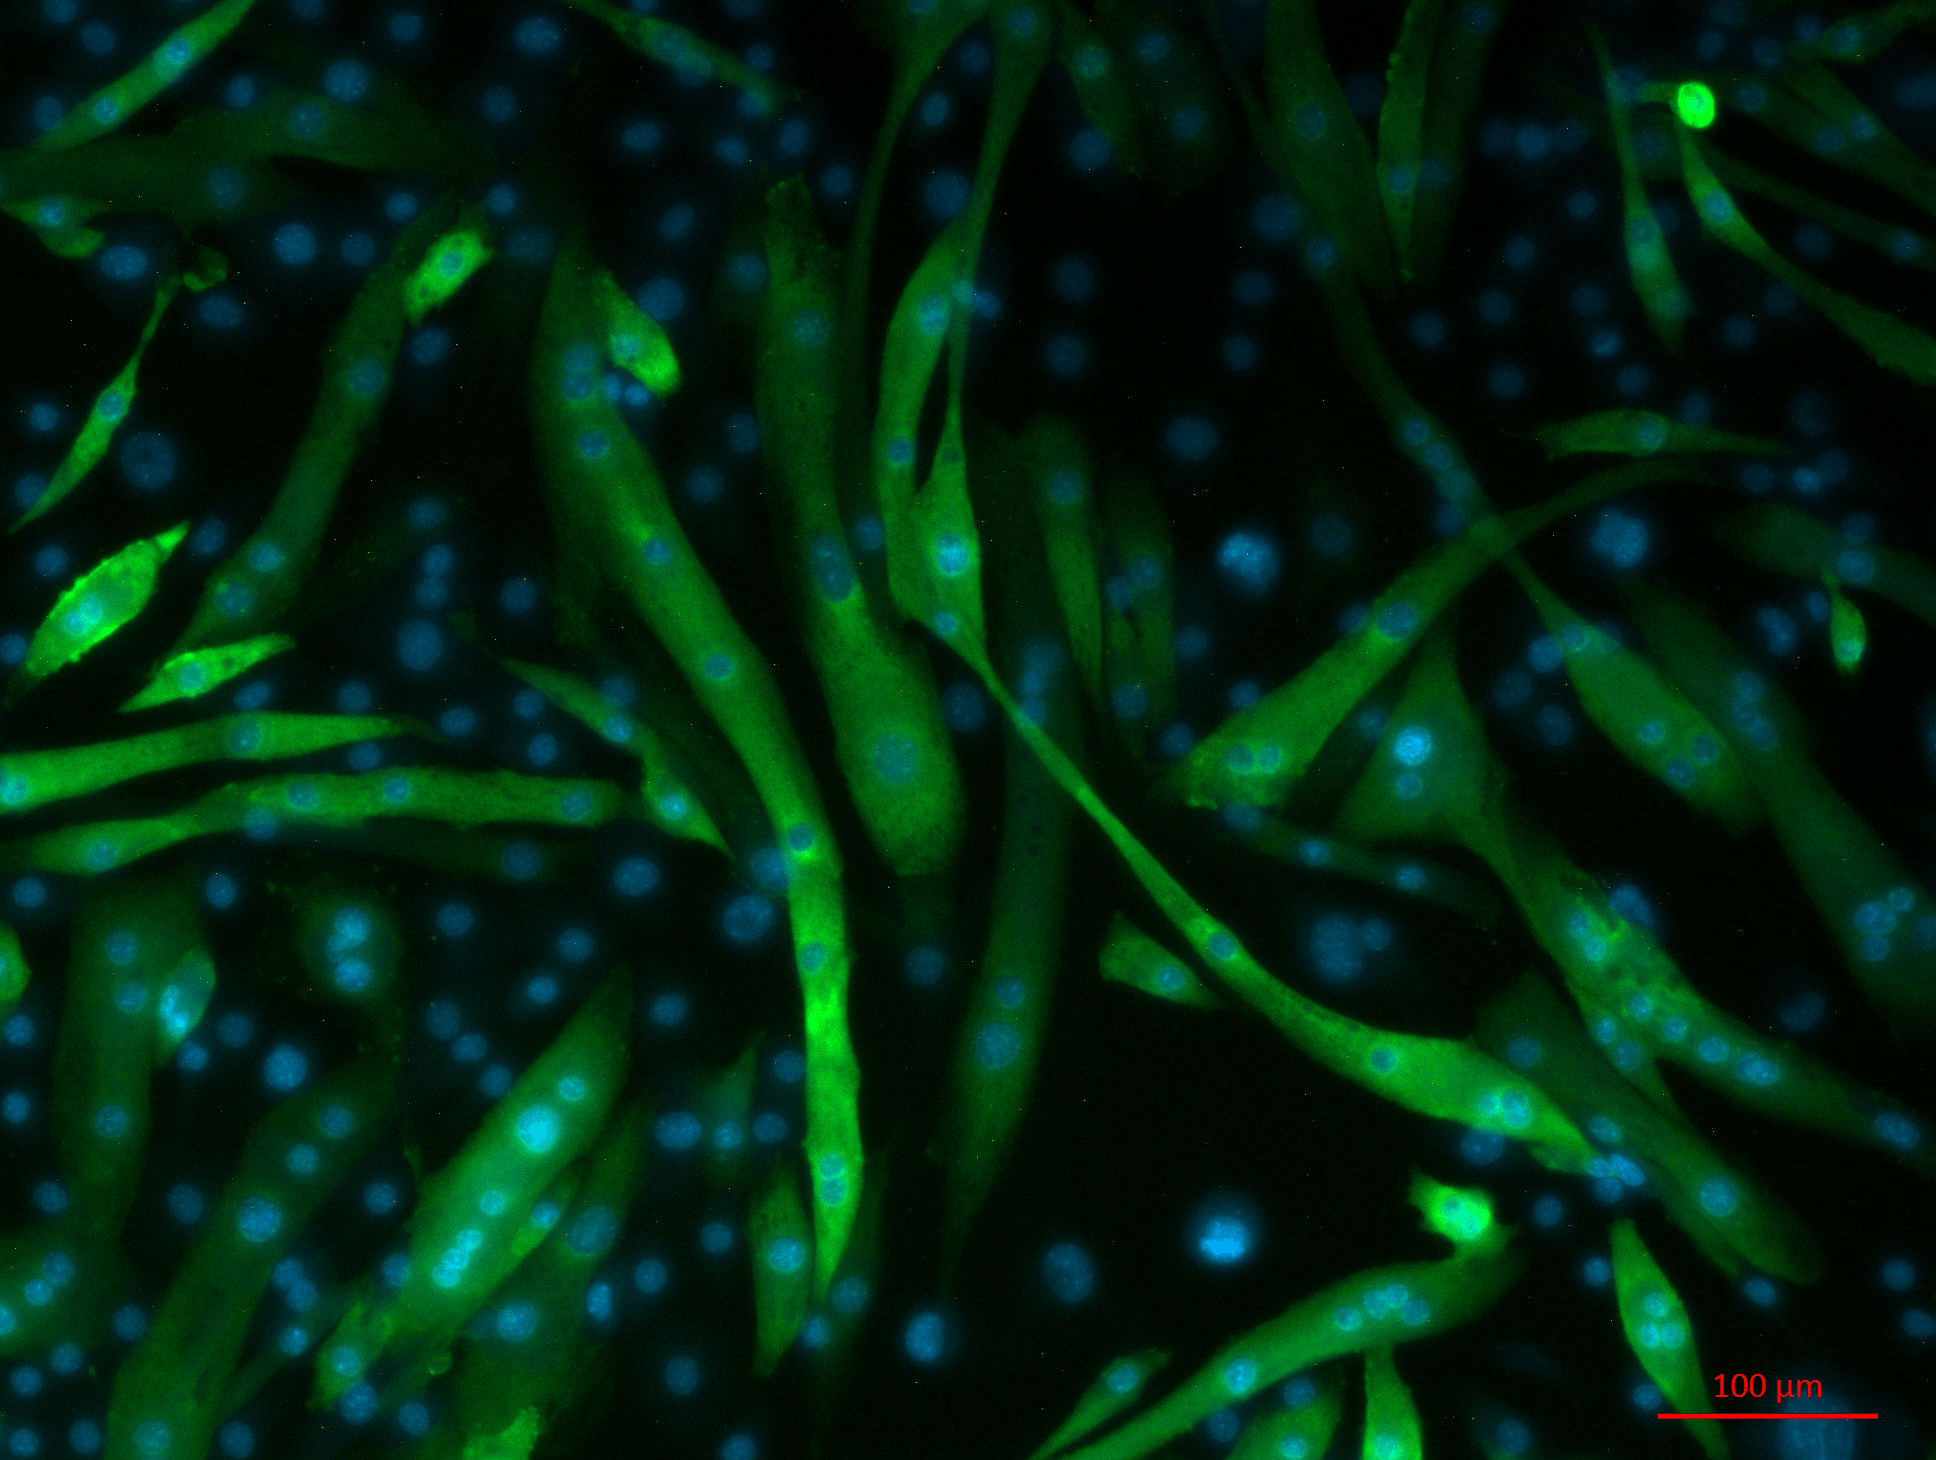
\includegraphics[width=\textwidth]{images/BDC_4_J_2_10X_c1-2.png}
	\end{subfigure}
	\hfill
	\begin{subfigure}{0.4\textwidth}
		\raggedright\textbf{B.}
		\vspace{0.15cm}
		
		\centering
		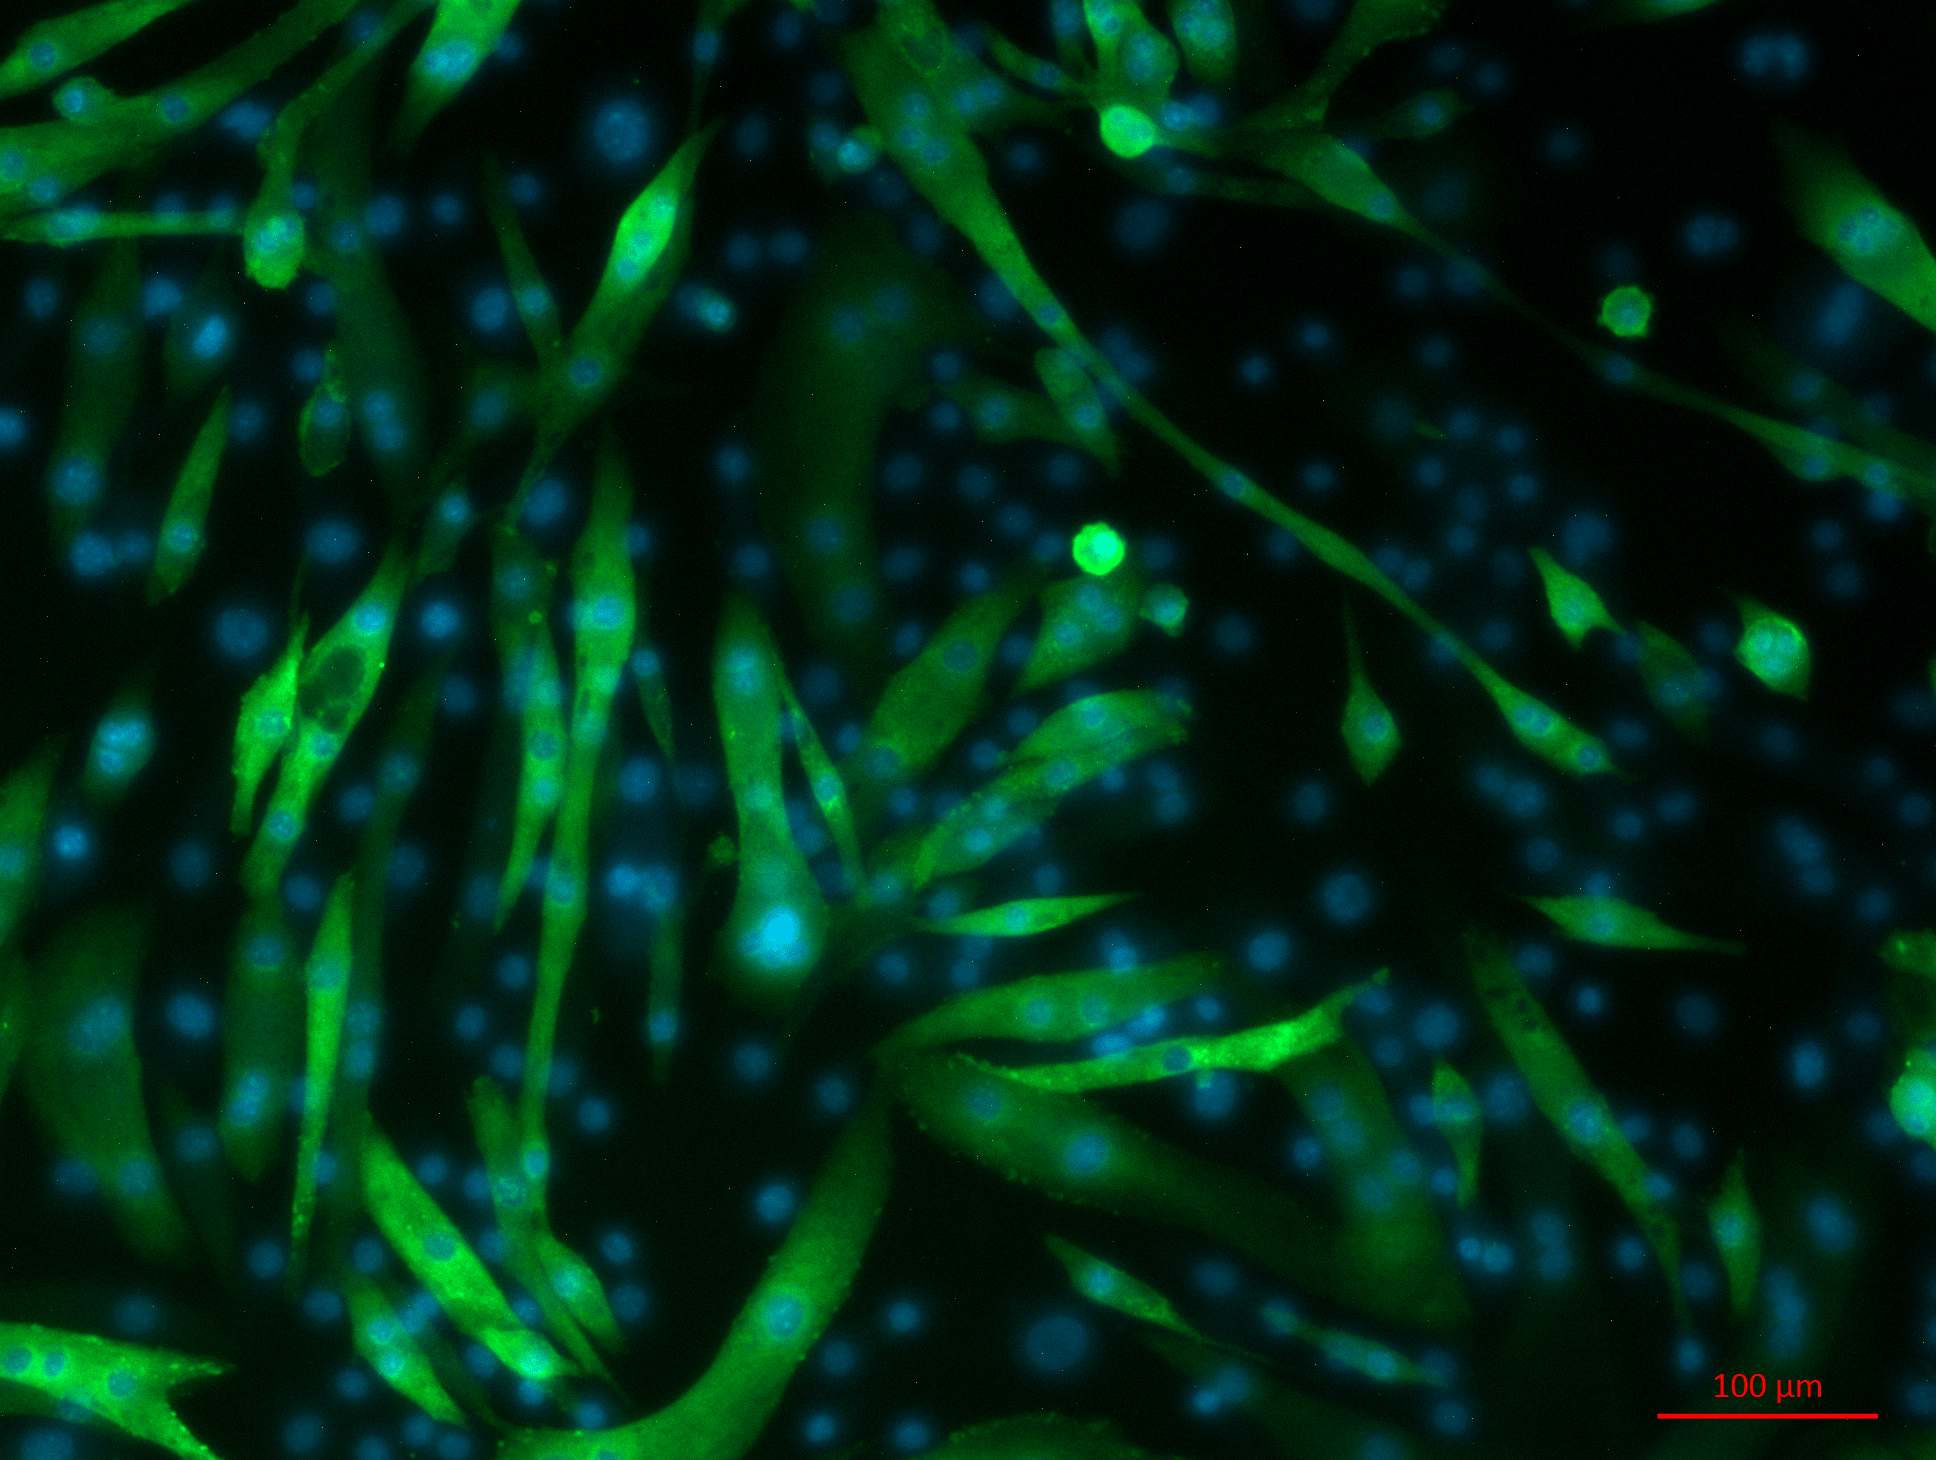
\includegraphics[width=\textwidth]{images/HDT6_J_6_10X_c1-2.png}
	\end{subfigure}
	
	\vspace{0.1cm}
	
	\begin{subfigure}{0.46\textwidth}
		\raggedright\textbf{C.}
		
		\centering
		\raisebox{0.2cm}{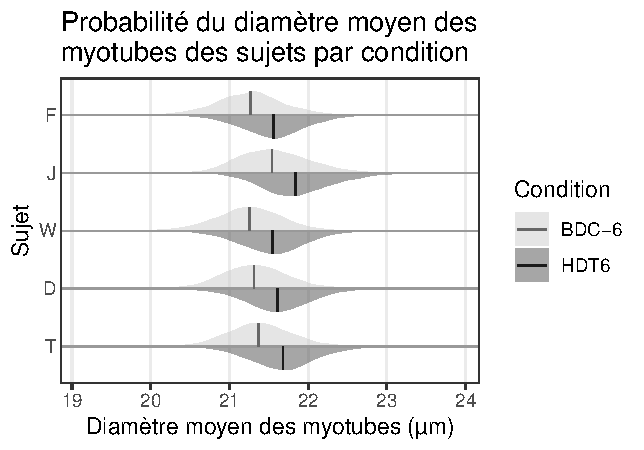
\includegraphics[width=\textwidth]{images/sujet.pdf}}
		
		\vspace{-0.5cm}
	\end{subfigure}
	\hfill
	\begin{subfigure}{0.38\textwidth}
		\vspace{0.4cm}
		\raggedright\textbf{D.}
		
		\centering
		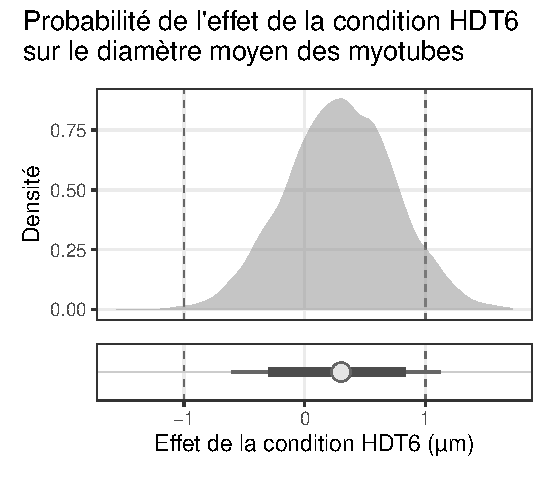
\includegraphics[width=\textwidth]{images/effet.pdf}
		
		\vspace{-0.5cm}
	\end{subfigure}
	
	\vspace{0.5cm}
	
	\caption[Résultats de l'analyse du diamètre des myotubes.]{\textbf{A.} Cliché représentatif en condition BDC-6 (6 jours avant le début du protocole d'alitement à -6°). \textbf{B.} Cliché représentatif en condition HDT6 (au bout de 6 jours de protocole d'alitement à -6°). \textbf{C.} Les traits verticaux correspondent au diamètre moyen des myotubes des sujets. A noter que le modèle statistique a été spécifié pour évaluer un effet fixe de la condition en tenant compte d'un effet aléatoire du sujet (voir section \ref{subsec:stat}). Ainsi, en condition HDT6 le diamètre moyen des myotubes correspond à la médiane de $\mu_{\alpha} + \beta$ pour chaque sujet. \textbf{D.} Les lignes verticales en pointillés indiquent les bornes de la ROPE (région d'équivalence pratique), fixées à |1| $\mu$m. Le point représente l'estimation de l'effet de la condition HDT6 sur le diamètre des myotubes par rapport à la condition BDC-6 (médiane de $\beta$). Les traits horizontaux fins et épais correspondent aux intervalles de crédibilité à 80\% et 95\%.}
	\label{fig:panel_myotubes}
\end{figure}

La probabilité du diamètre moyen des myotubes par condition pour chaque sujet est présentée dans la figure~\ref{fig:panel_myotubes}. La variabilité inter-sujet apparaît limitée : le paramètre $\sigma_{\alpha}$ est estimé à 1,01 (IC$_{95\%}$ = [1,00 ; 1,06]), indiquant une variation d'environ 1\% des diamètres moyens entre les sujets.

Dans la population, le diamètre moyen des myotubes en condition BDC-6 est estimé à 21,34 $\mu$m (médiane de $\mu_{\alpha}$), avec un intervalle de crédibilité à 95\% étroit (IC$_{95\%}$ = [20,59 ; 22,17]), traduisant une faible incertitude autour de cette estimation. En condition HDT6, le diamètre moyen des myotubes est estimé à 21,65 $\mu$m (médiane de $\mu_{\alpha} + \beta$), avec un IC$_{95\%}$ = [20,88 ; 22,48]. Ces résultats indiquent des valeurs très proches entre les deux conditions expérimentales.

\medskip La probabilité de l'effet de la condition HDT6 sur le diamètre des myotubes est présentée dans la figure~\ref{fig:panel_myotubes}. L'estimation de $\beta$ est de 0,30 $\mu$m (IC$_{95\%}$ = [-0,61 ; 1,13]), ce qui suggère une absence d'effet de la condition HDT6 sur le diamètre des myotubes par rapport à la condition BDC-6. Afin d'évaluer le sens biologique de cette estimation, une ROPE (région d'équivalence pratique) a été définie à |1| $\mu$m, correspondant à une variation considérée comme cliniquement négligeable. La probabilité que l'effet soit compris dans cet intervalle est de 94,0\% ($P(|\beta|<1$) = 0,940), indiquant une forte probabilité d'absence d'effet de la condition HDT6 sur le diamètre moyen des myotubes. En outre, la probabilité d'un effet correspondant à une atrophie ($P(\beta)<-1$) est très faible (0,3\%).

\section{Expression des protéines d'intérêt}

La probabilité \textit{a posteriori} de l'effet de la condition HDT6 sur l'expression de chaque protéine d'intérêt est présentée dans la figure~\ref{fig:densite_et_photo}. À l'exception des chaînes lourdes de myosine, l'estimation de l'effet de la condition HDT6 par rapport à la condition BDC-6 suggère une absence d'effet sur l'expression de l'ensemble des protéines d'intérêt. En effet, la majorité des distributions apparaissent largement comprises dans la ROPE, dont les bornes ont été fixées à 1 $\pm$ 0,2 (ratio HDT6/BDC-6). Il est recommandé que l'amplitude du changement observé entre deux conditions soit au moins deux fois supérieure au coefficient de variation des réplicats techniques \parencite{BibEntry2026Apr}. Toutefois, en l'absence d'un nombre suffisant de réplicats permettant une estimation fiable de ce coefficient, une valeur standard a été considérée.

\begin{figure}[h!]
	\centering
	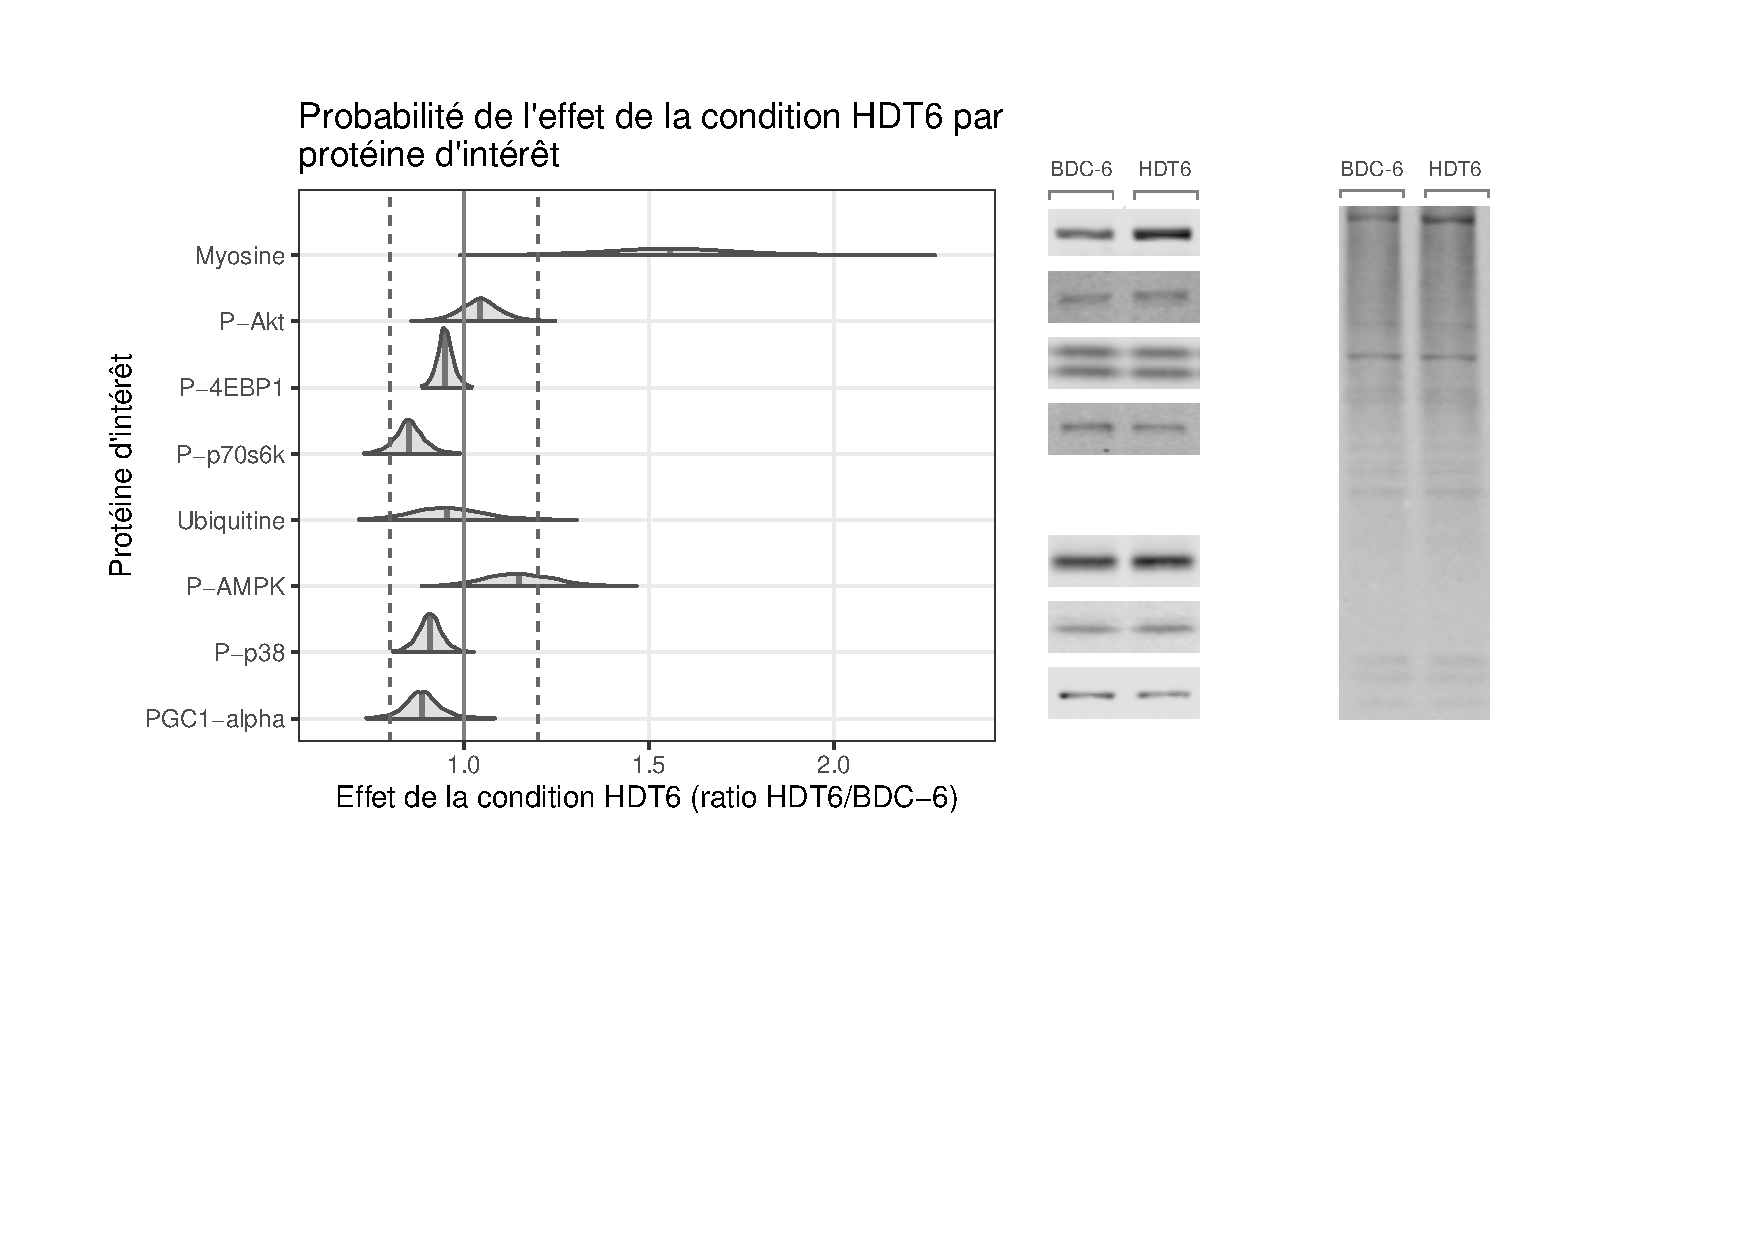
\includegraphics[scale=0.59]{images/résultats_WB.pdf}
	\caption[Résultats de l'analyse de l'expression des protéines d'intérêt.]{BDC-6 correspond au sixième jour précédant le début du protocole d'alitement à \mbox{-6°}, et HDT6 correspond au sixième jour de ce protocole. Les lignes verticales en pointillés indiquent les bornes de la ROPE (région d'équivalence pratique), fixées à 1 $\pm$ 0,2 (ratio HDT6/BDC-6). Le trait vertical gris foncé représente l'estimation de l'effet de la condition HDT6 sur l'expression de chaque protéine d'intérêt par rapport à la condition BDC-6 (médiane de $\beta$). Les images illustrent de manière représentative les résultats des Western Blot. Le profil à droite illustre l'expression des protéines ubiquitinées. Les résultats pour chaque patient et chaque condition sont disponibles en \hyperref[annexeJ]{annexe J}.}
	\label{fig:densite_et_photo}
\end{figure}

Pour les chaînes lourdes de myosine, l'estimation du paramètre $\beta$ est de 1,56 (ratio HDT6/BDC-6), avec un IC$_{95\%}$ = [1,16 ; 1,98]. Cet intervalle de crédibilité traduit une très grande incertitude autour de cette estimation. Néanmoins, la probabilité \textit{a posteriori} d'un effet correspondant à une augmentation au-delà du seuil de 20\% est élevée ($P(\beta > 1,2) = 0,963$), suggérant une augmentation probable de l'expression des chaînes lourdes de myosine en condition HDT6. Le résumé des distributions postérieures de l'estimation de l'effet de la condition HDT6 sur l'expression de chaque protéine d'intérêt est présenté dans le tableau~\ref{table:WB}. Pour l'ensemble des marqueurs, hormis les chaînes lourdes de myosine, la probabilité que l'effet se situe dans la ROPE ($P(0,8 < \beta < 1,2)$) est systématiquement élevée, supérieure ou égale à 0,70, confirmant une absence d'effet clinique de la condition HDT6.

\begin{table}[ht]
	\centering
	\renewcommand{\arraystretch}{1.7}
	\begin{tabularx}{\textwidth}{
			>{\raggedright\arraybackslash}p{2cm}
			>{\centering\arraybackslash}p{1.2cm}
			>{\centering\arraybackslash}p{2.2cm}
			>{\centering\arraybackslash}X
			>{\centering\arraybackslash}p{3cm}
			>{\centering\arraybackslash}p{2cm}
			>{\centering\arraybackslash}p{2.3cm}
		}
		\hline
		Protéine &
		Médiane de $\beta$ &
		IC$_{95\%}$ &
		$P_{\text{dir}}$ &
		\textbf{$P(0,8<\beta<1,2)$} &
		\textbf{$P(\beta<0,8)$} &
		\textbf{$P(\beta>1,2)$} \\
		\hline
		\textbf{Myosine} & 1,56 & [1,16 ; 1,98] & 0,997(+) & 0,037 & 0,000 & 0,963 \\
		\textbf{P-Akt} & 1,04 & [0,90 ; 1,18] & 0,799(+) & 0,980 & 0,003 & 0,017 \\
		\textbf{P-4EBP1} & 0,95 & [0,91 ; 1,00] & 0,979(-) & 1,000 & 0,000 & 0,000 \\
		\textbf{P-p70S6K} & 0,85 & [0,76 ; 0,95] & 0,993(-) & 0,908 & 0,092 & 0,000 \\
		\textbf{Ubiquitine} & 0,95 & [0,77 ; 1,17] & 0,703(-) & 0,932 & 0,051 & 0,017 \\
		\textbf{P-AMPK} & 1,15 & [0,96 ; 1,36] & 0,943(+) & 0,706 & 0,001 & 0,293 \\
		\textbf{P-p38} & 0,91 & [0,84 ; 0,98] & 0,990(-) & 0,998 & 0,002 & 0,000 \\
		\textbf{PGC1-$\bm{\alpha}$} & 0,89 & [0,78 ; 1,01] & 0,972(-) & 0,951 & 0,048 & 0,001 \\
		\hline
	\end{tabularx}
	\caption[Résumé des distributions postérieures de l'estimation de l'effet de la condition HDT6 sur l'expression des protéines d'intérêt (ratio HDT6/BDC-6).]{Résumé des \textit{posteriors} de l'estimation de l'effet de la condition HDT6 sur l'expression de chaque protéine d'intérêt (ratio HDT6/BDC-6). La médiane de $\beta$ représente l'estimation de l'effet de la condition HDT6 sur l'expression des protéines par rapport à la condition BDC-6. BDC-6 correspond au sixième jour précédant le début du protocole d'alitement à -6°, et HDT6 correspond au sixième jour de ce protocole. IC$_{95\%}$ correspond à l'intervalle de crédibilité à 95\%, indiquant une probabilité de 95\% que le paramètre se situe dans cet intervalle, conditionnellement aux données et au modèle. $P_{\text{dir}}$ correspond à la probabilité \textit{a posteriori} que l'effet soit dans une direction donnée. $P(0,8<\beta<1,2)$ correspond à la probabilité \textit{a posteriori} d'un effet négligeable, tandis que $P(\beta<0,8)$ et $P(\beta>1,2)$ reflètent respectivement la probabilité d'un effet cliniquement significatif négatif ou positif.}
	\label{table:WB}
\end{table}

Concernant les voies de synthèse protéique, les probabilités \textit{a posteriori} d'une diminution cliniquement significative de l'expression p-Akt, p-4EBP1 et p-p70S6K sont très faibles. Elles sont respectivement égales à 0,3\%, 0,0\% et 9,2\%. De plus, la probabilité \textit{a posteriori} d'une augmentation cliniquement significative de l'expression des protéines ubiquitinées est faible ($P(\beta > 1,2) = 0,017$), tout comme celle de p-p38 ($P(\beta > 1,2) = 0,000$). Seul p-AMPK présente une probabilité plus élevée ($P(\beta > 1,2) = 0,293$), associée à une probabilité de direction importante ($P_{\text{dir}} = 0,943$), mais l'intervalle de crédibilité reste large (IC$_{95\%}$ = [0,96 ; 1,36]), limitant l'interprétation de la taille de cet effet. Enfin, en ce qui concerne la biogenèse mitochondriale, la probabilité \textit{a posteriori} d'une diminution cliniquement significative de l'expression de PGC1-$\alpha$ est limitée ($P(\beta < 0,8) = 0,048$).

\medskip Ainsi, ces résultats indiquent qu'à l'exception d'une augmentation probable de l'expression des chaînes lourdes de myosine, la condition HDT6 ne semble pas avoir d'effet sur les principales voies impliquées dans la synthèse, la dégradation protéique ou la biogenèse mitochondriale.

% Discussion
\chapter{Discussion}

L'objectif de ce mémoire était de déterminer si l'environnement systémique avait un effet sur le phénotype contractile et métabolique du muscle squelettique d'individus exposés à la microgravité simulée. Pour cela, des myotubes C2C12 ont été exposés pendant 48 heures à du plasma prélevé 6 jours avant (BDC-6) et 6 jours après un protocole d'alitement à -6° (HDT6). Nous avons fait l'hypothèse que le plasma prélevé après 6 jours de protocole induirait un phénotype d'atrophie, caractérisé notamment par une réduction du diamètre des myotubes et une diminution de la quantité totale de myosine.

Le diamètre moyen des myotubes est resté inchangé entre les conditions BDC-6 et HDT6, sans signe d'atrophie macroscopique. En dépit de ce résultat, une augmentation de l'expression des chaînes lourdes de myosine a été observée en condition HDT6, bien que cet effet demeure incertain. De plus, aucun marqueur d'inhibition de la synthèse protéique (p-Akt, p-4EBP1, p-p70S6K), d'activation de la protéolyse (protéines ubiquitinées), d'augmentation du stress cellulaire (p-AMPK, p-p38) ou de diminution de la biogenèse mitochondriale (PGC1-$\alpha$) n'a été mis en évidence. Ainsi, le plasma post-alitement n'a pas induit les voies de signalisation classiquement associées à l'atrophie musculaire.

\section{Effet de l'environnement systémique sur le phénotype musculaire}

\subsection{Absence d'atrophie induite par le plasma et rôle de l'état inflammatoire}

L'absence d'effet de la condition HDT6 sur le diamètre des myotubes et sur l'expression de l'ensemble des protéines d'intérêt, à l'exception des chaînes lourdes de myosine, par rapport à la condition BDC-6, indique que l'environnement systémique isolé, dans notre modèle, ne suffit pas à induire un phénotype d'atrophie musculaire \textit{in vitro}, invalidant nos hypothèses.

Pourtant, si les adaptations musculaires observées lors de l'exposition à la microgravité sont largement attribuées à l'absence de contraintes mécaniques, elles s'accompagnent également d'adaptations systémiques susceptibles de moduler les voies de synthèse et de dégradation protéique, et donc d'influencer les adaptations du muscle squelettique \parencite{lee_factors_2022}. A notre connaissance, aucune étude ne s'est intéressée au traitement de cellules musculaires avec du plasma ou du sérum de patients ayant été exposés à une microgravité réelle ou simulée. Le design expérimental le plus proche du nôtre est celui de \textcite{Kalampouka2018Feb}, qui ont montré une diminution du diamètre de myotubes C2C12 après 24 et 48 heures de traitement avec du plasma de sujets âgés (>57 ans), comparativement à celui de sujets jeunes (18-35 ans). Ces résultats peuvent s'expliquer par les modifications de l'environnement systémique associées au vieillissement, qui incluent une diminution de facteurs anaboliques \parencite{Sellami2017Aug,Ratkevicius2011Jun}, et une élévation de cytokines pro-inflammatoires \parencite{Alvarez-Rodriguez2012}. Or, les missions spatiales de longue durée induisent une réponse inflammatoire comparable associée à un phénotype immunitaire qualifié d'« inflammaging » \parencite{navasiolava_vascular_2020,strollo_aging-like_2021}. C'est pourquoi anticiper un phénotype d'atrophie paraissait cohérent. Toutefois, les périodes de courte inactivité n'entraîneraient pas nécessairement de modifications des marqueurs systémiques \parencite{navasiolava_vascular_2020}. Par conséquent, l'implication d'un état pro-inflammatoire dans les adaptations musculaires précoces à la microgravité, tant réelle que simulée, demeure dans la littérature incertaine. Un effet catabolique du plasma sur des myotubes a principalement été rapporté dans des contextes pathologiques marqués par une inflammation systémique. Par exemple, \textcite{vanHees2011} ont montré une diminution d'environ 25\% du contenu en myosine de myotubes exposés au plasma de patients atteints de septicémie, associée à une augmentation de l'expression de MuRF1 et MAFbx, ainsi qu'à une accumulation des protéines ubiquitinées. Dans ce contexte, l'absence d'effet observée dans notre protocole pourrait s'expliquer par un état inflammatoire peu altéré après 6 jours d'alitement à -6° chez des sujets sains.

Dans le cadre du protocole d'AGBRESA, seuls des marqueurs indirects de l'inflammation ont été dosés, notamment la CRP (protéine C-réactive), la ferritine et l'haptoglobine, des protéines de phase aiguë. En particulier, la CRP, synthétisée par les hépatocytes sous le contrôle transcriptionnel de l'IL-6, et dans une moindre mesure de l'IL-1$\beta$ et du TNF-$\alpha$, constitue un marqueur reconnu de l'inflammation \parencite{Rizo-Tellez2023Jul}. Dans nos données, les concentrations en CRP restent faibles dans les deux conditions (BDC-6 : 0,87 $\pm$ 0,99 mg.L$^{-1}$ ; HDT6 : 0,43 $\pm$ 0,37 mg.L$^{-1}$), largement en dessous du seuil de 3 mg.L$^{-1}$ utilisé pour définir une inflammation systémique \parencite{Wieczorek2021Sep}. De même, la ferritine ne présente pas de variation majeure entre BDC-6 (58, 2 $\pm$ 48,9 $\mu$g.L$^{-1}$) et HDT6 (62,0 $\pm$ 51,7 $\mu$g.L$^{-1}$), tout comme l'haptoglobine (BDC-6 : 1,04 $\pm$ 0,58 g.L$^{-1}$ ; HDT6 : 1,05 $\pm$ 0,44 g.L$^{-1}$). L'ensemble de ces paramètres, détaillés pour chacun des participants en \hyperref[annexeH]{annexe H}, suggère donc un état inflammatoire peu modifié après 6 jours d'alitement à -6°. Il aurait néanmoins été intéressant de disposer de mesures de marqueurs directs de l'inflammation, en particulier de l'IL-6, afin de confirmer cette interprétation, cette cytokine étant reconnue pour sa sensibilité aux variations, même modestes, de l'état inflammatoire. Un faible niveau de réponse inflammatoire paraît cohérent avec la littérature. En effet, bien que des modifications des concentrations plasmatiques des cytokines aient déjà été rapportées dans des protocoles d'alitement à -6°, la présence d'une réponse inflammatoire de bas grade dans ce contexte précis reste peu établie. \textcite{Feuerecker2013Jul} et \textcite{Bonnefoy2022Feb} ne montrent ainsi aucune variation significative de la concentration en cytokines pro-inflammatoires au bout de 3 et 5 jours d'alitement à -6° et jusqu'à 60 jours. A l'inverse, \textcite{Schmitt2000} rapportent des résultats plus contrastés en décrivant une absence de modification de la concentration de TNF-$\alpha$ sur 34 jours d'alitement à -6°, alors que les niveaux d'IL-1$\beta$ sont augmentés. Par ailleurs, lors d'un protocole plus prolongé, une augmentation de l'IL-6 a été décrite, mais celle-ci a été attribuée au stress psychologique plutôt qu'à une réponse inflammatoire avérée, les autres cytokines pro-inflammatoires restant inchangées \parencite{Chouker2001May}. L'état inflammatoire au cours d'un protocole d'alitement à -6° apparaît donc soit absent, soit modéré, et reste à caractériser plus précisément. Surtout, il demeure sans commune mesure avec les contextes pathologiques associés à une inflammation systémique. Les concentrations d'IL-6 chez des sujets sains sont en effet estimées autour de 5,2 pg.mL$^{-1}$ \parencite{Said2021Jun}, tandis qu'elles atteignent des niveaux bien plus élevés chez des patients en état critique ($\approx$ 100,9 pg.mL$^{-1}$) \parencite{Picod2022May}. Dans ce contexte, même si une inflammation de bas grade ne peut être totalement exclue chez nos participants, celle-ci reste vraisemblablement limitée, ce qui contribue certainement à expliquer l'absence d'effet de la condition HDT6 sur le diamètre des myotubes et sur l'expression des différentes protéines d'intérêt dans notre protocole.

Nos résultats n'excluent toutefois pas l'existence d'un effet d'interaction. Effectivement, les adaptations systémiques observées en microgravité réelle ou simulée pourraient amplifier les adaptations musculaires causées par l'absence de contraintes mécaniques, produisant un effet combiné supérieur à la somme des effets de ces facteurs isolés. Par exemple, la voie mTOR peut être activée indépendamment par des stimuli mécaniques ou par des facteurs de croissance \parencite{Hornberger2004Jun,Jacobs2013Oct}. Ainsi, bien qu'aucun effet indépendant de l'environnement systémique n'ait été mis en évidence sur le diamètre des myotubes ou sur l'expression des protéines d'intérêt, un effet synergique reste possible. Par ailleurs, un effet de médiation ne peut être exclu. L'utilisation \textit{ex vivo} de plasma nous a permis d'exposer les myotubes à un environnement systémique spécifique tout en supprimant l'impact direct des stimuli mécaniques. Nos résultats ne permettent pas de rendre compte des régulations systémiques qui auraient été elles-mêmes induites par les modulations de la synthèse et de la dégradation protéique du fait de l'absence de contraintes mécaniques au-delà des 6 jours de protocole. A ce titre, la myostatine, régulateur négatif de la masse musculaire, augmente après 25 jours d'alitement à -6° \parencite{Zachwieja1999Oct}, mais il est possible qu'en condition HDT6 son augmentation soit absente ou encore limitée. Dans cette perspective, l'environnement systémique pourrait intervenir comme médiateur des adaptations musculaires observées.

\subsection{Interprétation de l'expression des chaînes lourdes de myosine}

Nos résultats montrent une augmentation probable de l'expression des chaînes lourdes de myosine. L'estimation du paramètre $\beta$ est de 1,56 (ratio HDT6/BDC-6), ce qui paraît peu cohérent avec l'absence d'effet observée par ailleurs sur le diamètre des myotubes et sur l'expression des autres protéines étudiées. L'intervalle de crédibilité associé à cette estimation demeure large (IC$_{95\%}$ = [1,16 ; 1,98]), ce qui invite à une interprétation prudente. L'ampleur de cette augmentation pourrait être influencée par le choix arbitraire des bornes de la ROPE, fixées à 1 $\pm$ 0,2 (ratio HDT6/BDC-6). Dans le cas présent, nous ne disposions que de deux réplicats biologiques sans réplicats techniques, ne permettant pas d'estimer le coefficient de variation associé. Une valeur élevée de ce coefficient pourrait remettre en question l'analyse quantitative proposée \parencite{BibEntry2026Apr}. Cependant, l'examen qualitatif des images (disponibles en \hyperref[annexeJ]{annexe J}), suggère bien une augmentation de l'expression des chaînes lourdes de myosine entre les deux conditions, même si cet effet apparaît moins marqué dans l'expérience indépendante n°2. 

Une augmentation de l'expression des chaînes lourdes de myosine n'implique toutefois pas nécessairement une hypertrophie : le plasma peut favoriser la différenciation des myotubes et donc l'expression des chaînes lourdes de myosine. Pour une même quantité de protéines par puits, la proportion des chaînes lourdes de myosine pourrait donc augmenter, mais cette interprétation reste à nuancer car les deux conditions ont été soumises à des modalités expérimentales identiques. Afin de s'assurer que l'effet observé reflète une modification biologique effective, de nouvelles expérimentations seraient nécessaires.

\section{Transposabilité à d'autres modèles de microgravité}

Aucun effet indépendant de l'environnement systémique n'a été mis en évidence, à l'exception de l'expression des chaînes lourdes de myosine. Ce résultat pourrait en partie dépendre des conditions expérimentales, notamment de la concentration de plasma utilisée et de la durée de traitement des myotubes. Néanmoins, bien que les paramètres permettant de reproduire au mieux un environnement systémique physiologique \textit{in vitro} restent à préciser, il paraît peu probable que l'absence d'effet observé soit imputable au design expérimental car des phénotypes d'atrophie ont déjà été rapportés dans des conditions expérimentales similaires \parencite{Allen2022Dec}. La question d'un effet de l'environnement systémique sur le phénotype contractile et métabolique du muscle squelettique de participants exposés à un autre protocole de microgravité simulée, l'immersion sèche, reste cependant ouverte. En effet, la présence d'un état pro-inflammatoire dans ce contexte demeure débattue. Une augmentation de l'IL-6 a par exemple été rapportée après quatre jours d'immersion sèche \parencite{Twomey2021Nov}, tandis que d'autres auteurs n'ont pas observé de modification des cytokines pro-inflammatoires après trois, cinq et sept jours de protocole \parencite{Moser2026Feb,Berendeeva2011Dec}, ou ont rapporté des résultats contrastés \parencite{fovet_early_2021}. De même, la question se pose toujours pour la microgravité réelle, d'autant que les vols spatiaux de longue durée sont, eux, associés à un état inflammatoire chronique de bas grade avéré \parencite{Crucian2014Oct,Buchheim2019Feb,Krieger2021Aug}. Enfin, notre protocole portait sur des sujets sains. Dans des contextes physiopathologiques caractérisés par une inflammation plus sévère, celle-ci est reconnue comme contribuant fortement à l'atrophie \parencite{Puthucheary2013Oct,Fazzini2023Dec,mehdi_endocrine_2025,Damanti2024Oct}.

\section{Forces, limites et perspectives}

\subsection{Forces, limites et perspectives méthodologiques}

Ce mémoire constitue, à notre connaissance, la première utilisation d'un modèle de milieu conditionné avec du plasma issu d'un protocole de microgravité simulée. Par ailleurs, le recours à des échantillons individuels, plutôt que poolés, permet de préserver la variabilité biologique interindividuelle et d'approcher davantage les conditions \textit{in vivo}. Néanmoins, notre modèle ne permet pas d'analyser un éventuel remodelage typologique des fibres musculaires. En effet, en l'absence de stimulation spécifique, notamment de flux calciques, les myotubes différenciés \textit{in vitro} présentent majoritairement un phénotype rapide de type II \parencite{Lu2023Sep}. De plus, l'absence de mesure de marqueurs inflammatoires directs dans les plasmas limite l'interprétation de nos résultats.

En outre, ce modèle de milieu conditionné constitue un design expérimental permettant d'isoler l'effet de l'environnement systémique de celui de l'absence de contrainte mécanique. Il contribue également à pallier en partie le manque de pertinence écologique généralement attribué aux approches \textit{in vitro}. Toutefois, la culture cellulaire en deux dimensions présente certaines limites : elle ne permet pas le maintien de l'organisation structurale des cellules dans le temps et ne reproduit pas fidèlement les interactions cellule-cellule et cellule-matrice extracellulaire \parencite{Perez-Diaz2025Jun}. Dans ce contexte, les modèles tridimensionnels, tels que les systèmes \textit{organ-on-a-chip}, les tissus bio-ingénierés ou les agrégats cellulaires, suscitent un intérêt croissant en raison de leur capacité à mieux reproduire la complexité du muscle squelettique \textit{in vitro}. Leur utilisation pourrait constituer une perspective intéressante tant pour caractériser l'effet de l'environnement systémique que celui de l'absence de contraintes mécaniques sur le muscle squelettique en microgravité réelle ou simulée. De plus, l'utilisation de myotubes humains, tels que la lignée LHCN-M2, associée à du plasma ou du sérum d'origine humaine, pourrait améliorer la transposabilité des observations dans différents contextes physiopathologiques.

Par ailleurs, le recours aux modèles \textit{in vitro} ne relève pas uniquement de considérations techniques, mais dépend aussi d'orientations sociopolitiques et éthiques. Il permet de limiter l'expérimentation animale, en accord avec le principe des 3R (\textit{Replacement, Reduction, Refinement}) introduit par \textcite{Russell1959} et largement adopté par la communauté scientifique, les autorités et les industries \parencite{Rosolowski2025Nov}. Néanmoins, il est important de noter que l'utilisation de produits dérivés d'origine animale soulève des questions éthiques persistantes \parencite{Grimm2023Jun}.

\subsection{Forces et limites de l'inférence bayésienne}

\medskip Ce mémoire représente aussi, à notre connaissance, une première application de l'inférence bayésienne dans l'analyse de données de diamètre de myotubes et de Western Blot. \textcite{Crook2022Apr} avaient déjà souligné que les statistiques bayésiennes présentaient un potentiel considérable pour l'analyse de données de protéomique, bien qu'elles soient peu adoptées dans la communauté en biologie. Dans notre cas, la structure des données se prêtait particulièrement bien à l'utilisation de modèles hiérarchiques et nous a permis de quantifier les différences entre les deux conditions en termes de probabilité. Cette approche nous a permis d'obtenir une estimation de la différence du diamètre des myotubes avec une incertitude faible, ainsi que de calculer la probabilité de variations d'expression des protéines analysées par Western Blot. Cependant, l'absence de données suffisantes ne nous a pas permis de choisir une ROPE (région d'équivalence pratique) précise répondant aux recommandations faites pour l'analyse quantitative de résultats de Western Blot \parencite{BibEntry2026Apr}. Dans le cas où on disposerait d'un plus grand nombre d'observations par protéines, la réalisation d'un modèle bayésien multivarié parait intéressante. Un tel modèle permettrait la prise en compte de corrélations entre les différentes protéines d'intérêt et considérerait que l'information soit partagée entre ces paramètres. 

Enfin, \textcite{Gosselin2022} soulignent que, dans un grand nombre d'études réalisant des analyses quantitatives de résultats de Western Blot, les procédures statistiques sont peu ou pas décrites, et reposent fréquemment sur de très faibles tailles d'échantillon. Ces conditions diminuent fortement la puissance statistique des analyses et peuvent par exemple empêcher la détection de différences significatives aux seuils usuels. \textcite{Gosselin2022} conclut donc qu'une part importante de la littérature dans ce domaine pourrait reposer sur des résultats peu fiables, contribuant à la crise de la reproductibilité. Dans ce contexte, la mise en place de recommandations méthodologiques claires en matière de quantification et d'analyse statistique apparaît nécessaire. L'inférence bayésienne constitue à cet égard une piste intéressante : bien qu'elle nécessite un effort de formation, elle favorise la transparence des analyses et concilie le traitement objectif de données empiriques avec les connaissances issues \textit{a priori} de la littérature et de l'expertise, dans un cadre plus informatif.

\subsection{Population étudiée et perspectives}

Nous avons inclus à la fois des participants masculins et féminins, ce qui constitue un atout dans la mesure où des travaux s'intéressant aux femmes restent sous-représentés dans ce domaine. Pour autant, la taille de notre échantillon étant limitée, le sexe des participants pourrait représenter une variable de confusion dans nos analyses. Des travaux futurs incluant un plus grand nombre de participants permettraient de constituer des groupes distincts selon le sexe.

Pour finir, nous nous sommes principalement intéressés au phénotype contractile du muscle squelettique. Des investigations supplémentaires portant plus en détail sur les adaptations métaboliques auraient été intéressantes. Par ailleurs, notre approche était ici musculo-centrée, mais si de futures applications visaient directement les vols spatiaux, l'ensemble des facteurs de stress associés, au-delà de la microgravité, devrait être considéré notamment l'hypercapnie, les radiations et le stress psychologique.

\section{Implications pratiques}

Nos résultats, à l'exception de ceux relatifs à l'expression des chaînes lourdes de myosine, indiquent que l'environnement systémique, indépendamment de l'absence de contraintes mécaniques, ne suffit pas à induire un phénotype d'atrophie. Cela renforce l'idée que l'absence de contraintes mécaniques est bien le déterminant principal de l'atrophie observée en microgravité. Par conséquent, les contre-mesures permettant une sollicitation mécanique du muscle, en particulier les exercices physiques, mais aussi potentiellement la gravité artificielle, apparaissent comme les approches les plus prometteuses pour limiter le déconditionnement musculaire des astronautes.

Sur le plan clinique, la diminution des contraintes mécaniques due à l'alitement mais aussi l'état inflammatoire du patient sont susceptibles de contribuer aux adaptations musculaires. Les exercices physiques représentent donc aussi une stratégie intéressante, mais des travaux supplémentaires sont nécessaires afin d'en préciser les modalités optimales, notamment quand débuter l'intervention, quelle intensité privilégier et quels traitements y associer.

% Conclusion
\chapter{Conclusion}

Ce mémoire visait à déterminer si l'environnement systémique avait un effet sur le phénotype contractile et métabolique du muscle squelettique d'individus exposés à la microgravité simulée. Le diamètre moyen des myotubes est resté inchangé entre les conditions BDC-6 et HDT6, sans signe d'atrophie macroscopique. Le plasma post-alitement n'a pas non plus induit les voies de signalisation classiquement associées à l'atrophie musculaire. Cependant, une augmentation de l'expression des chaînes lourdes de myosine a été observée en condition HDT6, bien que cet effet demeure incertain et demande à être confirmé.

Ces résultats paraissent cohérents avec la littérature, dans la mesure où la présence d'une réponse inflammatoire de bas grade au cours de protocoles d'alitement à -6° n'est pas clairement établie. En l'absence de mesures de marqueurs directs de l'inflammation, une inflammation de bas grade ne peut être totalement exclue chez nos participants, mais elle reste vraisemblablement limitée, ce qui contribue certainement à expliquer l'absence d'effet de la condition HDT6 sur le diamètre des myotubes et sur l'expression des différentes protéines d'intérêt. Surtout, cet éventuel état inflammatoire demeure sans commune mesure avec les contextes pathologiques associés à une inflammation systémique. La question d'un effet de l'environnement systémique chez des participants exposés à un protocole d'immersion sèche ou à une microgravité réelle reste néanmoins ouverte.

Nos résultats renforcent l'idée que l'absence de contraintes mécaniques constitue le déterminant principal de l'atrophie observée en microgravité. Ils soutiennent ainsi l'intérêt des exercices physiques dans la prévention du déconditionnement musculaire, tant chez les astronautes que chez les patients.

\newpage
% Bibliographie
\pagestyle{empty}

\begingroup
\small % Ajuste la taille de la police
\setstretch{1.0} % Ajuste l'interligne
\printbibliography
\endgroup

\clearpage

% Annexe
\appendix
\onehalfspacing
\normalsize

\chapter*{Annexes}
\thispagestyle{empty}

\subsection*{Annexe A. Recherche bibliographique systématique}\phantomsection \label{annexeA}

Une recherche bibliographique systématique utilisant la méthodologie PRISMA-S a été effectuée \parencite{Rethlefsen2021Jan,Page2021Mar}. 

La stratégie de recherche a été élaborée selon le cadre PICO défini dans le tableau~\ref{table:PICO}.

\begin{table}[ht]
	\centering
	\renewcommand{\arraystretch}{1.7}
	\begin{tabularx}{\textwidth}{
			>{\raggedright\arraybackslash}p{4cm}
			>{\raggedright\arraybackslash}X
		}
		\hline
		\textbf{Catégorie} & \textbf{Description} \\
		\hline
		Patient & Humains \newline Cellules musculaires (humaines ou animales) \\
		\hline
		Intervention & Exposition à la microgravité (réelle ou simulée) \newline Traitement in vitro/ex vivo avec sérum/plasma \\
		\hline
		Comparaison & / \\
		\hline
		Outcomes & Muscle : masse, volume, type de fibre, phénotype contractile et métabolique, plasticité \newline Environnement systémique : métabolisme, substrats, hormones, hémodynamique, inflammation \\
		\hline
	\end{tabularx}
	\caption{Cadre PICO défini pour la recherche bibliographique systématique.}
	\label{table:PICO}
\end{table}

Les bases de données PubMed et Web of Science ont été consultées le 07/09/2025. Trois équations de recherche ont été définies pour chaque base, ciblant les adaptations musculaires en microgravité (Eq.1.), les mécanismes cellulaires sous-jacents et les adaptations systémiques (Eq.2.), ainsi que les méthodes de culture \textit{in vitro} et \textit{ex vivo}. Ces trois équations ont été combinées à l'aide de l'opérateur booléen OR. Les équations finales sont présentées dans les figures~\ref{fig:recherche_pubmed} et~\ref{fig:recherche_wos}.

\medskip Les doublons ont été supprimés à l'aide de l'outil d'identification automatique de \href{https://www.rayyan.ai/}{Rayyan}, puis vérifiés manuellement. Les références restantes ont ensuite fait l'objet d'un \textit{screening} manuel.

Les articles retenus devaient répondre aux critères du cadre PICO défini précédemment. Seules les publications en anglais ou en français ont été considérées. Les documents inclus comprenaient les articles présentant des données originales, les revues narratives et systématiques, les méta-analyses et les preprints. Les conférences et chapitres d'ouvrage ont été exclus. L'ensemble du processus a été réalisé par un seul expérimentateur.

\medskip Au total, 400 articles ont été retenus. Le processus de sélection est détaillé dans le diagramme de flux PRISMA \parencite{prisma2020_flow} présenté en figure~\ref{fig:flux}.

\clearpage

\begin{figure}[h!]
	\centering
	
	\begin{tcolorbox}[colback=gray!3,colframe=gray!50, width=0.95\textwidth]
		
		\footnotesize
		
		\textbf{Eq.1. Adaptations musculaires} \\
		((("Space Flight"[Mesh] OR "Weightlessness"[Mesh] OR microgravity[tiab] OR "spaceflight"[tiab] OR "head-down bed rest"[tiab] OR "dry immersion"[tiab] OR "hindlimb suspension"[tiab] OR "simulated microgravity"[tiab]) 
		AND 
		("Muscle, Skeletal"[Mesh] OR "skeletal muscle"[tiab] OR myofiber*[tiab] OR "myofibril*"[tiab]) 
		AND 
		("Muscle Atrophy"[Mesh] OR "muscle atrophy"[tiab] OR "muscle wasting"[tiab] OR "muscle deconditioning"[tiab] OR "muscle loss"[tiab] OR "muscle weakness"[tiab] OR "fiber type"[tiab] OR "muscle phenotype"[tiab] OR "muscle remodeling"[tiab] OR "muscle adaptation*"[tiab] OR "muscle plasticity"[tiab] OR "muscle contractile"[tiab] OR "muscle metabolism"[tiab]))
		AND Humans[Mesh])
		
		\vspace{0.5em}
		
		\textbf{Eq.2. Mécanismes cellulaires et adaptations systémiques} \\
		((("Space Flight"[Mesh] OR "Weightlessness"[Mesh] OR microgravity[tiab] OR "spaceflight"[tiab] OR "head-down bed rest"[tiab] OR "dry immersion"[tiab] OR "hindlimb suspension"[tiab] OR "simulated microgravity"[tiab]) 
		AND
		("Muscle, Skeletal"[Mesh] OR "skeletal muscle"[tiab] OR myofiber*[tiab] OR "myofibril*"[tiab]) 
		AND
		(("mechanotransduction"[tiab] OR "mechanical unloading"[tiab] OR "reduced mechanical load"[tiab] OR integrin[tiab] OR "focal adhesion kinase"[tiab] OR FAK[tiab] OR "mechanical signaling"[tiab] OR "protein turnover"[tiab] OR "protein synthesis"[tiab] OR "protein degradation"[tiab] OR "ubiquitin proteasome"[tiab] OR ubiquitin[tiab] OR TRIM63[tiab] OR MuRF1[tiab] OR FBXO32[tiab] OR MAFbx[tiab] OR autophagy[tiab] OR LC3[tiab] OR proteasome[tiab] OR mTOR[tiab] OR AKT[tiab] OR PI3K[tiab])
		OR 
		("fluid shift"[tiab] OR "cephalad fluid shift"[tiab] OR "blood flow"[tiab] OR perfusion[tiab] OR "muscle perfusion"[tiab] OR hemodynamic[tiab] OR "central blood volume"[tiab] OR microcirculation[tiab])
		OR
		(hormone[tiab] OR hormones[tiab] OR cortisol[tiab] OR ACTH[tiab] OR "hypothalamic pituitary adrenal"[tiab] OR HPA[tiab] OR "growth hormone"[tiab] OR GH[tiab] OR IGF1[tiab] OR insulin[tiab] OR "insulin resistance"[tiab] OR testosterone[tiab] OR estrogen[tiab])
		OR
		(inflammation[tiab] OR "systemic inflammation"[tiab] OR cytokine[tiab] OR cytokines[tiab] OR interleukin[tiab] OR interleukins[tiab] OR IL6[tiab] OR TNF[tiab] OR "tumor necrosis factor"[tiab] OR IL1[tiab] OR CRP[tiab] OR "immune system"[tiab] OR "immune response"[tiab])
		OR
		(metabolism[tiab] OR metabolic[tiab] OR nutrient[tiab] OR nutrients[tiab] OR "amino acid"[tiab] OR "amino acids"[tiab] OR "protein intake"[tiab] OR "substrate availability"[tiab] OR glucose[tiab] OR insulin[tiab] OR "lipid metabolism"[tiab]))
		AND Humans[Mesh])
		
		\vspace{0.5em}
		
		\textbf{Eq.3. Méthodes de culture \textit{in vitro} et \textit{ex vivo}} \\
		((("Skeletal Muscle"[Mesh] OR "skeletal muscle"[tiab] OR myotube*[tiab] OR myoblast*[tiab] OR "muscle cell"[tiab] OR "muscle fiber"[tiab])
		AND
		("Cell Culture Techniques"[Mesh] OR "cell culture"[tiab] OR "in vitro"[tiab] OR "ex vivo"[tiab] OR "primary muscle cell*"[tiab] OR iPSC[tiab] OR C2C12[tiab] OR LHCN[tiab])
		AND
		("conditioned medium"[tiab] OR "conditioned media"[tiab] OR "patient serum"[tiab] OR "human serum"[tiab] OR "serum treatment"[tiab] OR "plasma conditioning"[tiab])
		AND
		("atrophy"[tiab] OR "myotube differentiation"[tiab] OR myogenesis[tiab] OR "muscle protein synthesis"[tiab] OR hypertrophy[tiab]))
		AND
		(human[tiab] OR mouse[tiab] OR rat[tiab])
		AND
		("2000"[dp] : "2025"[dp]))
		
		\vspace{0.5em}
		
		\textbf{Équation finale : Eq.1 OR Eq.2 OR Eq.3}
		
	\end{tcolorbox}
	
	\caption{Equation de recherche utilisée dans PubMed.}
	\label{fig:recherche_pubmed}
\end{figure}

Enfin, l'outil RoB 2 (Revised Cochrane risk-of-bias tool for randomized trials) a été utilisé pour évaluer le risque de biais de deux essais randomisés issus de la sélection \parencite{Sterne2019Aug}.

L'étude de \textcite{belavy_resistive_2008} présentait un niveau de préoccupation modéré, lié notamment à l'absence d'intervention en aveugle : les participants savaient à quel groupe ils étaient attribués et les expérimentateurs étaient également au courant. L'étude de \textcite{liphardt_response_2020} présentait un risque de biais élevé pour des raisons similaires, auxquelles s'ajoute un risque de biais dans la sélection des résultats rapportés.

\begin{figure}[h!]
	\centering
	
	\begin{tcolorbox}[colback=gray!3,colframe=gray!50, width=0.95\textwidth]
		
		\footnotesize
		
		\textbf{Eq.1. Adaptations musculaires} \\
		((TS=("Space Flight" OR "Weightlessness" OR microgravity OR spaceflight OR "head-down bed rest" OR "dry immersion" OR "hindlimb suspension" OR "simulated microgravity")
		AND TS=("skeletal muscle" OR myofiber* OR myofibril*)
		AND TS=("muscle atrophy" OR "muscle wasting" OR "muscle deconditioning" OR "muscle loss" OR "muscle weakness" OR "fiber type" OR "muscle phenotype" OR "muscle remodeling" OR "muscle adaptation*" OR "muscle plasticity" OR "muscle contractile" OR "muscle metabolism")
		AND TS=(human*))
		
		\vspace{0.5em}
		
		\textbf{Eq.2. Mécanismes cellulaires et adaptations systémiques} \\
		(TS=("Space Flight" OR "Weightlessness" OR microgravity OR spaceflight OR "head-down bed rest" OR "dry immersion" OR "hindlimb suspension" OR "simulated microgravity")
		AND TS=("skeletal muscle" OR myofiber* OR myofibril*)
		AND TS=("mechanotransduction" OR "mechanical unloading" OR "reduced mechanical load" OR integrin OR "focal adhesion kinase" OR FAK OR "mechanical signaling" OR "protein turnover" OR "protein synthesis" OR "protein degradation" OR "ubiquitin proteasome" OR ubiquitin OR TRIM63 OR MuRF1 OR FBXO32 OR MAFbx OR autophagy OR LC3 OR proteasome OR mTOR OR AKT OR PI3K
		OR "fluid shift" OR "cephalad fluid shift" OR "blood flow" OR perfusion OR "muscle perfusion" OR hemodynamic OR "central blood volume" OR microcirculation
		OR hormone OR hormones OR cortisol OR ACTH OR "hypothalamic pituitary adrenal" OR HPA OR "growth hormone" OR GH OR IGF1 OR insulin OR "insulin resistance" OR testosterone OR estrogen
		OR inflammation OR "systemic inflammation" OR cytokine OR cytokines OR interleukin OR interleukins OR IL6 OR TNF OR "tumor necrosis factor" OR IL1 OR CRP OR "immune system" OR "immune response"
		OR metabolism OR metabolic OR nutrient OR nutrients OR "amino acid" OR "amino acids" OR "protein intake" OR "substrate availability" OR glucose OR insulin OR "lipid metabolism")
		AND TS=(human*))
		
		\vspace{0.5em}
		
		\textbf{Eq.3. Méthodes de culture \textit{in vitro} et \textit{ex vivo}} \\
		(TS=("skeletal muscle" OR myotube* OR myoblast* OR "muscle cell" OR "muscle fiber")
		AND TS=("cell culture" OR "in vitro" OR "ex vivo" OR "primary muscle cell*" OR iPSC OR C2C12 OR LHCN)
		AND TS=("conditioned medium" OR "conditioned media" OR "patient serum" OR "human serum" OR "serum treatment" OR "plasma conditioning")
		AND TS=("atrophy" OR "myotube differentiation" OR myogenesis OR "muscle protein synthesis" OR hypertrophy)
		AND TS=(human* OR mouse* OR rat*)
		AND PY=(2000-2025)))
		
		\vspace{0.5em}
		
		\textbf{Équation finale : Eq.1 OR Eq.2 OR Eq.3}
		
	\end{tcolorbox}
	
	\caption{Equation de recherche utilisée dans Web of Science.}
	\label{fig:recherche_wos}
\end{figure}

\FloatBarrier

\begin{figure}[h!]
	\centering
	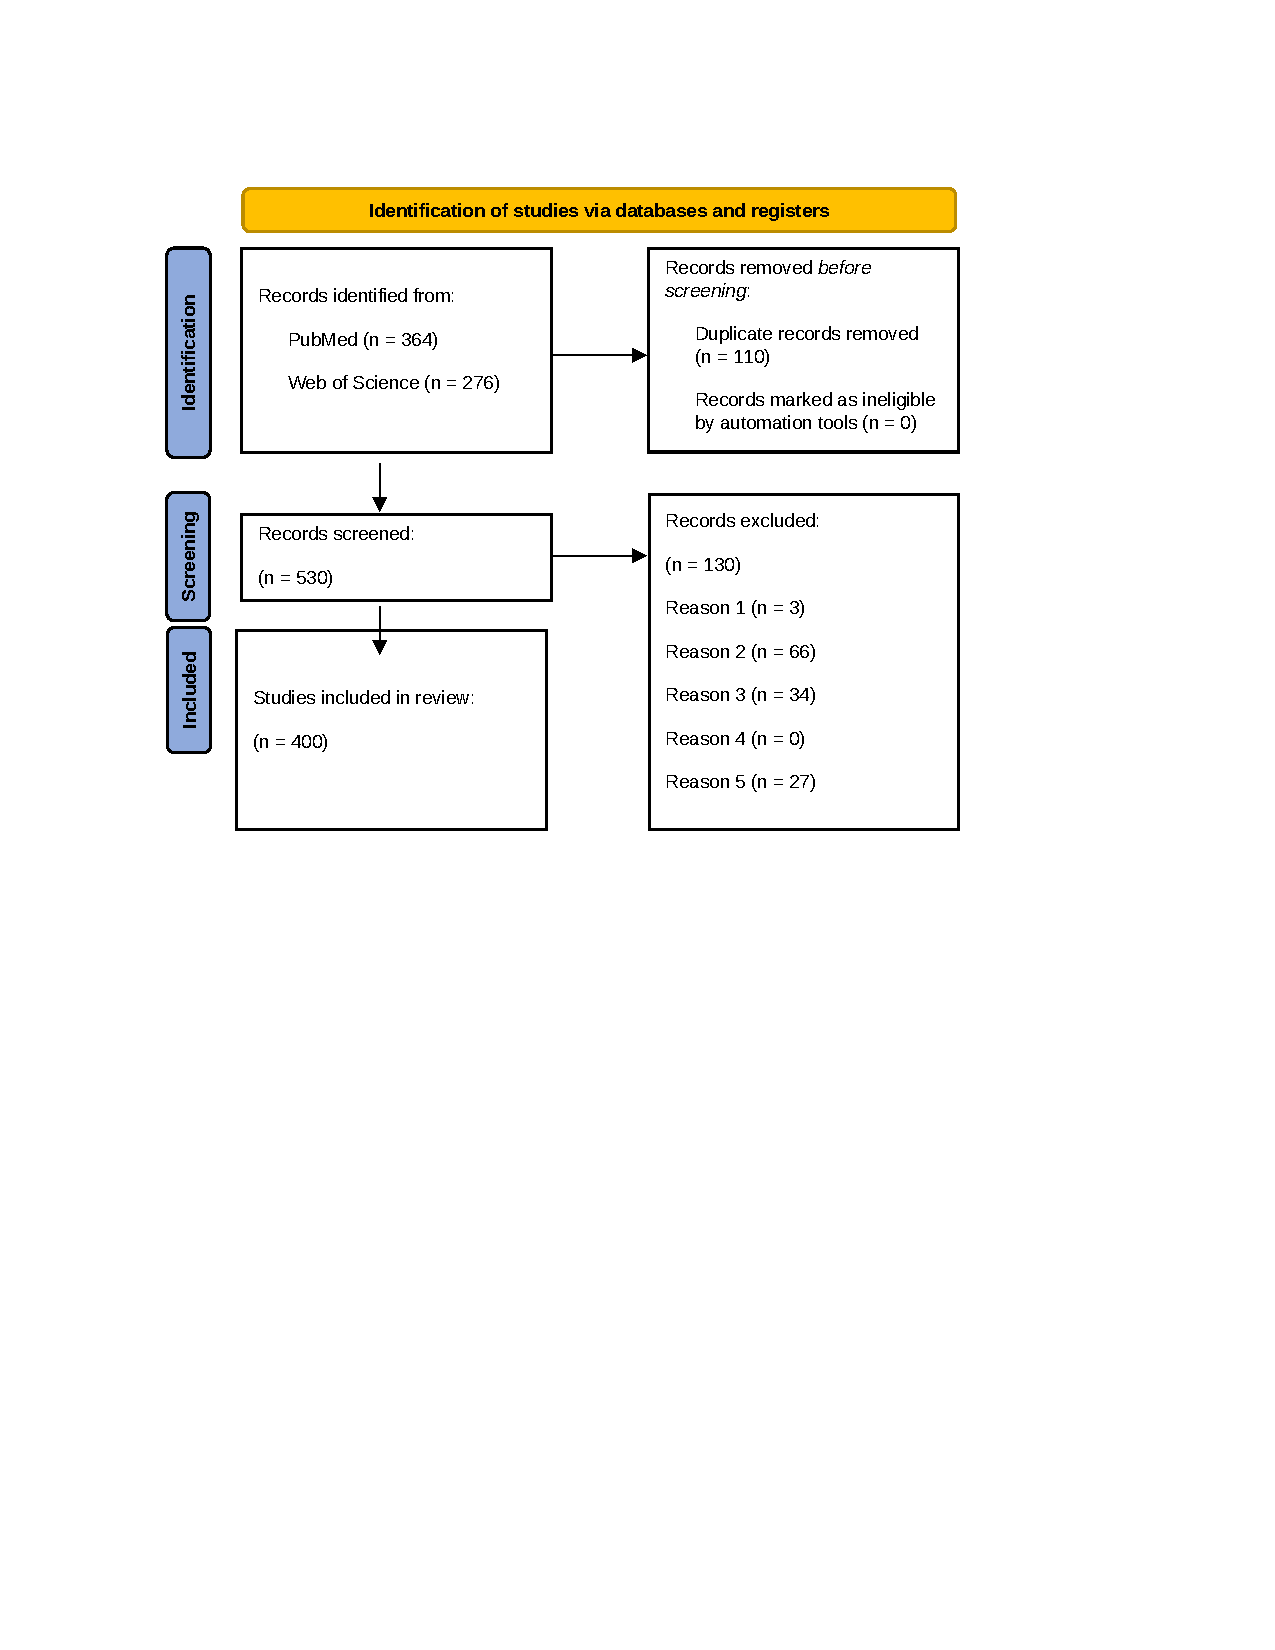
\includegraphics[scale=0.88]{images/flux.pdf}
	\caption[Diagramme de flux.]{Diagramme de flux. Les raisons 1 à 4 font référence aux critères du cadre PICO, la raison 5 à la langue et la raison 6 au type de document.}
	\label{fig:flux}
\end{figure}

\clearpage

\subsection*{Annexe B. Voie Akt/mTOR}\phantomsection \label{annexeB}

\begin{figure}[h]
	\centering
	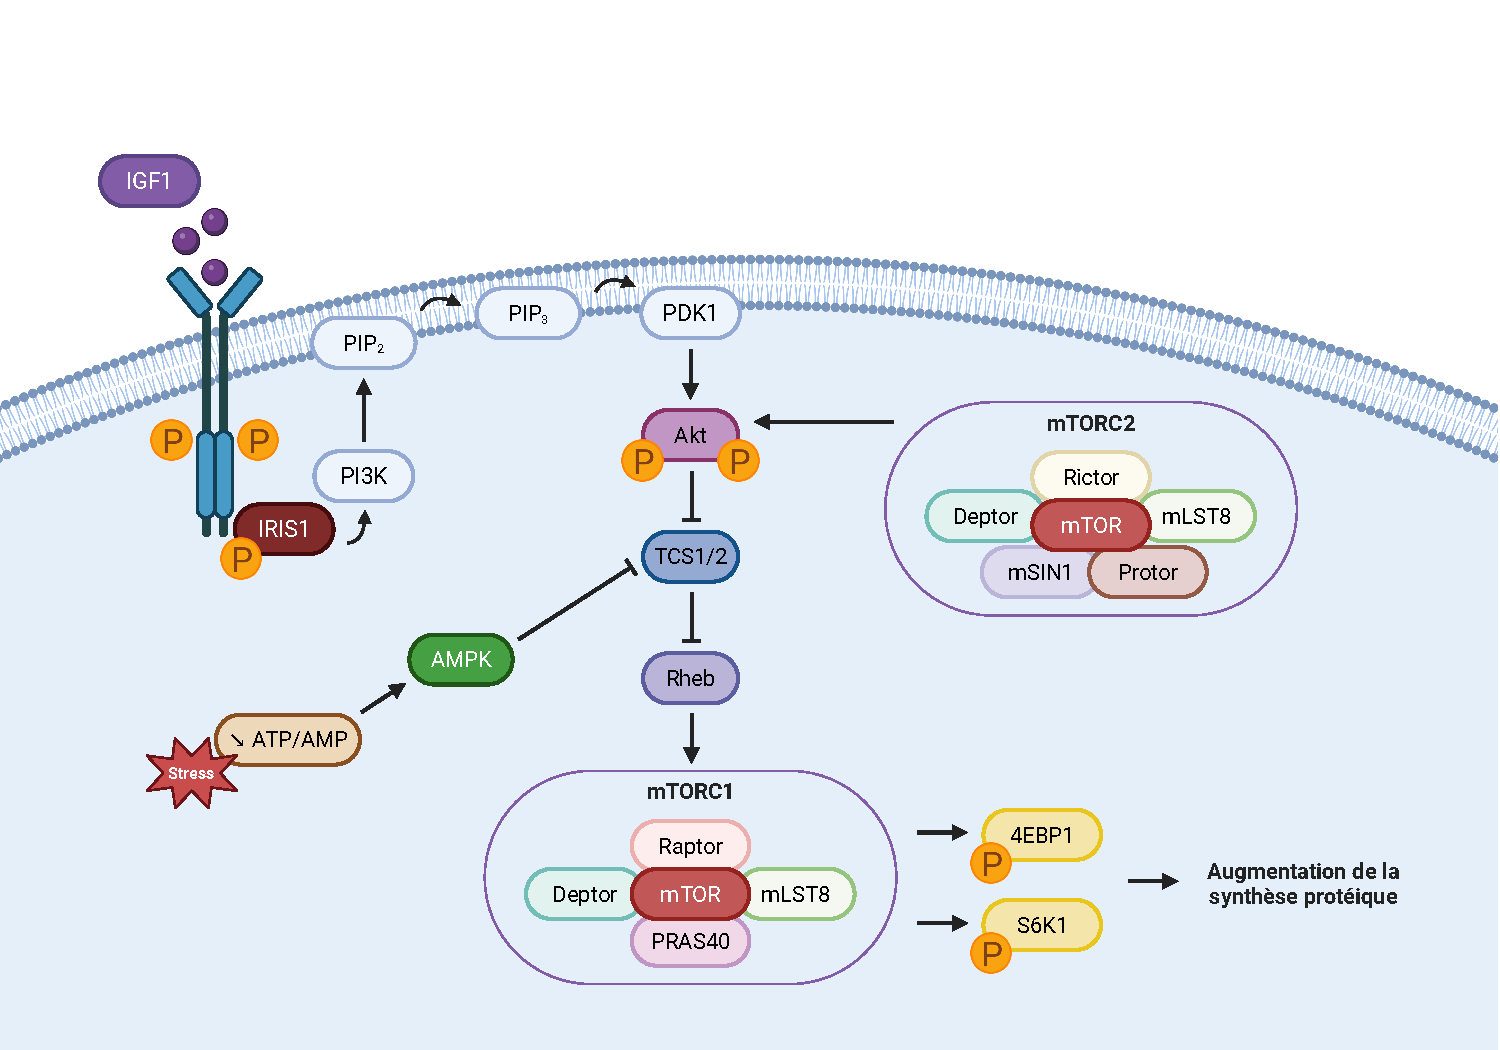
\includegraphics[scale=0.54]{images/Akt_mTOR.pdf}	
	\\ Créée avec \href{https://BioRender.com}{BioRender}, adaptée de 
	\parencite{Marafie2024Jun}.
\end{figure}

La voie Akt/mTOR est un régulateur majeur de la masse musculaire. Son activation stimule principalement la synthèse protéique \parencite{Egerman2013Nov}.

La voie est activée par la liaison d'IGF-1 à son récepteur membranaire IGF1R, une tyrosine kinase transmembranaire. Cette liaison induit la dimérisation et la trans-phosphorylation d'IGF1R sur des résidus tyrosine. Ces tyrosines phosphorylées constituent alors des sites d'ancrage pour la protéine adaptatrice IRS1, un substrat du récepteur à l'insuline 1, qui est ensuite elle-même phosphorylée. IRS1 phosphorylée recrute PI3K (phosphoinositide 3-kinase), une enzyme lipidique qui convertit le PIP2 (phosphatidylinositol diphosphate) en PIP3 (phosphatidylinositol triphosphate). L'accumulation de PIP3 permet le recrutement de PDK1 (3-phosphoinositide-dependent protein kinase-1) et d'Akt (protein kinase B) à la membrane. Akt est phosphorylé sur Thr308 par PDK1 et sur Ser473 par mTORC2, ce qui conduit à son activation complète.

Akt active le complexe mTORC1 en inhibant le complexe TSC1/2 (Tuberous Sclerosis Complex 1/2), permettant à Rheb (Ras homolog enriched in brain) d'activer mTORC1. À l'inverse, en conditions de stress énergétique, AMPK inhibe mTORC1 en renforçant l'action inhibitrice du complexe TSC1/2 \parencite{Marafie2024Jun}. Une fois activé, mTORC1 contrôle la synthèse protéique en phosphorylant la kinase S6K1 et 4EBP1. Ces protéines constituent les principales cibles en aval de la signalisation mTORC1 \parencite{Marafie2024Jun}. La phosphorylation de 4EBP1 permet l'initiation de la traduction dépendante de la coiffe des ARNm, tandis que la phosphorylation de S6K1 stimule la biogenèse des ARNm ainsi que l'initiation et l'élongation de la traduction \parencite{Laplante2012Apr}.

Ainsi, l'activation de la voie Akt/mTORC1 stimule la synthèse protéique favorisant la croissance cellulaire et l'augmentation de la masse musculaire. À l'inverse, l'inhibition de cette voie contribue à la diminution de la synthèse protéique observée lors de l'atrophie musculaire.

\newpage

\subsection*{Annexe C. Système des calpaines}\phantomsection \label{annexeC}

\begin{figure}[h]
	\centering
	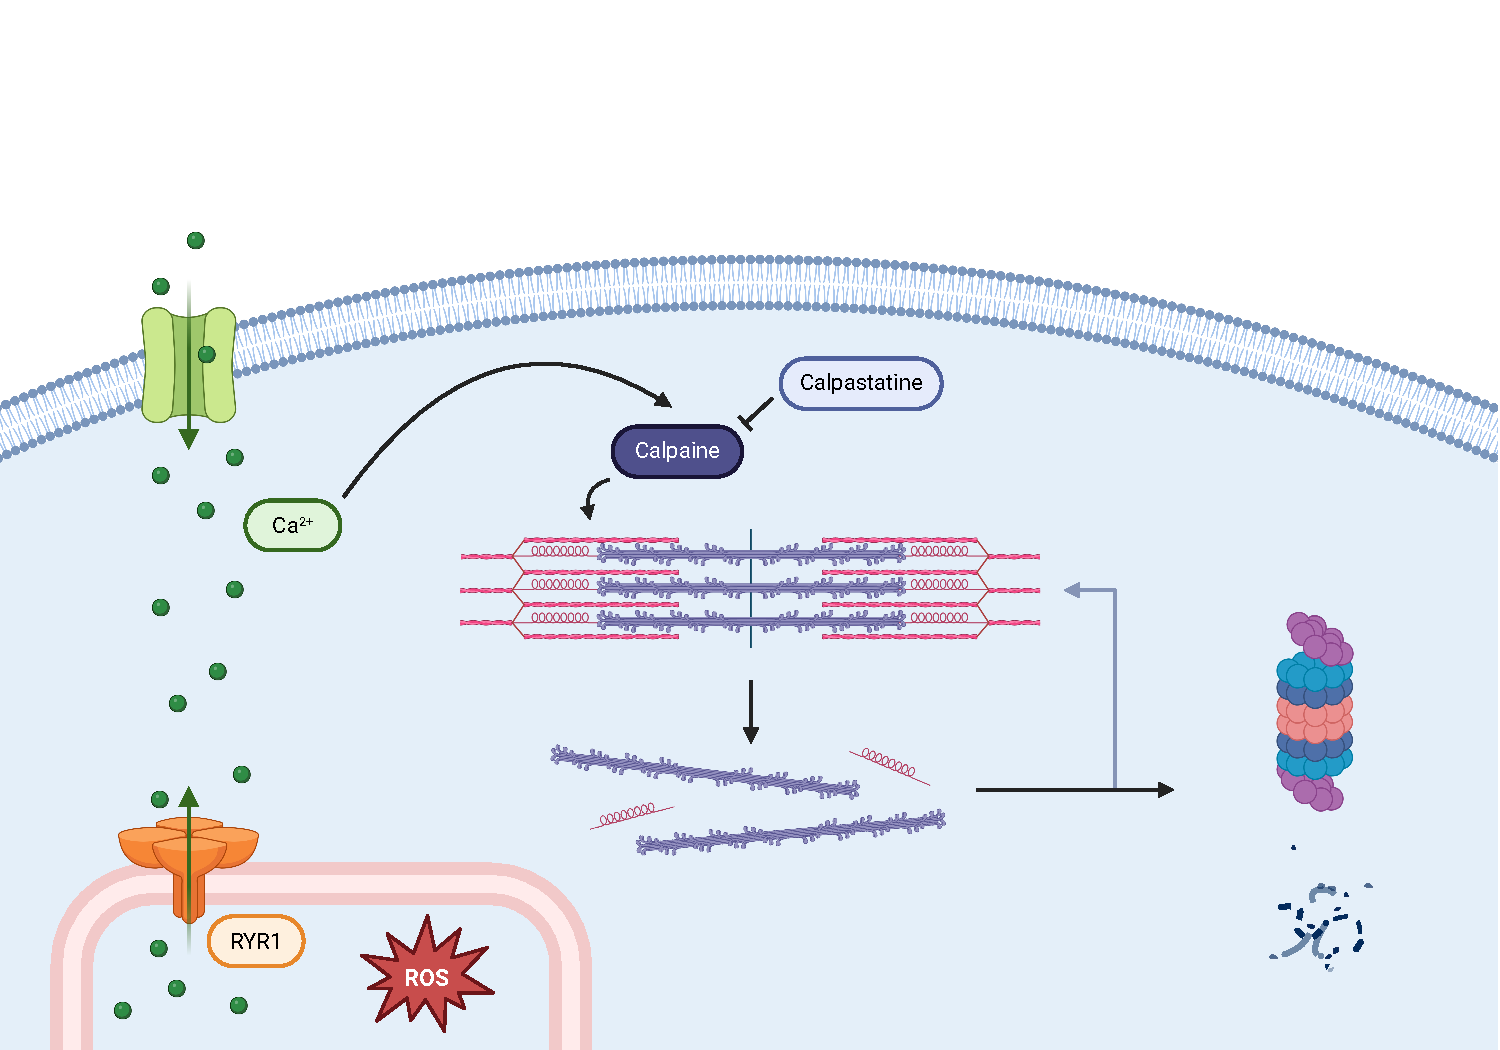
\includegraphics[scale=0.54]{images/Calpaine.pdf}	
	\\ Créée avec \href{https://BioRender.com}{BioRender}, adaptée de 
	\parencite{Huang2016Nov,Bartoli2005Oct}.
\end{figure}

Le système des calpaïnes constitue l'un des mécanismes initiateurs de la dégradation des myofibrilles dans le muscle \parencite{Bartoli2005Oct}. 

Les calpaïnes sont des protéases cystéine-dépendantes du Ca$^{2+}$ dont l'activité est étroitement contrôlée par leur inhibiteur endogène, la calpastatine. L'interaction entre les calpaïnes et la calpastatine est modulée par la concentration intracellulaire en Ca$^{2+}$ \parencite{Scicchitano2015}. À l'état basal, les calpaïnes sont présentes dans le cytosol sous une forme inactive. Une augmentation de la concentration intracellulaire en Ca$^{2+}$ induit un changement conformationnel permettant leur activation \parencite{Huang2016Nov}. Cette élévation du Ca$^{2+}$ peut résulter soit d'un influx de Ca$^{2+}$ extracellulaire via l'ouverture des canaux calciques, soit d'une fuite de Ca$^{2+}$ du réticulum sarcoplasmique. Cette fuite peut être favorisée par une augmentation de la production d'espèces réactives de l'oxygène (ROS), conduisant à l'oxydation du récepteur à la ryanodine (RYR1) \parencite{Hyatt2020Dec}.

Une fois activées, les calpaïnes entrainent la désorganisation du disque Z en clivant plusieurs protéines essentielles à l'intégrité structurale du sarcomère, notamment la nébuline, la titine et la filamine \parencite{Huang2016Nov}. Les filaments d'actine et de myosine, ainsi que d'autres protéines sarcomériques, sont alors passivement libérés dans le cytoplasme \parencite{Bartoli2005Oct}. Dans des conditions physiologiques, ces fragments myofibrillaires participent aux processus de remodelage cytosquelettique \parencite{Scicchitano2015}. En revanche, dans des conditions d'atrophie, ces fragments sont dirigés vers le système ubiquitine-protéasome où ils seront entièrement dégradés \parencite{Bartoli2005Oct}.

\newpage

\subsection*{Annexe D. Système ubiquitine-protéasome}\phantomsection \label{annexeD}

\begin{figure}[h]
	\centering
	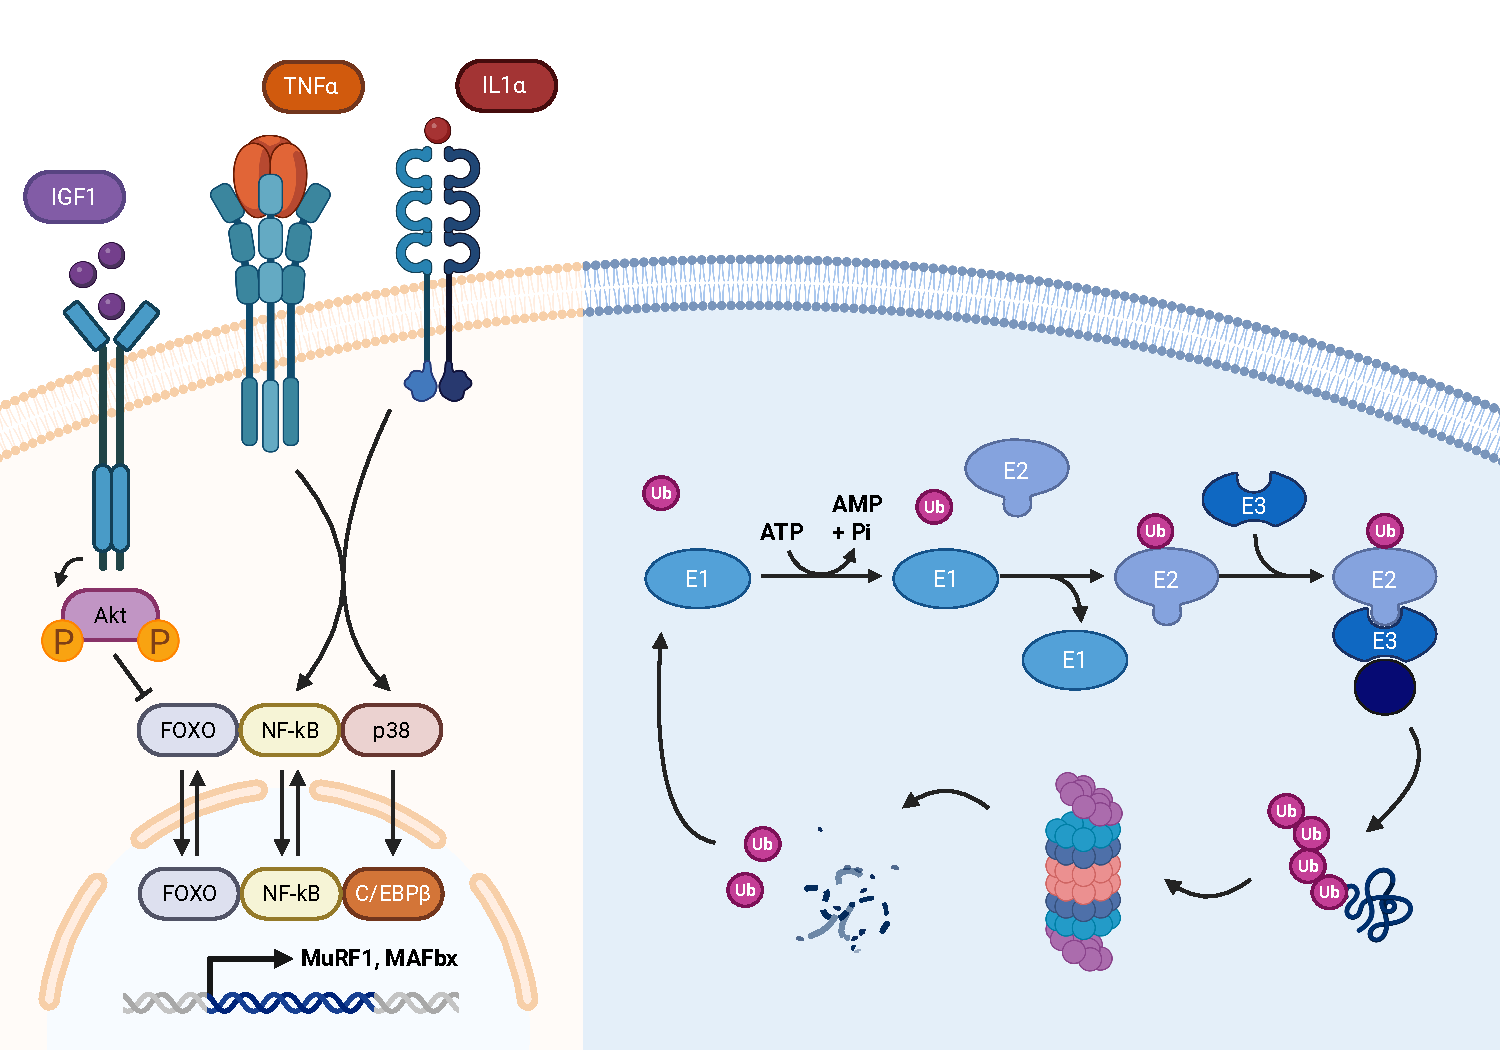
\includegraphics[scale=0.54]{images/Ubiquitine_protéasome.pdf}
	\\ Créée avec \href{https://BioRender.com}{BioRender}, adaptée de \parencite{Egerman2013Nov,Scicchitano2015}.
\end{figure}

Le système ubiquitine-protéasome constitue une voie majeure de dégradation protéique \parencite{Scicchitano2015}. Dans le muscle squelettique, son activation est associée à la perte de masse musculaire \parencite{Bodine2014Aug}. L'activation du système ubiquitine-protéasome repose sur l'augmentation de l'expression de MuRF1 et MAFbx, deux gènes codant pour des ubiquitine ligases E3 \parencite{Egerman2013Nov}. 

En conditions anaboliques, l'activation d'Akt inhibe la transcription de ces deux gènes en maintenant les facteurs de transcription FOXO dans le cytoplasme \parencite{Egerman2013Nov}. À l'inverse, en conditions d'atrophie, l'inactivation d'Akt entraîne la déphosphorylation des FOXO et leur translocation dans le noyau où ils induisent la transcription de MuRF1 et MAFbx \parencite{Scicchitano2015}. Par ailleurs, des cytokines pro-inflammatoires comme TNF-$\alpha$ et IL-1 peuvent activer les voies NF-$\kappa$B et MAP-K p38, participant aussi à l'augmentation de la transcription de MuRF1 et MAFbx \parencite{Egerman2013Nov}. L'augmentation de l'expression de ces ubiquitine ligases E3 dans le cytoplasme favorise l'ubiquitination de protéines spécifiques en vue de leur dégradation \parencite{Bodine2014Aug}. MuRF1 cible principalement les chaînes lourdes de myosine, tandis que MAFbx régule la synthèse protéique via notamment l'ubiquitination de eIF3c \parencite{Egerman2013Nov}.
 
Le processus d'ubiquitination implique une cascade enzymatique faisant intervenir les enzymes E1, E2 et E3. L'ubiquitine est d'abord activée de manière dépendante de l'ATP par une enzyme E1, formant une liaison thioester entre le groupement carboxy-terminal (COOH) de l'ubiquitine et la cystéine du site actif de l'E1. L'ubiquitine activée est ensuite transférée à une enzyme E2 à laquelle elle se lie également. Enfin, les ligases E3 catalysent la liaison covalente entre l'ubiquitine et un résidu lysine de la protéine cible \parencite{Bodine2014Aug}. Ces réactions se répètent pour former une chaîne polyubiquitine et les protéines ainsi marquées sont ensuite adressées, de manière dépendante de l'ATP, au protéasome 26S où elles sont dégradées. L'ubiquitine est finalement libérée et recyclée pour de nouveaux cycles enzymatiques \parencite{Scicchitano2015}.

\newpage

\subsection*{Annexe E. Voie autophagie-lysosome}\phantomsection \label{annexeE}

\begin{figure}[h]
	\centering
	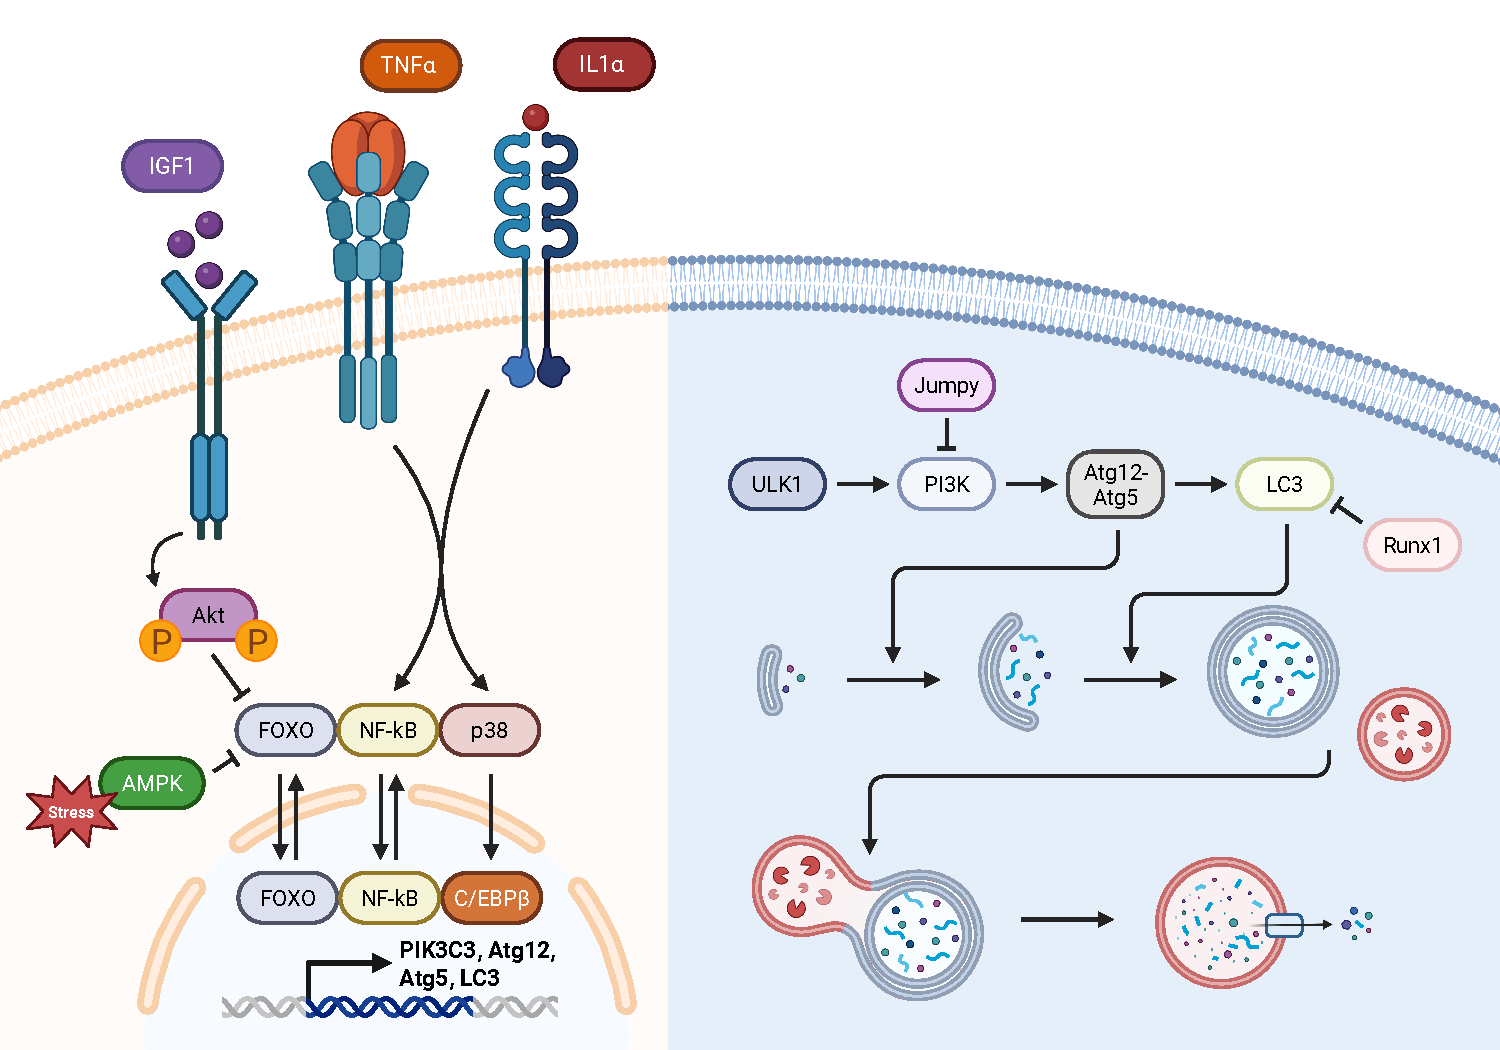
\includegraphics[scale=0.54]{images/Autophagie.pdf}
	\\ Créée avec \href{https://BioRender.com}{BioRender}, adaptée de \parencite{Ke2024Mar,Egerman2013Nov,Bechet2005Oct}.
\end{figure}

Le système autophagie-lysosome joue un rôle central dans le maintien de l'homéostasie cellulaire. À un niveau basal, l'autophagie permet le renouvellement des organites endommagés et la dégradation de protéines cytoplasmiques. En revanche, en conditions cataboliques, la suractivation de ce système contribue à l'atrophie musculaire \parencite{Scicchitano2015}. 

Le système autophagie-lysosome est principalement contrôlé par les facteurs de transcription FoxO. En effet, le stress oxydatif permet la translocation dans le noyau des FoxO qui induisent la transcription de gènes autophagiques tels que PIK3C3, Atg12, Atg5, LC3, Bnip3 et la cathepsine L. La voie p38 $\alpha\beta$ MAPK module également l'expression des gènes autophagiques en réponse au stress oxydatif. À l'inverse, en conditions anaboliques, Akt constitue l'inhibiteur principal de l'autophagie dans le muscle squelettique \parencite{Sandri2010Apr,Scicchitano2015}. Les gènes Runx1 et Jumpy peuvent aussi inhiber l'autophagie \parencite{Sandri2010Apr}.

L'autophagie implique la formation d'une vésicule cytosolique à double membrane, l'autophagosome, au cours de trois étapes successives \,---\,l'initiation, l'élongation et la maturation \,---\,\-\ qui permettent de séquestrer et transporter le matériel cytoplasmique vers le lysosome pour sa dégradation \parencite{Scicchitano2015,Bechet2005Oct}. Tout d'abord, le complexe ULK1 active la PI3K permettant la génération de la structure pré-autophagique qui délimite le cargo cytoplasmique. Puis, le complexe Atg12-Atg5 est nécessaire pour la croissance des membranes en forme de coupe et le recrutement de LC3, permettant la formation d'une vésicule complète \parencite{Bechet2005Oct}. BNIP3 favorise la mitophagie en conditions de stress, ciblant spécifiquement les mitochondries endommagées \parencite{Sandri2010Apr}. Une fois formé, l'autophagosome fusionne avec le lysosome pour former l'autolysosome. Les hydrolases lysosomales dégradent alors les protéines, organites et autres composants cytoplasmiques \parencite{Ke2024Mar}. La cathepsine L intervient à ce stade pour cliver le contenu autophagique et faciliter sa dégradation, permettant le recyclage des nutriments et la régénération énergétique \parencite{Sandri2010Apr}.

Ainsi, l'activation du système autophagie-lysosome assure le renouvellement cellulaire et, lorsqu'il est suractivé, contribue à la perte de masse musculaire observée lors de l'atrophie. 

\newpage

\subsection*{Annexe F. Critères d'inclusion et d'exclusion de l'étude AGBRESA}\phantomsection \label{annexeF}

\begin{table}[ht]
	\centering
	\renewcommand{\arraystretch}{1.7}
	\begin{tabularx}{\textwidth}{
			>{\raggedright\arraybackslash}X  % Critères d'inclusion
			>{\raggedright\arraybackslash}X  % Critères d'exclusion
		}
		\hline
		\textbf{Critères d'inclusion} & \textbf{Critères d'exclusion} \\
		\hline
		Être en bonne santé physique et psychologique 
		& Suivre un régime strictement végétarien ou végétalien \\
		
		Avoir un âge compris entre 24 et 55 ans 
		& Présenter des conduites addictives \\
		
		Avoir une taille comprise entre 153 et 190 cm 
		& Présenter une pathologie susceptible de contre-indiquer la participation à l'étude \\
		
		Avoir un IMC compris entre 19 et 30 kg.m$^{-2}$ 
		& Présenter un implant métallique incompatible avec l'IRM \\
		
		Être non-fumeur ou avoir cessé le tabac depuis au moins 6 mois 
		& Prendre un traitement médicamenteux soumis à prescription, y compris les contraceptifs hormonaux \\
		
		Posséder une assurance maladie 
		& Avoir, pour les femmes, un cycle menstruel irrégulier (hors 26–32 jours) \\
		
		Présenter un casier judiciaire vierge 
		&  \\
		\hline
	\end{tabularx}
\end{table}

Pour plus de détails, voir \textcite{Clement2022Sep}.

\newpage

\subsection*{Annexe G. Protéines d'intérêt et anticorps primaires utilisés}\phantomsection \label{annexeG}

\begin{table}[ht]
	\centering
	\renewcommand{\arraystretch}{1.7}
	\begin{tabularx}{\textwidth}{
			>{\raggedright\arraybackslash}X
			>{\centering\arraybackslash}p{1.7cm}
			>{\centering\arraybackslash}X
			>{\centering\arraybackslash}p{1.7cm}
			>{\centering\arraybackslash}p{3cm}
			>{\centering\arraybackslash}X
			>{\centering\arraybackslash}X
		}
		\hline
		\textbf{Cible} &
		\textbf{Poids (kDa)} &
		\textbf{Dilution} &
		\textbf{Hôte} &
		\textbf{Fabriquant} &
		\textbf{Référence} &
		\textbf{Classe} \\
		\hline
		Myosine & 200 & 1:1000 & mouse & Santa cruz & 376157 & monoclonal \\
		Ubiquitine & / & 1:1000 & rabbit & Cell signaling & 3933 & polyclonal \\
		P-p38 & 40 & 1:1000 & rabbit & Cell signaling & 9211 & polyclonal \\
		P-AMPK & 62 & 1:1000 & rabbit & Cell signaling & 2535 & monoclonal \\
		MuRF1 & 40 & 1:2000 & rabbit & Abcam & 172479 & monoclonal \\
		P-Akt & 60 & 1:1000 & rabbit & Cell signaling & 9271 & polyclonal \\
		P-4EBP1 & 15-20 & 1:1000 & rabbit & Cell signaling & 2855 & monoclonal \\
		P-p70S6K & 70 & 1:1000 & rabbit & Cell signaling & 9234 & monoclonal \\
		PGC1-$\alpha$ & 75 & 1:1000 & rabbit & Cell signaling & 2178 & monoclonal \\
		Cox IV & 17 & 1:1000 & rabbit & Cell signaling & 4844 & polyclonal \\
		Cyt c & 15 & 1:1000 & mouse & Santa cruz & 13156 & monoclonal \\
		\hline
	\end{tabularx}
\end{table}

Le préfixe "P-" indique la forme phosphorylée de la protéine, correspondant à son état activé.

\newpage

\subsection*{Annexe H. Caractéristiques cliniques et paramètres systémiques des participants}\phantomsection \label{annexeH}

Les valeurs moyennes ($\pm$ écart-type) des caractéristiques cliniques des 5 participants étaient, en condition BDC-4, de 76,24 $\pm$ 13,31 kg pour la masse corporelle totale, avec 70,5 $\pm$ 4,9\% de masse maigre et 25,4 $\pm$ 4,6\% de masse grasse. En condition HDT60, ces valeurs étaient respectivement de 74,09 $\pm$ 13,18\%, 67,7 $\pm$ 4,3\% et 28,1 $\pm$ 4,0\%. La cinétique sur toute la durée du protocole de ces caractéristiques cliniques est présentée en \hyperref[annexeH]{annexe I}.

\begin{table}[ht]
	\centering
	\renewcommand{\arraystretch}{1.7}
	\begin{tabularx}{\textwidth}{
			>{\raggedright\arraybackslash}X
			>{\centering\arraybackslash}X
			>{\centering\arraybackslash}X
			>{\centering\arraybackslash}X
			>{\centering\arraybackslash}X
			>{\centering\arraybackslash}X
			>{\centering\arraybackslash}X
		}
		\hline
		\textbf{Sujet} &
		\textbf{Masse totale BDC-4 (kg)} &
		\textbf{Masse totale HDT60 (kg)} &
		\textbf{Masse grasse BDC-4 (\%)} &
		\textbf{Masse grasse HDT60 (\%)} &
		\textbf{Masse maigre BDC-4 (\%)} &
		\textbf{Masse maigre HDT60 (\%)} \\
		\hline
		D & 80,53 & 77,19 & 31,7 & 33,4 & 63,9 & 62,1 \\
		F & 76,40 & 74,63 & 20,1 & 22,8 & 76,0 & 73,2 \\
		J & 81,33 & 80,41 & 23,0 & 26,6 & 73,7 & 70,1 \\
		T & 53,87 & 51,85 & 23,8 & 27,2 & 71,6 & 67,9 \\
		W & 89,06 & 86,36 & 28,2 & 30,3 & 67,4 & 65,2 \\
		\hline
	\end{tabularx}
\end{table}

F, J, W, D et D désignent les sujets. BDC-4 correspond au quatrième jour précédant le début du protocole d'alitement à -6°, et HDT60 correspond au soixantième jour de ce protocole.

\vspace*{2.5em}

Les valeurs moyennes ($\pm$ écart-type) des paramètres systémiques des participants s'élevaient, en condition BDC-6, à 58,2 $\pm$ 48,9 $\mu$g.L$^{-1}$ pour la ferritine, 0,87 $\pm$ 0,99 mg.L$^{-1}$ pour la CRP et 1,04 $\pm$ 0,58 g.L$^{-1}$ pour l'haptoglobine. En condition HDT6, ces valeurs étaient respectivement de 62,0 $\pm$ 51,7 $\mu$g.L$^{-1}$, 0,43 $\pm$ 0,37 mg.L$^{-1}$ et 1,05 $\pm$ 0,44 g.L$^{-1}$.

\begin{table}[ht]
	\centering
	\renewcommand{\arraystretch}{1.7}
	\begin{tabularx}{\textwidth}{
			>{\raggedright\arraybackslash}p{1.2cm}   % Sujet (réduit)
			>{\centering\arraybackslash}p{2.2cm}    % Ferritine BDC-6
			>{\centering\arraybackslash}p{2.2cm}    % Ferritine HDT6
			>{\centering\arraybackslash}p{1.8cm}    % CRP BDC-6
			>{\centering\arraybackslash}p{1.8cm}    % CRP HDT6
			>{\centering\arraybackslash}X           % Haptoglobine BDC-6 (large)
			>{\centering\arraybackslash}X           % Haptoglobine HDT6 (large)
		}
		\hline
		\textbf{Sujet} &
		\textbf{Ferritine BDC-6 ($\mu$g.L$^{-1}$)} &
		\textbf{Ferritine HDT6 ($\mu$g.L$^{-1}$)} &
		\textbf{CRP BDC-6 (mg.L$^{-1}$)} &
		\textbf{CRP HDT6 (mg.L$^{-1}$)} &
		\textbf{Haptoglobine BDC-6 (g.L$^{-1}$)} &
		\textbf{Haptoglobine HDT6 (g.L$^{-1}$)} \\
		\hline
		D & 31 & 35 & 0,41 & 0,00 & 0,80 & 0,90 \\
		F & 142 & 151 & 0,00 & 0,20 & 1,27 & 1,22 \\
		J & 38 & 30 & 2,45 & 0,65 & 0,76 & 0,79 \\
		T & 21 & 30 & 0,29 & 0,35 & 0,43 & 0,61 \\
		W & 59 & 64 & 1,20 & 0,93 & 1,93 & 1,74 \\
		\hline
	\end{tabularx}
\end{table}

F, J, W, D et D désignent les sujets. BDC-6 correspond au sixième jour précédant le début du protocole d'alitement à -6°, et HDT60 correspond au soixantième jour de ce protocole.

\subsection*{Annexe I. Cinétique des caractéristiques cliniques des sujets au cours du protocole}\phantomsection \label{annexeI}
\begin{center}
	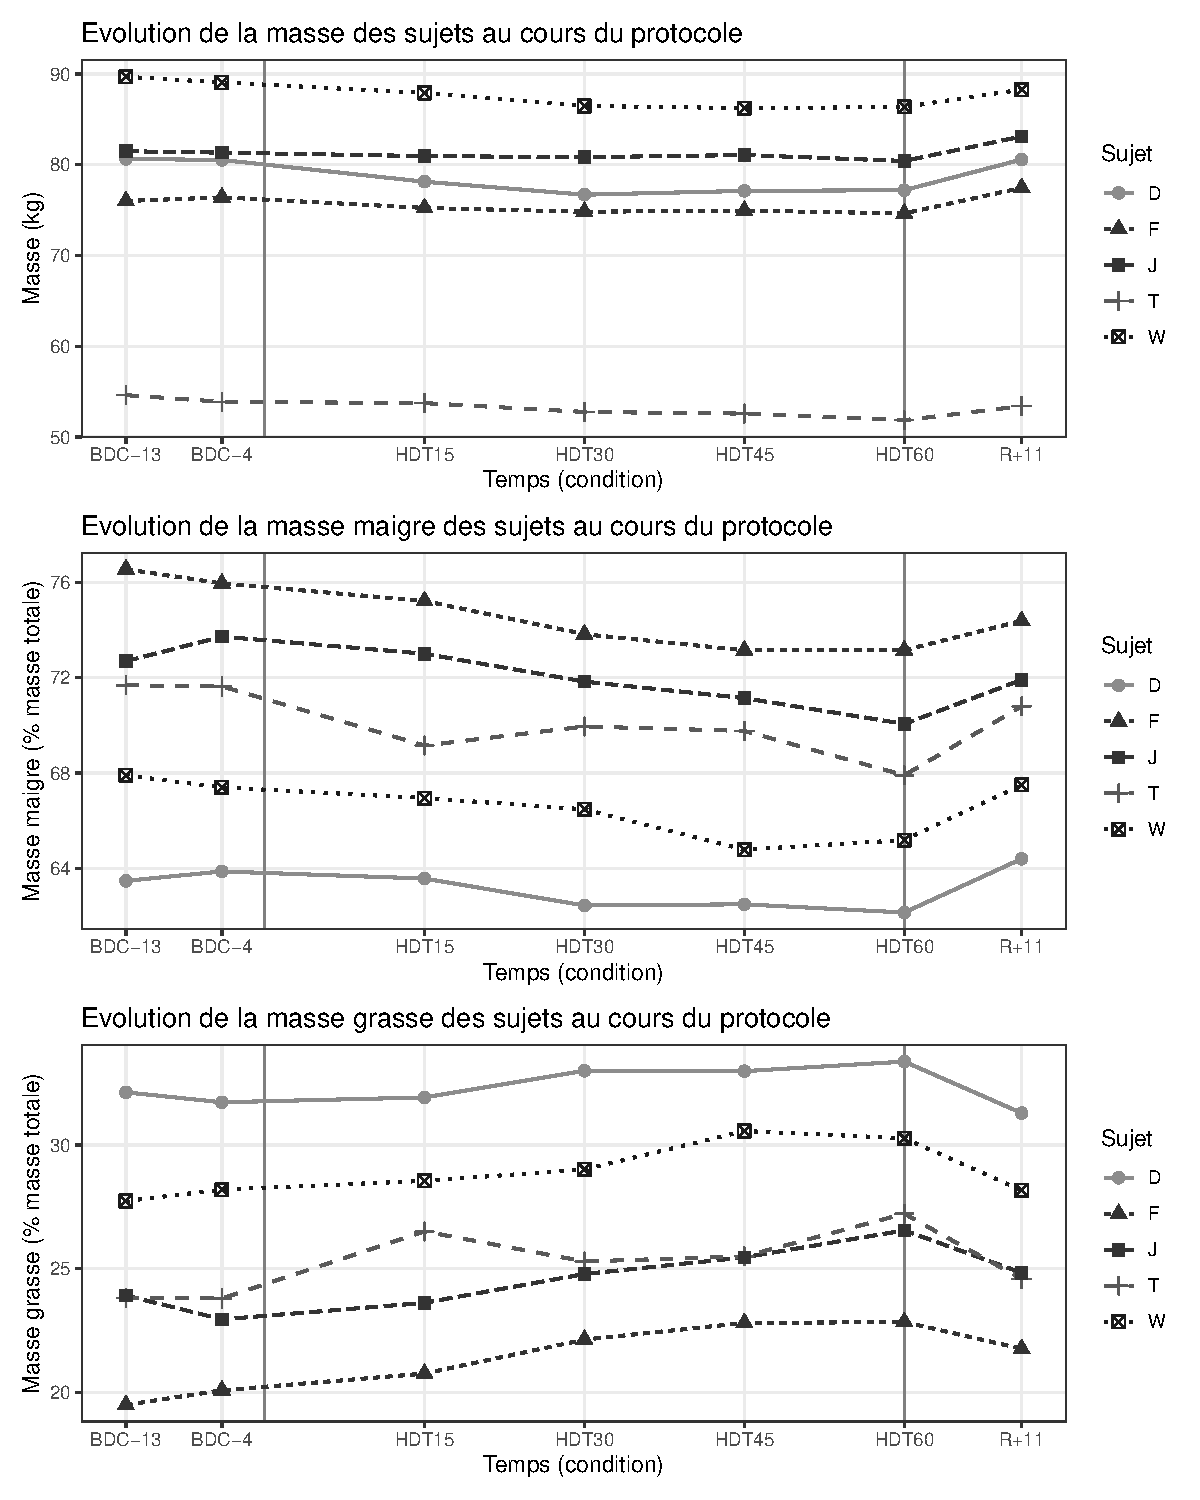
\includegraphics[width=\textwidth]{images/masse_totale_maigre_grasse.pdf}	
\end{center}
F, J, W, D et D désignent les sujets. BDC-X correspond au Xième jour précédant le début du protocole d'alitement à -6°, HDTX correspond au Xième jour de ce protocole, et R+X au Xième jour de la phase de récupération. Les lignes verticales représentent le début et la fin de la phase d'alitement.

\newpage

\subsection*{Annexe J. Résultats des Western Blot}\phantomsection \label{annexeJ}

\begin{center}
	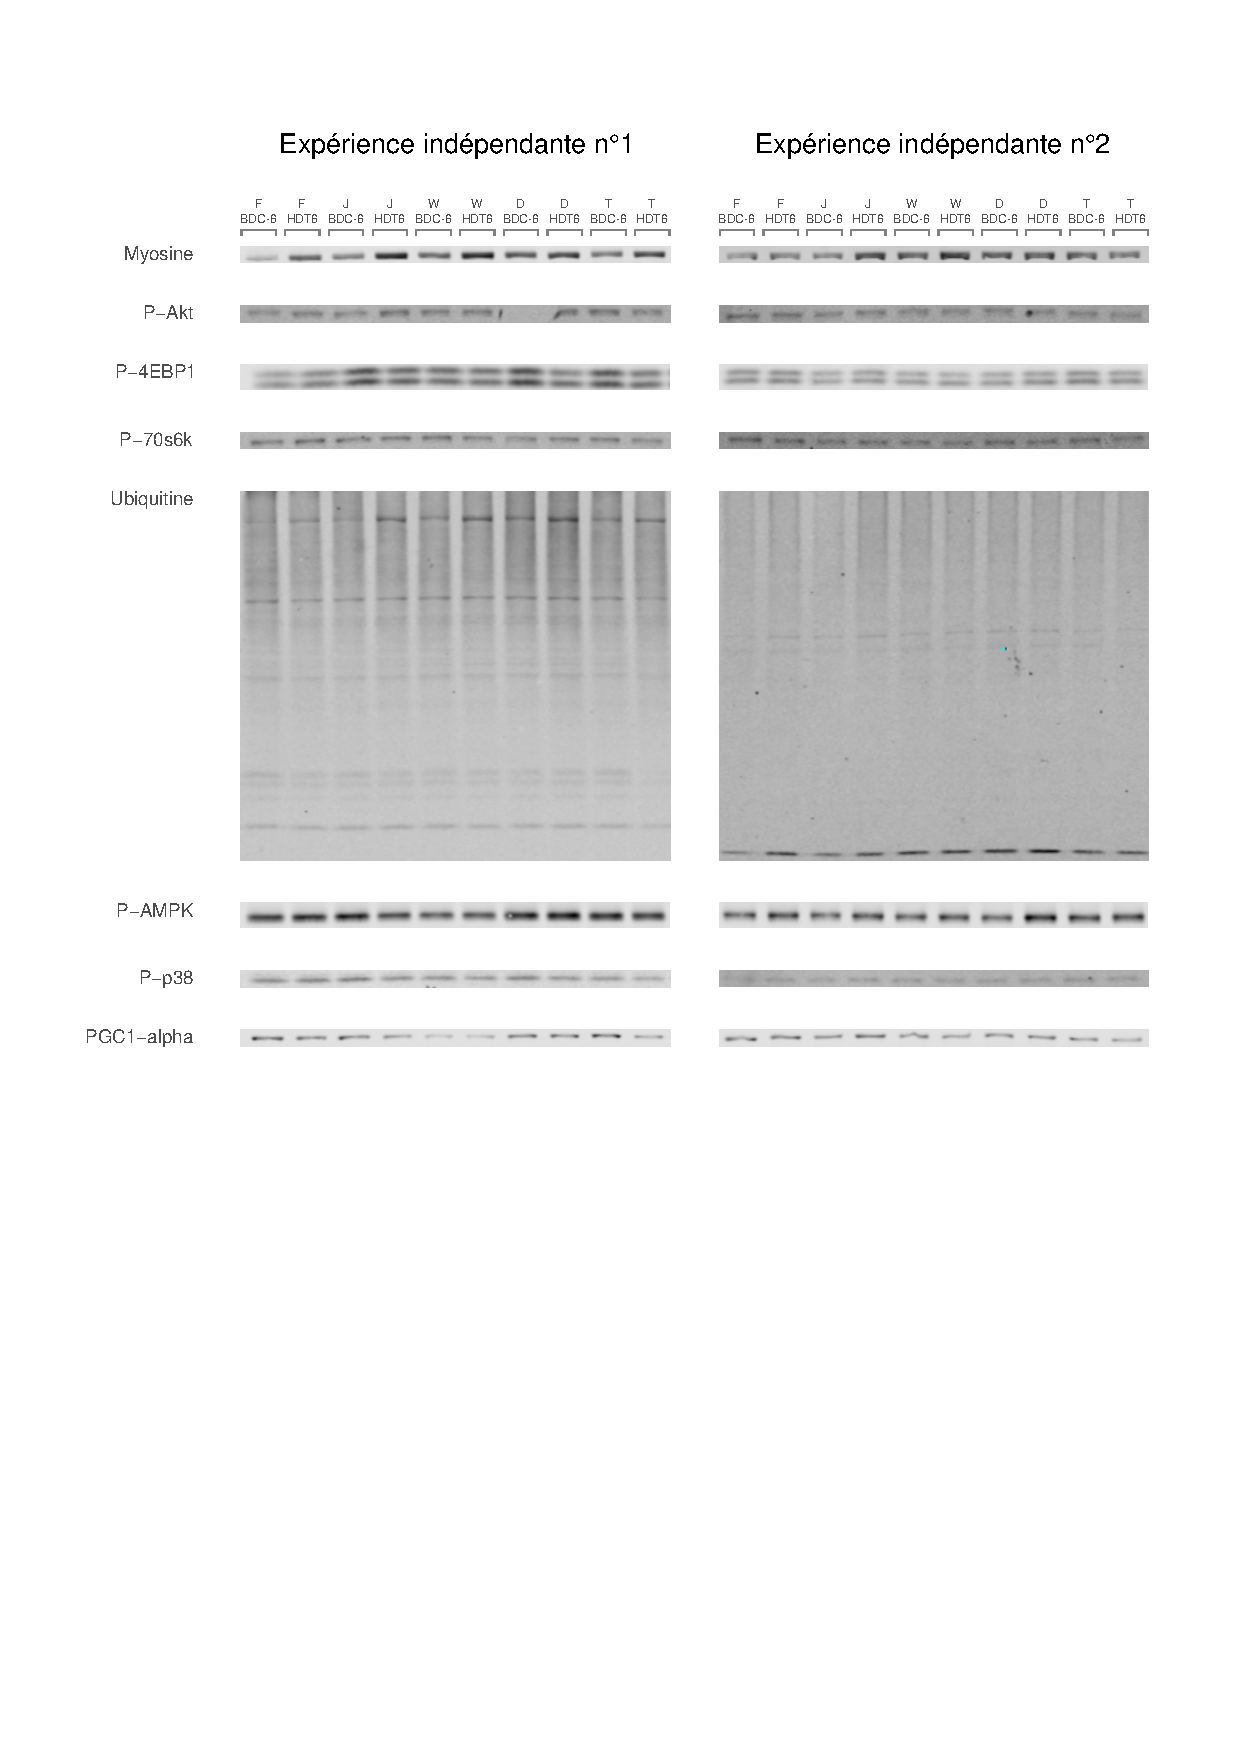
\includegraphics[width=\textwidth]{images/annexe résultats WB.pdf}	
\end{center}
F, J, W, D et D désignent les sujets. BDC-6 correspond au sixième jour précédant le début du protocole d'alitement à -6°, et HDT6 correspond au sixième jour de ce protocole.

\newpage

\normalsize 

\newgeometry{hmargin=1.5cm, vmargin=1.5cm}
\begin{wrapfigure}[3]{r}{2.5cm}
\vspace{-6mm}

\includegraphics[width =2.5cm]{images/ens.pdf}
\end{wrapfigure}

\noindent\normalsize{Ecole normale supérieure de Rennes}
\vspace{0.01\baselineskip}

\noindent\normalsize{Département Sciences du sport et éducation physique}
\vspace{0.01\baselineskip}

\noindent\normalsize{Année 2025-2026 -- Diplôme de l'ENS -- 2\textsuperscript{e} année}

\hrulefill

\begin{center}
  {\bf{\Large{Effet de l'environnement systémique de volontaires exposés à la microgravité simulée sur le phénotype contractile et métabolique de myotubes murins}}}
\end{center}
\vspace{0.01\baselineskip}
{\bf{\textit{Présenté par : Léonine ROUANET}}}

\textit{Sous la direction de : Frédéric Derbré (Université Rennes 2)}
\singlespacing
\small{{\bf{RÉSUMÉ}}}

 \footnotesize{{\bf{Objectif}} : Ce mémoire visait à déterminer si l'environnement systémique avait un effet sur le muscle squelettique d'individus exposés à la microgravité simulée. Nous avons fait l'hypothèse que l'environnement systémique induirait un phénotype d'atrophie musculaire.
 	
 {\bf{Méthode}} : Des myotubes C2C12 ont été exposés pendant 48 heures à du plasma prélevé 6 jours avant (BDC-6) et 6 jours après un protocole d'alitement à -6° (HDT6). Le diamètre des myotubes et l'expression des chaînes lourdes de myosine, ainsi que de protéines impliquées dans la synthèse protéique (p-Akt, p-4EBP1, p-p70S6K), la dégradation protéique (protéines ubiquitinées), le stress cellulaire (p-p38, p-AMPK) et la biogenèse mitochondriale (PGC1-$\alpha$) ont été analysés.
 
 {\bf{Résultats}} : Le diamètre moyen des myotubes est resté inchangé entre les conditions BDC-6 et HDT6, sans signe d'atrophie macroscopique ($\beta$ = 0,30 $\mu$m, IC$_{95\%}$ = [-0,61 ; 1,13]). Le plasma post-alitement n'a pas non plus induit les voies de signalisation classiquement associées à l'atrophie musculaire. Cependant, une augmentation de l'expression des chaînes lourdes de myosine a été observée en condition HDT6, bien que cet effet demeure incertain ($\beta$ = 1,56 ratio HDT6/BDC-6, IC$_{95\%}$ = [1,16 ; 1,98]).
 
 {\bf{Discussion}} : Une inflammation de bas grade ne peut être totalement exclue chez nos participants, mais elle reste vraisemblablement limitée, ce qui contribue certainement à expliquer l'absence d'effet de la condition HDT6 sur le diamètre des myotubes et sur l'expression des protéines d'intérêt, à l'exception des chaînes lourdes de myosine. Cette augmentation de l'expression des chaînes lourdes de myosine en condition HDT6 paraît peu cohérente avec l'absence d'effet observée par ailleurs.
 
 {\bf{Conclusion}} : En dépit de cette observation, nos résultats renforcent l'idée que l'absence de contraintes mécaniques constitue le déterminant principal de l'atrophie observée en microgravité. Ils soutiennent ainsi l'intérêt des exercices physiques dans la prévention du déconditionnement musculaire, tant chez les astronautes que chez les patients alités sur Terre.}

\medskip

{\bf{Mots-clefs : atrophie, myotubes, milieu conditionné, inflammation, microgravité simulée.}}

\vspace{1\baselineskip}

\small{{\bf{ABSTRACT}}}

 \footnotesize{{\bf{Objective}}: This work aimed to determine whether the systemic environment affects skeletal muscle in individuals exposed to simulated microgravity. We hypothesized that the systemic environment would induce a muscle atrophy phenotype. 
 
 {\bf{Methods}}: C2C12 myotubes were exposed for 48 hours to plasma collected 6 days before (BDC-6) and 6 days after a head-down tilt bed rest protocol (HDT6). Myotube diameter and expression of myosin heavy chain isoforms were analysed, together with proteins involved in protein synthesis (p-Akt, p-4EBP1, p-p70S6K), protein degradation (ubiquitinated proteins), cellular stress (p-p38, p-AMPK), and mitochondrial biogenesis (PGC-1$\alpha$).
 
 {\bf{Results}}: Mean myotube diameter remained unchanged between BDC-6 and HDT6 conditions, with no evidence of macroscopic atrophy ($\beta$ = 0,30 $\mu$m, IC$_{95\%}$ = [-0,61 ; 1,13]). Plasma collected after bed rest did not induce signaling pathways commonly associated with muscle atrophy. However, an increase in myosin heavy chain expression was observed under the HDT6 condition, although this effect remains uncertain ($\beta$ = 1,56 HDT6/BDC-6 ratio, IC$_{95\%}$ = [1,16 ; 1,98]).
 
 {\bf{Discussion}}: Low-grade inflammation cannot be fully excluded in our participants, but it is likely to have been limited, which may explain the absence of an effect of the HDT6 condition on myotube diameter and on the expression of the proteins of interest, with the exception of myosin heavy chains. This increase in myosin heavy chain expression under HDT6 appears difficult to reconcile with the otherwise absent effects.
 
 {\bf{Conclusion}}: Despite this observation, our results reinforce the idea that mechanical unloading is the primary determinant of atrophy observed in microgravity. They further support the importance of physical exercise in preventing muscle deconditioning, both in astronauts and in bedridden patients on Earth.}

\medskip
	
{\bf{Keywords: atrophy, myotubes, conditioned media, inflammation, simulated microgravity.}}

\vspace{1\baselineskip}

{leonine.rouanet@ens-rennes.fr}


\end{document}
